\documentclass[12pt]{cmuthesis}
%\usepackage{fullpage,cmu-titlepage2}
\usepackage{times}
\usepackage[letterpaper,twoside,vscale=.8,hscale=.75,nomarginpar,hmarginratio=1:1]{geometry}
\usepackage{xcolor,colortbl}

\usepackage[
%backref controls whether the bibliography has a list of backreferences
%to where the citaiton is used
%backref,
pageanchor=true,
plainpages=false,
pdfpagelabels, % makes the status line page labels the same as latex ones
bookmarks,
bookmarksnumbered,
pdfborder=0 0 0,
pdfpagemode=UseOutlines]{hyperref}

\usepackage{apacite}
\usepackage{amsthm}
\usepackage{amsmath}
\usepackage{amssymb}

% For underbracket
\usepackage{mathtools}

\usepackage[bbsets,Dfprime]{math}
\usepackage[prefixflatinterpret,bracketmodalinterpret,modernsign,substopindex,shortmquant,mquantifiertype,mconnectiveformal,bracketinterpret,fixformat,setfixinterpret,modifopindex,seqarrow,seqoptional,sidenotecalculus,abbrseqcontext,shortterms,nosigmaterms,novarterms]{logic}
\usepackage[pretest,nocommandblocks]{progreg}
\usepackage[bracketinterpret,prefixflatinterpret,bracketmodalinterpret,fixformat,differentialdL]{dL}

\usepackage{booktabs}
\usepackage{tabularx}
\usepackage{subcaption}
\usepackage{verbatim}
\usepackage{framed}
\usepackage{tikz}
\usetikzlibrary{shapes,snakes}
\usepackage{pgfplots}
\usepackage{alltt}
\usetikzlibrary{arrows}
\usetikzlibrary{calc}
\usetikzlibrary{fit}
\usetikzlibrary{positioning,shadows}
\usetikzlibrary{automata}
\usetikzlibrary{shapes,arrows}
\usetikzlibrary{decorations.text}
\usetikzlibrary{decorations.markings}
\usetikzlibrary{trees,snakes}
\usepackage{graphicx}
\usepackage{paralist}
\usepackage{bussproofs}
\usepackage{proof}
\usepackage{lscape}
\usepackage{accents}


\newtheorem{theorem}{Theorem}
\newtheorem{proposition}[theorem]{Proposition}
\newtheorem{lemma}[theorem]{Lemma}
\newtheorem{corollary}[theorem]{Corollary}
\theoremstyle{definition}
\newtheorem{definition}{Definition}
\theoremstyle{remark}
\newtheorem{remark}{Remark}
\newtheorem{example}{Example}
\newcommand{\stepsto}{\mapsto}
\newcommand{\bebecomes}{\mathrel{::=}}
\newcommand{\alternative}{~|~}
\newcommand{\ivr}{\psi}
\newcommand{\meps}[2]{\iota{#1}~{#2}}
\newcommand{\xgivar}{\textsf{xi}}
\newcommand{\ygivar}{\textsf{yi}}
\newcommand{\xgvar}{\textsf{x}}
\newcommand{\ygvar}{\textsf{y}}
\newcommand{\xcvar}{\textsf{xc}}
\newcommand{\ycvar}{\textsf{yc}}
\newcommand{\ytvar}{\textsf{yt}}
%\newcommand{\xivar}{\textsf{xi}}
%\newcommand{\yivar}{\textsf{yi}}
%\newcommand{\xvar}{\textsf{x}}
\newcommand{\yvar}{\textsf{y}}
\newcommand{\wvar}{\textsf{w}}
\newcommand{\dxvar}{\textsf{dx}}
\newcommand{\dyvar}{\textsf{dy}}
\newcommand{\dxivar}{\textsf{dxi}}
\newcommand{\dyivar}{\textsf{dyi}}
\newcommand{\dxgvar}{\textsf{dxg}}
\newcommand{\dygvar}{\textsf{dyg}}
\newcommand{\kvar}{\textsf{k}}
\newcommand{\tvar}{\textsf{t}}
\newcommand{\vivar}{\textsf{vi}}
\newcommand{\vlvar}{\textsf{vl}}
\newcommand{\vhvar}{\textsf{vh}}
\newcommand{\obsvar}{{\sf obs}\xspace}
\newcommand{\Tvar}{{\sf T}\xspace}
\newcommand{\Avar}{{\sf A}\xspace}
\newcommand{\Bvar}{{\sf B}\xspace}
%\newcommand{\SBvar}{{\it SB }\xspace}
\newcommand{\xvar}{{\sf x}\xspace}
\newcommand{\vvar}{{\sf v}\xspace}
\newcommand{\avar}{{\sf a}\xspace}
\newcommand{\ctrl}{\textsf{ctrl}\xspace}
\newcommand{\ctrlliv}{\ctrl_{\text{a}}}
\newcommand{\plant}{\textsf{plant}\xspace}
\newcommand{\psimp}{\ensuremath{\alpha_{SV}}\xspace}
\newcommand{\sandbox}{\textsf{\upshape sandbox}\xspace}
\newcommand{\fallback}{\textsf{\upshape fallback}\xspace}
\newcommand{\verifiedmodelbody}{\ensuremath{\ctrl;\plant}}
\newcommand{\verifiedmodel}{\ensuremath{\prepeat{(\verifiedmodelbody)}}}
\newcommand{\exctrl}{\textsf{ctrl}_{SV}\xspace}
\newcommand{\pdrive}{\textsf{go}\xspace}
\newcommand{\pstop}{\textsf{stop}\xspace}
\newcommand{\explant}{\textsf{plant}_{SV}\xspace}
\newcommand{\lnorm}[1]{{{\norm{#1}}_{\infty}}}
\newcommand{\enorm}[1]{\norm{#1}}
\newcommand{\linv}{J}

\usepackage{prettyref}
\newcommand{\rref}[2][]{\prettyref{#2}}
\newrefformat{ch}{Chapter\,\ref{#1}}
\newrefformat{sec}{Section\,\ref{#1}}
\newrefformat{app}{Appendix\,\ref{#1}}
\newrefformat{def}{Def.\,\ref{#1}}
\newrefformat{thm}{Theorem\,\ref{#1}}
\newrefformat{prop}{Proposition\,\ref{#1}}
\newrefformat{lem}{Lemma\,\ref{#1}}
\newrefformat{cor}{Corollary\,\ref{#1}}
\newrefformat{ex}{Example\,\ref{#1}}
\newrefformat{tab}{Table\,\ref{#1}}
\newrefformat{fig}{Fig.\,\ref{#1}}
\newrefformat{case}{case\,\ref{#1}}


% -------------------------------------------------
% Colors
% -------------------------------------------------
\definecolor{semblue}{rgb}{0,0,0.7}
\definecolor{vgreen}{rgb}{.1,.5,0}
\definecolor{vdarkgreen}{rgb}{.06,.3,0}
\definecolor{vred}{rgb}{.7,0,0}
\definecolor{vblue}{rgb}{.1,.15,.62}
\definecolor{vgray}{rgb}{.35,.35,.35}
\definecolor{darkishgray}{rgb}{.35,.35,.35}
\definecolor{vvblue}{rgb}{.14,.21,.868}%{1.4*vblue}
%{.12,.18,.744}%{1.2*vblue}

% blueish, print well in grayscale
\definecolor{lsblue}{HTML}{16303A}
\definecolor{lslightblue}{HTML}{2E6579}
\definecolor{lsverylightblue}{HTML}{4699B9}
\definecolor{lsgreen}{HTML}{5ECEF9}
\definecolor{lslightgreen}{HTML}{54B9DF}

% red-ish
\definecolor{lsred}{HTML}{B94D5D}
\definecolor{lslightred}{HTML}{F16579}
\definecolor{lsdarkred}{HTML}{3A181D}

% 3D7178
\definecolor{smigreen}{RGB}{61,113,120}
% DDDDD
\definecolor{smiwhite}{RGB}{221,221,221}
% 191919
\definecolor{smiblack}{RGB}{25,25,25}
% 323232
\definecolor{smidarkgray}{RGB}{50,50,50}
% 5A5A5A
\definecolor{smigray}{RGB}{90,90,90}
% 7F0000
\definecolor{smired}{RGB}{127,0,0}

% ---------
% semantics
% ---------
\newcommand{\ws}{\nu}
\newcommand{\wt}{\omega}%
\newcommand{\wsig}{\mu}%
\newcommand{\I}{\iconcat[state=\ws]{\stdI}}%
\newcommand{\It}{\iconcat[state=\wt]{\stdI}}%
\newcommand{\Isig}{\iconcat[state=\wsig]{\stdI}}%
\newcommand{\tweak}[1]{#1}
\newcommand{\untweak}[1]{}
\newcommand{\ignore}[1]{}
\newcommand{\stdI}{\interpretation[state=\nu]}%
\newcommand{\rsem}[2]{#2\lenvelope#1\renvelope}
\newcommand{\wsem}[2]{#2\llense#1\rlense}
\newcommand{\cmlsem}[2]{#2\lmoustach#1\rmoustach}
\newcommand{\machsem}[2]{#2\llid#1\rlid}
\newcommand{\cmlcompile}[1]{\ensuremath\texttt{CML}(#1)}
\newcommand{\cmldet}[1]{\ensuremath\texttt{cmlSandbox}}

\newcommand{\allint}{\mathcal{I}}
\newcommand{\allworld}{\mathcal{W}}
\newcommand{\allstate}{\mathcal{S}}
\newcommand{\allregion}{\mathcal{X}}
\newcommand{\allnoms}{\mathcal{N}}
\newcommand{\logname}{\text{\upshape\textsf{dH{\kern-0.05em}L}}\xspace}
\newcommand{\dRL}{\ensuremath{\mathsf{dRL}}\xspace}
\newcommand{\nom}[1]{{\it #1}}
\newcommand{\rexists}[2]{\lexists[\mathbb{R}]{#1}{#2}}
\newcommand{\sexists}[2]{\lexists[\allworld]{#1}{#2}}
\newcommand{\rforall}[2]{\lforall[\mathbb{R}]{#1}{#2}}
\newcommand{\sforall}[2]{\lforall[\allworld]{#1}{#2}}
\newcommand{\mat}[2]{@_{#1}{#2}}
\newcommand{\mbind}[2]{{\downarrow}#1~#2}
\newcommand{\lequiv}{\leftrightarrow}
\newcommand{\mposs}[1]{\lozenge{#1}}
\newcommand{\mnecc}[1]{\square{#1}}
\newcommand{\lnexp}[1]{{#1}}
\newcommand{\lnom}[1]{\widebar{#1}}
\newcommand{\tclass}{\Theta}
\newcommand{\rtclass}{\theta}
\newcommand{\wtclass}{w}
\newcommand{\rtclassi}[1]{\theta_{#1}}
\newcommand{\wtclassi}[1]{\w_{#1}}
\newcommand{\tclassi}[1]{\Theta_{#1}}
\newcommand{\lsvar}[1]{#1}
\newcommand{\pconst}[1]{#1}
\newcommand{\om}{\omega}
\newcommand{\tom}{\tilde{\omega}}
\newcommand{\dLN}{\ensuremath{\dL_N}}
\newcommand{\dHL}{\textsf{dHL}\xspace}
\newcommand{\DL}{\textsf{DL}\xspace}
\newcommand{\CGL}{\textsf{CGL}\xspace}
\newcommand{\CdGL}{\textsf{CdGL}\xspace}
\newcommand{\dLi}{\ensuremath{\dL_\iota}\xspace}
\newcommand{\GL}{GL\xspace}
\newcommand{\ltac}{\ensuremath{\mathcal{L}_{\tt tac}}~}
\newcommand{\ProofPlex}{ProofPlex\xspace}
\newcommand{\Isabelle}{Isabelle/HOL\xspace}
\newcommand{\Coq}{Coq\xspace}
\newcommand{\VeriPhy}{VeriPhy\xspace}
\newcommand{\ModelPlex}{ModelPlex\xspace}
\newcommand{\G}{\Gamma}
\newcommand{\tint}[2]{\lenvelope{#1}\renvelope{#2}}
\newcommand{\fint}[1]{\lenvelope{#1}\renvelope}
\newcommand{\pint}[1]{\lenvelope{#1}\renvelope} % (#2,#3) \in 
\newcommand{\gameex}{\alpha_{\times}\xspace}
\newcommand{\sysex}{\alpha_{\text{Sys}}\xspace}
\newcommand{\weakconnect}{\ensuremath{\dashrightarrow}}
\newcommand{\strongconnect}{\ensuremath{\rightarrow}}

\draftstamp{\today}{DRAFT}
\begin{document}
\frontmatter
\pagestyle{empty}

\title{  {\it \huge Thesis Proposal}\\
{\bf Practical End-to-End Verification of Cyber-Physical Systems}}
\author{Brandon Bohrer}
\date{\today}
\Year{2019}
\trnumber{}

\committee{
Andr\'e Platzer, Chair \\
Stefan Mitsch \\
Frank Pfenning \\
Tobias Nipkow, TU Munich
}

\support{}
\disclaimer{}

% copyright notice generated automatically from Year and author.
% permission added if \permission{} given.

\keywords{hybrid systems, theorem proving, end-to-end verification, hybrid games, hybrid logic}

\maketitle
\let\cite\shortcite
%\begin{dedication}
%Hi
%\end{dedication}
\begin{abstract}
Cyber-physical systems (CPSs) combining discrete control and continuous physical dynamics are pervasive in modern society: examples include driver assistance in cars, industrial robotics, airborne collision avoidance systems, the electrical grid, and medical devices.
Many of these systems are safety-critical or even life-critical because they operate in close proximity to humans and in some cases perform life-sustaining functions.
Formal safety verification of these systems is a key tool for attaining the strongest possible guarantees that they meet their safety objectives.
Therefore, as the importance of CPS in society grows, so does the importance of their formal verification.
\emph{Hybrid systems} models, in particular, have succeeded in providing a common formalism for the discrete and continuous aspects of a CPS.
Of the available approaches to verification, hybrid systems theorem-proving in differential dynamic logic (\dL) and its generalization \dGL is notable for its strong logical foundations and successful application in a number of case studies using the theorem provers \KeYmaera and \KeYmaeraX.

Hybrid systems theorem proving has been a boon to CPS verification: 
hybrid systems are abstract enough that verification is tractable, but detailed enough to capture realistic control logic and physics.
However, hybrid-system verification results are leaky: because we are truly interested in the safety of a system \emph{implementation},
we lose safety guarantees when implementations are not faithful to our model.
Further still, a safety result in a formal logic such as \dGL is lost if the software tool which checks the proof is \emph{unsound}.

My thesis is that these leaks can be sealed by placing the entire verification toolchain, from checking of safety proofs to runtime execution, on a common foundation in constructive logic and programming languages.
That is: \emph{Constructive Differential Game Logic (\CdGL) enables practical, end-to-end verification of cyber-physical systems.}
\CdGL does so by connecting the synthesis of practical implementations down to bulletproof theoretical foundations.
We show that a logical (corr.\ languages) approach provides a keystone against which high-level proofs can be rigorously connected to their implementations and foundations.
The same approach even facilitates the proof author's connection to their proof, enabling proof languages beyond the state of the art.

The first step of the toolchain we propose is a proof language Kaisar for constructive proofs about hybrid systems (or games, since adversarial dynamics are supported).
We then propose the \CdGL, its constructive logical foundation.
Unlike its classical predecessors \dGL and \dL, a \CdGL proof contains, in the general case, enough information to synthesis both monitors and controllers, which respectively check that the external world meets modeling assumptions and compute model-compliant (thus safe) control choices for the CPS implementation.
The push-button synthesis process itself is proven correct down to machine-code level, with an end-to-end formal guarantee in a theorem prover that the implementation code is safe.
To connect proofs to their foundations, we also contribute a formalization of the \KeYmaeraX prover core's soundness in \Isabelle, so that proofs can be automatically cross-checked in \Isabelle, in the common special case of hybrid systems proofs.
We evaluate our toolchain on ground robotics models, culminating in a model capable of general 2D driving with acceleration on arc-shaped paths.
Modeling and implementation mutually inform each other: if the implementation is unsafe or physical assumptions are unrealistic, monitors ensure we notice during testing.
More subtly, but just as important: our correct-by-construction monitors ensure our model was flexible enough for practical use, as an overly conservative model would lead to monitors which always report unsafety.
Not only does our end-to-end approach provide formal guarantees of runtime safety while presenting a clean linguistic interface to proof, but in validating environmental assumptions, it forces users to be truly honest as well.
if the model is overly restrictive, correct-by-construction monitors ensure we notice during testing.
\end{abstract}

%\begin{acknowledgments}
%Thanks to DARPA and friends for the dough
%\end{acknowledgments}

\pagestyle{plain}

%\tableofcontents
%\listoffigures
%\listoftables
\mainmatter


\chapter{Introduction}
\label{ch:introduction}
Cyber-physical systems (CPSs) combining discrete control and continuous physical dynamics are pervasive in modern society: examples include driver assistance in cars, industrial robotics, airborne collision avoidance systems, the electrical grid, and medical devices.
Many of these systems are safety-critical or even life-critical because they operate in close proximity to humans and in some cases perform life-sustaining functions.
Formal safety verification of these systems is a key tool for attaining the strongest possible guarantees that they meet their safety objectives.
Therefore, as the importance of CPS in society grows, so does the importance of their formal verification.
\emph{Hybrid systems} models, in particular, have succeeded in providing a common formalism for the discrete and continuous aspects of a CPS.
Of the available approaches to verification, hybrid systems theorem-proving in differential dynamic logic (\dL)~\cite{DBLP:books/sp/Platzer18,DBLP:journals/jar/Platzer08,DBLP:journals/jar/Platzer17,DBLP:conf/lics/Platzer12b:TR} is notable for its strong logical foundations and successful application in a number of case studies~\cite{DBLP:conf/emsoft/JeanninGKGSZP15,DBLP:conf/fm/LoosPN11,DBLP:conf/rss/MitschGP13,DBLP:conf/hybrid/PlatzerQ08} using the theorem provers \KeYmaera~\cite{DBLP:conf/cade/PlatzerQ08} and \KeYmaeraX~\cite{DBLP:conf/cade/FultonMQVP15}.
Other notable approaches include model-checking of automata-theoretic~\cite{DBLP:conf/lics/Henzinger96} models, control synthesis, and runtime monitoring.

While approaches differ, the fundamental motivation for CPS motivation is always the same: to promote the safety and correctness of real systems.
The end-to-end philosophy recognizes that hybrid systems are only an abstraction of reality, so achieving safety in practice requires bridging the abstraction gaps between models and implementations.
As discussed in \rref{sec:end-to-end-relwork}, this is the the common feature between our work and other end-to-end approaches.
However, our work is set apart by formal proof artifacts at every step, verification to machine-level, and a productive and expressive source language for modeling and proof.

In this thesis, we extend the \dL tradition to an end-to-end verification technique.
We use \VeriPhy as a name both for the resulting software toolchain and the general approach.
The \VeriPhy approach says that to achieve end-to-end guarantees, every stage of verification should be founded in logics and programming languages with well-defined formal semantics.
By verifying systems \emph{constructively}, we enable automated synthesis of correct implementations in the general case.
Because the source, implementation, and proof languages all have formal semantics, we can formally show that implementations are refinements of source models and thus are safe.

\paragraph{The Cast.}
End-to-end verification is hard in large part because it must balance competing theoretical and practical needs.
Throughout this thesis, we argue that the \VeriPhy meets these needs better than existing approaches by providing a dialogue between three characters: the Logician, the Engineer, and the Logic-User.
These three characters are avatars for perspectives from different fields of study which overlap with CPS, namely formal logic, robotics or controls, and applied theorem proving.
While contrived by the author, the characters serve to highlight and resolve differences of perspective between theorists and practitioners.
We now introduce each character.

The Logician follows in the formalist tradition of David Hilbert: to know something is to have a proof of it.
Today's Logician goes further than Hilbert and says to have a proof is to have a machine-checkable derivation in a sound, formal proof calculus, and to have a sound proof calculus is to have a formal semantics against which the rules have a formal proof of soundness.
The Logician holds mathematics to the highest standard possible, and they do so with good reason.
CPS are often life-critical, and if all the Logician's paranoia can prevent defects in CPS, it has been worthwhile.
Not only have flaws been found in designs of unverified CPS, but bugs in informal proofs are commonplace.
Even bugs in proof calculi, while less common, have been uncovered through careful verification~\cite{DBLP:conf/cpp/BohrerRVVP17}.
Considering the existence of such bugs, the Logician is justified in their paranoia.

The Engineer, however, might see these efforts as misguided.
The Engineer is the one tasked with designing, building, and delivering a production CPS under time and budget constraints.
The Engineer will gladly use formal modeling and verification, but only if it can show concrete safety benefits on realistic systems in a short timeframe.
Techniques that appeal to the Logician might appall the Engineer because they are time-consuming or only guarantee safety of an ideal model.
The Engineer would rather fix one bug in the implementation than ten bugs in an ideal model, since fixing a bug in the model is not guaranteed to improve the quality of shipped code.

The Logic-User is oft-forgotten, and sits between the Logician and Engineer on the spectrum from theory to practice.
The Logic-User (called the Proof Engineer by some authors), is the person tasked with employing verification tools at scale.
Unlike the Logician, the Logic-User does not obsess with the soundness of proof rules, because they trust that the Logician has implemented the verification tool correctly.
The Logic-User believes in the value of a verified model, but sympathizes with the Engineer's plea that only a nuanced model could hope to capture the difficulties faced in practice.
Verification takes time, but the Logic-User expects their time to spent wisely: time should not be wasted on verification tasks that could easily be automated away, and no unnecessary barriers to learning the tool should be erected.

As shown in \rref{tab:approach-comparison}, no prior approach satisfies all characters.
General-purpose interactive theorem provers (GPITP) such as \Isabelle or \Coq satisfy the Logician's desire for solid logical foundations,
but the Logic-User will be dissatisfied with the laborious proofs required when specialized support for CPS is absent, 
and the Engineer will be dissatisfied that practical artifacts like controllers and runtime monitors must still be implemented manually.
The Engineer can synthesize artifacts automatically if hybrid automata are used as the foundation, but the Logician will be disappointed with the paper-only foundations and the Logic-User disappointed by error-prone modeling constructs.
Of the available choices, the Logic-User prefers domain-specific logics like \dL: a program-like syntax helps avoid modeling mistakes, while proof is not as laborious as with GPITP.
This comes at cost to the Engineer because state-of-the-art synthesis tools for \dL~\cite{DBLP:journals/fmsd/MitschP16} only synthesize monitors, and sometimes fail to synthesize monitors for complicated models in practice.
Prior to this thesis, the Logician also paid the price that \dL's foundations were developed only informally on paper.

Nor is the Logician truly satisfied with any existing approach: while GPITP's have rigorous foundations and support extraction of controllers or monitors, the extraction facilities are not provably correct, nor can the Logician convince themself that the modeled the system correctly, as the models of CPS in GPITP are ad-hoc by comparison to automata and \dL's hybrid programs.
While verified and proof-producing code extractors exist for Coq~\cite{anand2017certicoq} and \Isabelle~\cite{DBLP:conf/esop/HupelN18}, the latter supports a limited feature set and neither addresses the question whether systems are modeled correctly.

\begin{table}[tbh]
  \centering
\begin{tabular}{l|c|c|c|r}
Approach    & Logician                 & (Connection)   & Engineer                               & Logic-User\\\hline
GPITP       &\cellcolor{green!25}formal& \weakconnect   &\cellcolor{yellow!25}manual effort      &\cellcolor{orange!25}labor-intensive\\\hline
Automata    &\cellcolor{yellow!25}paper& \weakconnect   &\cellcolor{green!25}monitors, controls  &\cellcolor{orange!25}error-prone \\\hline
\dL before  &\cellcolor{yellow!25}paper& \weakconnect   &\cellcolor{yellow!25}some monitors      &\cellcolor{yellow!25}less error-prone, less labor-intensive\\\hline
\dL after   &\cellcolor{green!25}formal& \strongconnect &\cellcolor{yellow!25}some monitors      &\cellcolor{yellow!25}less error-prone, less labor-intensive\\\hline
\CdGL       &\cellcolor{green!25}formal& \strongconnect &\cellcolor{green!25}monitors, controls  &\cellcolor{green!25}least error-prone, less labor-intensive\\\hline
\end{tabular}
  \caption{Comparison of Verification Approaches}
  \label{tab:approach-comparison}
\end{table}
The goal of this thesis is to satisfy the needs of all the Logician, Engineer, and Logic-User at once, a goal we call ``Practical, End-to-End Verification of CPS''.
The terms ``practical'' and ``end-to-end'' are notoriously vague;
this thesis defines end-to-end verification as resolving the competing needs of the Logician and Engineer.
Specifically, we define verification as end-to-end if it connects the formal end to the implementation end.
We ensure the implementation of the CPS obeys a precise formal safety guarantee in terms of the system model, which itself rests on a bulletproof mathematical foundation.
We say that verification is practical if it also meets the needs of the Logic-User, by simplifying models, minimizing the risk of serious modeling errors, and simplifying proofs.
As with all verification, ours leaves some assumptions, for example on sensing and actuation.
However, we deem it less important to eliminate every possible assumption, and more important that our approach can scale to minimize these assumptions in future work as discussed in \rref{sec:veriphy}.

\begin{figure}[tbh]
  \centering
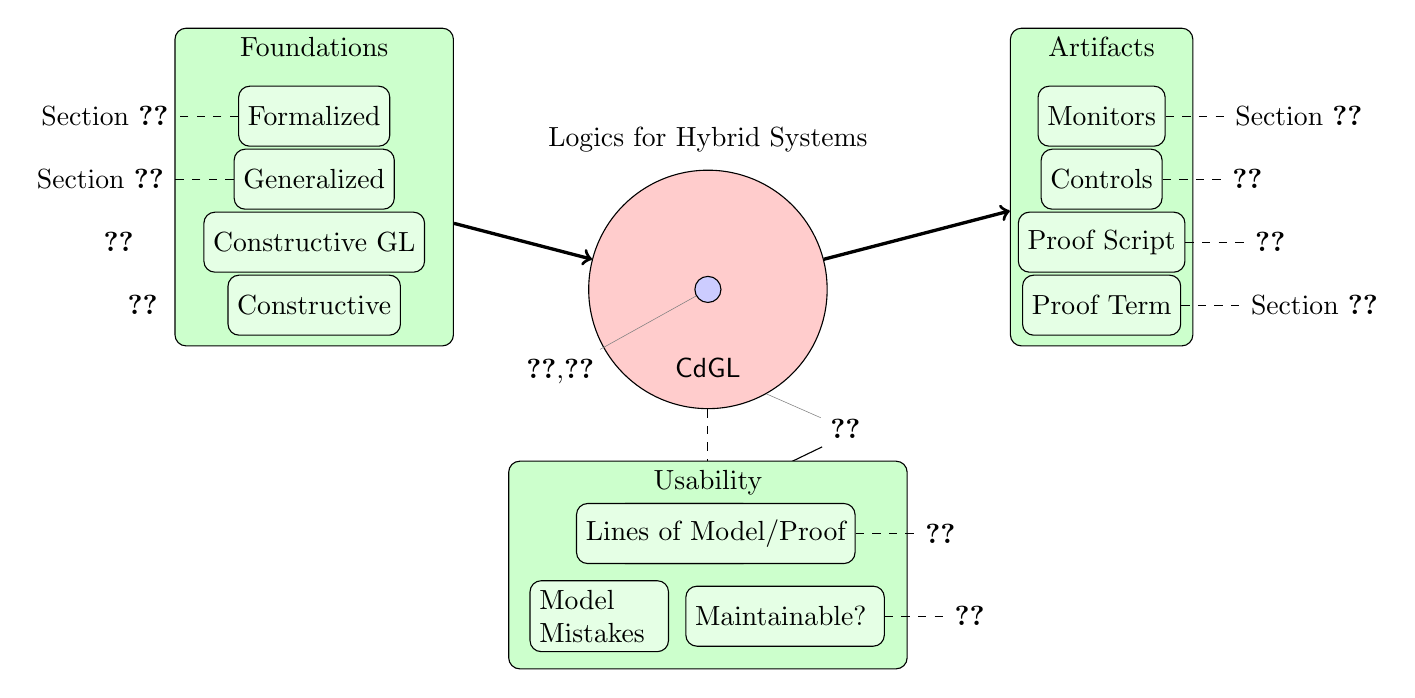
\begin{tikzpicture}
  \draw (0,1.9)  node {Logics for Hybrid Systems};
\draw (0,0)   node[circle]      (CdGLcirc) {\phantom{\hspace{1.1in}}};
\draw (0,-1) node (cdgl) {\phantom{\CdGL}};
\node[coordinate,pin={[pin distance=0.6in]340:{\rref{ch:cdgl}}}] (cdgl-ref) at (cdgl) {};
\draw (0,0)   node[circle, fill=red!20,draw]      (CdGLcirc) {\phantom{\hspace{1.1in}}};
\draw (0,-1) node (cdgl) {\CdGL};
\draw (0,0)   node[circle]  (dl)  {\phantom{\dL}};
\node[coordinate,pin={[pin distance=0.6in]210:{\rref{ch:logical-foundations},\rref{ch:end-to-end-v}}}] (dl-ref) at (dl) {};
\draw (dl) node[circle, fill=blue!20,draw]  {\dL};
\draw (-5, 1.3) node[rectangle,rounded corners,fill=green!20,draw,text depth=1.4in,text width=1.3in,text centered] (logic) {Foundations};
\draw (-5, 2.2) node[rectangle,rounded corners,fill=green!10,draw,thin,minimum height=0.3in] (formalization) {\dL Formalized};
\draw (-5, 1.4) node[rectangle,rounded corners,fill=green!10,draw,thin,minimum height=0.3in] (generalization) {\dL Generalized};
\draw (-5, 0.6) node[rectangle,rounded corners,fill=green!10,draw,thin,minimum height=0.3in] (cgl) {Constructive \GL};
\draw (-5, -0.2) node[rectangle,rounded corners,fill=green!10,draw,thin,minimum height=0.3in] (cdgl) {Constructive \dGL};
\draw node[left=0.3in of formalization] (formal-ref) {\rref{sec:isabelle-fml}};
\draw node[left=0.3in of generalization] (gen-ref) {\rref{sec:definite-description}};
\draw node[left=0.3in of cgl] (cgl-ref) {\rref{ch:cgl}};
\draw node[left=0.3in of cdgl] (cdgl-ref) {\rref{ch:cdgl}};
\draw[dashed] (formalization) -- (formal-ref);
\draw[dashed] (generalization) -- (gen-ref);
\draw (5, 1.3) node[rectangle,rounded corners,fill=green!20,draw,text depth=1.4in,text width=0.82in,text centered] (engine) {Artifacts};
\draw (5, 2.2) node[rectangle,rounded corners,fill=green!10,draw,thin,minimum height=0.3in] (monitors) {Monitors};
\draw (5, 1.4) node[rectangle,rounded corners,fill=green!10,draw,thin,minimum height=0.3in] (controllers) {Controls};
\draw (5, 0.6) node[rectangle,rounded corners,fill=green!10,draw,thin,minimum height=0.3in] (proofscript) {Proof Script};
\draw (5, -0.2) node[rectangle,rounded corners,fill=green!10,draw,thin,minimum height=0.3in] (proofterm) {Proof Term};
\draw node[right=0.3in of monitors] (monitor-ref) {\rref{sec:veriphy}};
\draw node[right=0.3in of controllers] (controllers-ref) {\rref{ch:proofplex}};
\draw node[right=0.3in of proofscript] (proofscript-ref) {\rref{ch:kaisar}};
\draw node[right=0.3in of proofterm] (proofterm-ref) {\rref{sec:veriphy}};
\draw[dashed] (monitors) -- (monitor-ref);
\draw[dashed] (controllers) -- (controllers-ref);
\draw[dashed] (proofscript) -- (proofscript-ref);
\draw[dashed] (proofterm) -- (proofterm-ref);
\node[shape=coordinate] (use-anchor) at (0,-3){};
\draw (1.45,-2) -- (0,-2.7);
\draw (0, -3.5) node[rectangle,rounded corners,fill=green!20,draw,text depth=0.85in,text width=1.9in,text centered] (luser) {Usability};
%\draw (0, -3.1) node[rectangle,rounded corners,fill=green!10,draw,thin,minimum height=0.3in] (monitors)    {Simplicity};
\draw (-0.3, -3.1) node[rectangle,rounded corners,fill=green!10,draw,thin,minimum height=0.3in] (monitors)    {Simplicity};
\draw (0.1, -3.1) node[rectangle,rounded corners,fill=green!10,draw,thin,minimum height=0.3in] (lop)    {Lines of Model/Proof};
%\draw (0, -4.15) node[rectangle,rounded corners,fill=green!10,draw,thin,minimum height=0.3in,text width=0.7in] (controllers) {Modeling Mistakes};
\draw (-1.38, -4.15) node[rectangle,rounded corners,fill=green!10,draw,thin,minimum height=0.3in,text width=0.6in] (modelmistake) {Model Mistakes};
\draw (0.98, -4.15) node[rectangle,rounded corners,fill=green!10,draw,thin,minimum height=0.3in,text width=0.9in] (maintainable) {Maintainable?};
\draw node[right=0.3in of maintainable] (maintain-ref) {\rref{ch:kaisar}};
\draw node[right=0.3in of lop] (lop-ref) {\rref{ch:kaisar}};
\draw[->,very thick] (logic) -- (CdGLcirc);
\draw[->,very thick] (CdGLcirc) -- (engine);
\draw[dashed] (CdGLcirc) -- (luser);
\draw[dashed] (lop) -- (lop-ref);
\draw[dashed] (maintainable) -- (maintain-ref);
\end{tikzpicture}
  \caption{Goals of the thesis}
  \label{fig:goals-diagram}
\end{figure}

\rref{fig:goals-diagram} lays out the relationships between the chapters of the thesis.
The already-completed works in this thesis connect implementation artifacts to foundations by way of \dL:
the monitor synthesis tool \VeriPhy (\rref{sec:veriphy}) connects an implementation (for example, of a robot: \rref{sec:ground-robotics}) to a formal model in \dL.
\rref{ch:logical-foundations} then satisfies the logician by putting \dL (as implemented in \KeYmaeraX) on firm footing in \Isabelle (\rref{sec:isabelle-fml}), and also generalizing the foundations of \dL to survive future development (\rref{sec:definite-description}).
The proposed work extends our logical foundation by developing \CdGL (Constructive \dGL) and Kaisar, a principled language for \CdGL proofs.
We show that this foundation promotes simpler models (\rref{ch:cdgl}) and supports synthesis of both controllers and monitors in the general case.
These additions meet the practical needs of the Engineer and Logic-User while extending the \VeriPhy pipeline on one end to high-level user proofs scripts and rounds out the other end by providing verified controllers, resulting in a stronger safety guarantee than prior versions of \VeriPhy.

At last, we arrive at a concise thesis statement for the thesis as a whole:
\begin{framed}
  \begin{quote}
Constructive Differential Game Logic (\CdGL) enables practical, end-to-end verification of cyber-physical systems.
  \end{quote}
\end{framed}
In \rref{sec:relwork}, we will compare the \CdGL+\VeriPhy approach in detail with other works that follow an end-to-end philosophy.
Our take on end-to-end verification is that results implementation-level guarantees must come via formal guarantees connecting implementation to models, else the Logician will not accept the system as verified.
For this verification to be practical, results should be transported to implementation level automatically, with artifacts that the Engineer can use.
In \rref{sec:ground-robotics}, our realistic 2D ground robotics case study is essential to convince the Engineer that our work scales to realistic scenarios.
The Logic-User must be able to perform their proofs in a high-level, productive language.
Viewed through this lens, \rref{tab:approach-comparison} shows that the \VeriPhy approach, with its strong foundation in logic, marries practical end-to-end verification foundation with rigorous foundations on a level that prior approaches have not.

\section{Related Work}
\label{sec:relwork}
Here, we discuss works that are broadly related to the thesis as a whole.
Works which are relevant primarily to one chapter are discussed in that chapter.


\subsection{Verification of Theorem Provers}
Because theorem-provers are used to ascertain the correctness of critical systems, their own correctness is essential.
This thesis includes a formalization of \dL in \Isabelle (\rref{sec:isabelle-fml}) which has been used to generate a verified proof-term checker for \dL (\rref{sec:veriphy}).
We compare our contributions to other works on theorem prover verification.
In general, the differences among formalizations mirror the differences among the underlying logics, so the unique features of our work include real analysis proofs and an explicit treatment of substitution.

Barras and Werner~\cite{Barras:1997} verified a typechecker for a fragment of Coq in Coq.
Harrison~\cite{Harrison:2006} verified (1) a weaker version of HOL Light's kernel in HOL Light and (2) HOL Light in a stronger variant of HOL Light.
Myreen et al.\ have extended this work, verifying HOL Light in HOL4~\cite{Myreen+Owens+Kumar:2013,Kumar+Arthan+Myreen+Owens:jar:2016} and using their verified compiler CakeML~\cite{DBLP:conf/popl/KumarMNO14} to ensure these guarantees apply at the machine-code level.
Myreen and Davis proved the soundness of the ACL2-like theorem prover Mitawa in HOL4~\cite{Myreen+Davis:itp:2014}.
Anand, Bickford, and Rahli~\cite{DBLP:conf/itp/AnandR14,Rahli+Bickford:cpp:2016}
proved the relative consistency of Nuprl's type theory~\cite{Constable+al:1986,Allen+al:2006} in Coq with the goal of generating a verified prover core.
%
Like the above works, the goal of \rref{sec:isabelle-fml} is to verify the correctness of a theorem prover (\KeYmaeraX).
This goal is one part of the thesis' broader goal of bulletproof foundations: formal proofs are only as trustworthy as their foundations.
Since proof in \dL is a lynchpin of the \VeriPhy approach, it was crucial to show the soundness of \dL's foundations.
%
\rref{sec:isabelle-fml} exposed unique technical challenges because the foundations of \dL differ greatly from those of the other provers.
Soundness for the differential equations of \dL involved significant proofs in real analysis.
The \KeYmaeraX core is based on a uniform substitution calculus, so the formalization also includes significant proofs about substitution.

Our verified checker supports a significant fragment of the \KeYmaeraX core, including enough to recheck proofs of safety for monitor-based synthesized controllers (${\approx}$100K steps).
While the \Isabelle formalization is based directly on the calculus supported in \KeYmaeraX, another contribution of the thesis (\rref{sec:definite-description}) is to develop a foundation for \dL which is more amenable to the practical extensions used in \KeYmaeraX in practice.
Together, these two pieces provide a multifaceted argument how we can trust hybrid systems proofs as done in \KeYmaeraX.
Recently, an independent formalization of classical \dGL has been made~\cite{DBLP:journals/afp/Platzer19}, which emphasizes uniform substitution and simplicity of the formalization over suitability for extraction of a verified checker.

\subsection{Verification of CPS}
%
Hybrid systems verification is a broad and actively studied field.
We discuss some of the major lines of research here.

%\subsubsection{Early Approaches}
%
%\'{A}brah\'{a}m-Mumm et al.\ formalized in PVS~\cite{Mumm+Steffen+Hannemann:iceccs:2001} an
%automaton-based approach similar to timed automata. 
%They implement Floyd's inductive assertion reasoning method.
%However, they only check invariants when transitioning between discrete states, as opposed to our differential invariants which hold continuously.
%Furthermore, they only support continuous dynamics given as explicit solutions.
%Thus they cannot reason by differential invariant, nor can they express systems whose solutions only exist for finite time.
%

\subsubsection{Reachability Analysis}
Model-checking for hybrid systems by reachability analysis is thoroughly studied.
Well-known model-checkers include SpaceEx~\cite{DBLP:conf/cav/FrehseGDCRLRGDM11}, Flow*~\cite{DBLP:conf/cav/ChenAS13}, and C2E2~\cite{DBLP:conf/tacas/DuggiralaMVP15}.
Compared to deductive verification in \dL, the strength of model-checkers is that support a higher degree of automation.
Their downsides typically include a significantly larger trusted base (${\approx}$100,000 SLOC for SpaceEx) and reduced expressivity.
Typical restrictions include restriction to linear differential equations, bounded-time safety, or bounded state spaces.
In a notable exception regarding large trusted cores, \cite{DBLP:conf/tacas/Immler15} verifies a set-based reachability analysis for ODEs in Isabelle using his differential equations library~\cite{DBLP:conf/itp/ImmlerT16}.
While it is trustworthy, it only computes numerical solutions to differential equations, and so cannot handle full hybrid systems nor the symbolic reasoning necessary to show correctness in the general case.
Reachability analysis has been applied to ground robotics~\cite{chen2015benchmark}.

\subsubsection{Differential Dynamic Logics}
This thesis is part of a long line of work using differential dynamic logic (\dL)~\cite{DBLP:journals/jar/Platzer08,DBLP:conf/lics/Platzer12a,DBLP:journals/jar/Platzer17} and logics descended from it.
Compared to reachability analysis approaches, deductive verification in \dL is symbolic and expressive: all polynomial differential equations are supported, and discrete tests and assignments are also polynomial.
Guarantees are typically unbounded-time, and the plant is modeled faithfully as a continuous differential equation, not a discrete difference equation.
The tradeoff is that verification is undecidable, and serious case studies usually require significant manual interaction from the user.
The \KeYmaeraX~\cite{DBLP:conf/cade/FultonMQVP15} theorem prover implements \dL and provides significant automation to minimize the number of interactions required.
\dL and \KeYmaeraX have been applied in a number of case studies~\cite{DBLP:conf/cade/Platzer16}.

This thesis includes a case study which we use to assess \VeriPhy's ability to verify realistic systems.
Our case study generalizes a \dL proofs of 1D straight-line motion (with direct velocity control)~\cite{DBLP:conf/pldi/BohrerTMMP18}, of 2D obstacle avoidance, and 1D liveness~\cite{DBLP:conf/rss/MitschGP13,DBLP:journals/ijrr/MitschGVP17}.
A paper proof of liveness using \dL rules assumed perfect sensing and constant speed \cite{DBLP:journals/corr/abs-1709-02561}.
Their controllers, like ours, are closely related to the classic \textsc{Dynamic-Window}~\cite{DBLP:journals/ram/FoxBT97} control algorithm.
In contrast to the prior \dL effort, we offer stronger results, including 2D liveness, waypoint-following, and end-to-end correctness.

\subsubsection{Synthesis for Planning and Control}
Low-level controllers are an important part of any CPS, so their correctness is an important part of CPS correctness.
Our approach to end-to-end verification (\rref{sec:veriphy}) uses correct-by-construction synthesis of monitors to remove low-level controllers from the trusted base for safety.
However, correctness of controllers is still important to ensure \emph{liveness}, and our case study (\rref{sec:ground-robotics}) assumes high-level plans as an input, while correctness of high-level plans is an interesting problem in its own right~\cite{DBLP:conf/atva/RizaldiISA18}.
In proposed work~(\rref{ch:proofplex}), we will complement our monitor synthesis with correct-by-construction low-level controller synthesis.
Related works have explored planning and control synthesis at the high level, with correctness assumptions on the kinematic models:
\begin{itemize}
\item The tools LTLMoP~\cite{DBLP:conf/iros/FinucaneJK10} and TuLiP~\cite{DBLP:conf/IEEEcca/FilippidisDLOM16} can synthesize robot controls that satisfy a high-level temporal logic specification.
However, they depend on accuracy of their kinematic models, which assume  discrete-space and discrete-time, and the guarantees are not end-to-end.
\item Bisimulation~\cite{871304} is used to synthesize plans based on hybrid dynamics~\cite{DBLP:conf/cdc/BhatiaKV10,DBLP:journals/automatica/FainekosGKP09}, but assumes model compliance and cannot ensure low-level controller correctness.
\item Controllers have been synthesized:
\begin{inparaenum}[\it i)]
\item from temporal logic specifications for linear systems~\cite{DBLP:journals/tac/KloetzerB08},
\item for adaptive cruise control~\cite{DBLP:journals/tcst/NilssonHBCAGOPT16}, tested in simulation and on hardware, and
\item from safety proofs~\cite{DBLP:conf/emsoft/TalyT10} for switched systems using templates,
\end{inparaenum}
\end{itemize}

\subsubsection{Online Verification}
The approaches above are \emph{offline}: i.e., they are used before-the-fact to ascertain the correctness of a hybrid model of a CPS.
In contrast, \emph{online verification} (or runtime verification) uses checks at runtime to enforce correctness.
Online verification excels at treating systems that are not fully understood before runtime (such as sensors and actuators) and systems which we simply wish to not try to fully understand (such as complex untrusted control systems).
However, the guarantees of online verification are weaker and often lack a clear foundation.
\begin{itemize}
\item The basis of online verification is the SIMPLEX~\cite{Krogh1998TheSA} method, which uses a trusted monitor to decide between an untrusted controller and trusted fallback.
\item Runtime reachability analysis has been used for car control~\cite{DBLP:journals/trob/AlthoffD14}, but relies on correctness of the model and of the analysis implementation.
Since reachability tools rely on large, complicated codebases and models are challenging to get right, these assumptions present a correctness gap which stands in the way of an end-to-end argument.
\item \ModelPlex is a tool for synthesizing monitors (for both the controller and plant) from proven-safe \dL models in \KeYmaeraX.
  However, it simply synthesizes a \dL formula describing the monitored conditions, not an executable program.
  Until extensions concurrent with this thesis~\cite{DBLP:journals/corr/abs-1811-06502}, \ModelPlex was also restricted to only hybrid systems whose differential equations have polynomial solutions.
\item High-Assurance SPIRAL~\cite{DBLP:journals/csm/FranchettiLMMGPPKMFJPV17} is a compilation toolchain for \ModelPlex-synthesized monitors for \dL, but does not provide formal end-to-end guarantees, and has not been used to develop an end-to-end system capable of free-range 2D driving.
\item A contribution of this thesis is the \VeriPhy~\cite{DBLP:conf/pldi/BohrerTMMP18} toolchain for \dL.
  \VeriPhy extends SIMPLEX by ensuring the monitor is correct-by-construction (via \ModelPlex), formally proving the safety of the resulting system, and automatically maintaining safety down to machine code implementation.
\end{itemize}


%Ivory \cite{DBLP:conf/haskell/ElliottPWHBSSL15} and Tower \cite{DBLP:conf/plpv/PikeHBEDL14} are used to ensure high-assurance embedded software is memory safe, but do not verify the functional correctness of cyber nor physical behavior.
\subsubsection{End-to-End Approaches}
\label{sec:end-to-end-relwork}
End-to-end verification refers to any verification approach which attempts to verify CPS as they exist in reality while maintaining a rigorous foundation.
Notably, none of these approaches show correctness unconditionally: all have a trusted base and make simplifying assumptions about reality.
\begin{itemize}
\item
  High-Assurance SPIRAL \cite{DBLP:journals/csm/FranchettiLMMGPPKMFJPV17} generates executable x64 machine code based on \dL model.
  However, its claim to ``end-to-end'' status is weaker than that for our tool \VeriPhy, because High-Assurance SPIRAL relies heavily on esoteric compiler optimizations which are difficult to verify correct.
  Moreover, \VeriPhy adopts a deeper understanding of hybrid systems: several stages of \VeriPhy exploit language-level semantic proofs that link the initial hybrid system model to a low-level executable semantics.
  High-Assurance SPIRAL uses only syntactic transformations and does not have a semantic understanding of hybrid system, which precludes the clear connection between the system model and compiled code as provided by \VeriPhy.
\item 
Anand and Knepper~\cite{DBLP:conf/itp/AnandK15} developed the framework ROSCoq based on the Logic of Events for reasoning about distributed CPS in Coq with constructive reals and generating verified controllers.
Their use of constructive reals is prescient, and inspires the design choices in \rref{ch:proofplex}.
However, they provide limited support for reasoning about derivatives, requiring extensive manual proofs by the user.
They do not synthesize and automatically verify monitors, nor is their machine code verified.
\item 
VeriDrone by Ricketts et al.~\cite{Ricketts:memcode:2015} is a framework for verifying hybrid systems in Coq that relies on a discrete-time temporal logic called RTLA, inspired by TLA~\cite{Lamport:hybrid:1992}.
They prove an analog of DI, but not the other ODE axioms, thus other ODE proofs, as well as arithmetic proofs, are likely laborious.
They do not automatically verify monitors, nor is their machine code verified.
Their use of discrete-time temporal logic also raises foundational concerns, since real time is best understood as continuous.
\end{itemize}



%  We provide a simpler model which enabled LEEV of our implementations with \VeriPhy, whereas the model of~\cite{DBLP:journals/ijrr/MitschGVP17} is too restrictive (i.e., the synthesized monitor would always fail in practice).
%\item Reachability is most-often used in design, but can also be used for model-predictive control~\cite{Bemporad2000PerformanceDR}.
%Hybrid systems theorem-proving in \dL~\cite{DBLP:books/sp/Platzer18} with \KeYmaeraX~\cite{DBLP:conf/cade/FultonMQVP15} is typically less automated, with unique advantages in system complexity (polynomial ODEs), property complexity (unbounded-time safety and liveness), and rigor (small\cite{DBLP:conf/cade/FultonMQVP15}, verified~\cite{DBLP:conf/cpp/BohrerRVVP17} trusted base).  Control strategies for ground vehicles are well-studied.
%Reachability for liveness has been investigated~\cite{BEMPORAD2001382}.



\chapter{Background: Differential Game Logic \dGL}
\emph{Differential dynamic logic} (\dL)~\cite{DBLP:books/sp/Platzer18,DBLP:journals/jar/Platzer08,DBLP:journals/jar/Platzer17,DBLP:conf/lics/Platzer12b:TR} is a dynamic logic for the formal verification of hybrid systems, which combine discrete transitions with differential equations to model CPSs.
\emph{Differential game logic} (\dGL)~\cite{DBLP:journals/tocl/Platzer15,DBLP:journals/tocl/Platzer17,DBLP:conf/cade/Platzer18} extends the programs $\alpha$ of \dL with a turn-taking operator $\pdual{\alpha}$ to enable representing and verifying hybrid \emph{games} which extend hybrid systems with \emph{adversarial} dynamics.

While the already-completed thesis chapters (\rref{ch:logical-foundations}, \rref{sec:veriphy}) employ \dL, we present full \dGL since 
\begin{inparaenum}[i)]
  \item the proposed works (\rref{ch:cdgl},\rref{ch:proofplex}) will require an understanding of full \dGL, and
  \item an introductory understanding of \dGL will also provide an introductory understanding of \dL.
\end{inparaenum}
While the syntax of \dGL and \dL are nearly identical, their semantic differences are deep: \dL is a regular modal logic whose denotational semantics can be and are given in the forward-chaining, relational Kripke style, while \dGL is a subregular logic with a backward-chaining winning-region semantics.

\section{Syntax}
\label{sec:dgl-syntax}
We introduce the syntax and informal meaning of \dGL here, then introduce the winning-region semantics formally in \rref{sec:dgl-semantics}.
The syntax of \dGL consists of three syntactic classes: terms, formulas, and hybrid games.

\begin{definition}[Terms of \dGL]
Terms $\theta, \eta$ of \dGL are defined recursively according to the following grammar:
\[\theta,\eta \bebecomes q \alternative x \alternative \theta + \eta \alternative \theta \cdot \eta \alternative \der{\theta} \]
\end{definition}
Where $q \in \mathbb{Q}$ is a rational constant, $x \in \allvars$ is a program variable and $\allvars$ is the (at most countable) set of all base variable names.
For every base variable $x \in \allvars,$ there is a differential variable $\D{x} \in \D{\allvars}$ standing for the differential of $x$.
Terms $\theta + \eta$ and $\theta \cdot \eta$ are the sum and product of $\theta$ and $\eta,$ and $\der{\theta}$ is the \emph{differential} of term $\theta$.
It is worth noting that the \dGL term language is restrictive, and for good reason: all terms are polynomials, so all terms are defined in every state and even $C^\infty$-smooth.
Because \dGL terms are well-behaved, the theory of \dGL is simplified as a result.
In \rref{sec:definite-description}, we show how to remove these simplifying assumptions in the context of \dL, enabling many more term constructs that are essential in practical proving, the most common constructs including quotients, roots, trigonometric functions, and conditionals.


\begin{definition}[Formulas of \dGL]
  Formulas are defined by the following grammar:
\[\phi,\psi \bebecomes \theta \sim \eta \alternative \phi \land \psi \alternative \phi \lor \psi \alternative \neg \phi \alternative \phi \limply \psi \alternative \phi \lequiv \psi \alternative \lforall{x}{\phi} \alternative \lexists{x}{\phi} \alternative \dbox{\alpha}{\phi} \alternative \ddiamond{\alpha}{\phi}\]
\end{definition}
where $\sim$ stands for any comparison operator $\sim \in \{\leq, <, =, \neq, >, \geq\}$.
We write conjunctions $\phi \land \psi,$ negations $\phi \lor \psi,$ disjunctions $\phi \lor \psi,$ implications $\phi \limply \psi,$ biimplications $\phi \lequiv \psi$, and quantifiers over real numbers $\lexists{x}{\phi}$ and $\lforall{x}{\phi}$.
The diamond modality $\ddiamond{\alpha}{\phi}$ says that the player who is actively making decisions (typically named Angel) has a strategy for the game $\alpha$ which ensures postcondition $\phi$.
The box modality $\dbox{\alpha}{\phi}$ says that the player who is not currently making decisions (typically named Demon) has a strategy for the game $\alpha$ which ensures postcondition $\phi$.
Because \dGL is a classical logic, it is worth noting that the formula syntax is not minimal: many constructs such as implication, equivalence, disjunction, universal quantifiers, and the box modality are all definable classically.
This will not be the case in the proposed logic \CdGL (\rref{ch:cgl}) since some of the definitions are valid only classical, not constructively.

\begin{definition}[Hybrid games]
Games are defined by the following grammar:  
\[\alpha,\beta \bebecomes \pevolvein{\D{x}=\theta}{\ivr} \alternative \humod{x}{\theta} \alternative \prandom{\alpha} \alternative \ptest{\phi} \alternative \pchoice{\alpha}{\beta} \alternative \alpha;~\beta \alternative \prepeat{\alpha} \alternative \pdual{\alpha}\]
\end{definition} 
where $\humod{x}{\theta}$ stores the current value of term $\theta$ in program variable $x$  and test $\ptest{\phi}$ makes Angel lose if formula $\phi$ does not hold in the current state.
In nondeterministic assignment $\prandom{x},$ Angel chooses a value $r \in \mathbb{R}$ to assign to $x$.
Program $\pevolvein{\D{x}=\theta}{\phi}$ evolves $x$ continuously according to the differential equation (ODE) $\D{x}=\theta$ for a duration $d \geq 0$ of Angel's choosing, but Angel must ensure that $\phi$ is true throughout the evolution of $\D{x}=\theta,$ else they lose.
In game $\pchoice{\alpha}{\beta},$ Angel chooses whether to play game $\alpha$ or game $\beta$.
In game $\alpha;~\beta$ the players must first play $\alpha$ and then play $\beta$; this case is largely responsible for the need to employ backward-chaining semantics in \dGL, as it is most natural to first ask from what region $X$ is there a winning strategy for $\beta$, then ask from what region does Angel have a strategy to reach $X$ when playing $\alpha$.
In the iterated game $\prepeat{\alpha}$, Angel decides at the end of each loop iteration whether to continue playing $\alpha$ another time.
All plays must be finite (Angel must stop eventually), but Angel need not decide a-priori \emph{when} to stop, let alone announce that decision to Demon beforehand.
If Angel cannot reach the goal region without repeating $\alpha$ infinitely, then Angel loses.
To play the dual game $\pdual{\alpha},$ Angel and Demon switch roles then play game $\alpha$ in their new roles.
That is, the player previously known as Demon makes the decisions in $\alpha,$ at least until another dual operator is encountered.
We parenthesize hybrid games $\{ \alpha \}$ for clarity and disambiguation as needed.
We will sometimes speak of \emph{demonic} loops, choices, etc., which are derived from the angelic forms as follows:
\begin{align*}
\alpha^\times &\equiv \{\prepeat{\{{\alpha{}\pdual{}}\}}\}{\pdual{}}                 & \pdual{\ptest{\phi}}      &\equiv \pdual{\{\ptest{\phi}\}}\\
\alpha \cap \beta  &\equiv \left\{\pdual{\alpha} \cup \pdual{\beta}\right\}\pdual{} & \pdual{\pevolvein{\D{x}=\theta}{\psi}} &\equiv \pdual{\{\pevolvein{\D{x}=\theta}{\psi}\}}\\
\pdual{\humod{x}{\theta}} &\equiv \humod{x}{\theta}                                      & \pdual{\{\alpha;~\beta\}} &\equiv \pdual{\alpha};~\pdual{\beta} 
\end{align*}
In a Demonic test, Demon controls \emph{only} the duration of the loop, then returns control to Angel during the body.
Likewise, Demon controls only which branch is taken in a demonic choice.
In Demonic tests and differential equations, Demon is responsible for passing the test or satisfying the domain constraint.
In the latter, Demon also chooses the duration.
Deterministic assignment and sequential competition are self-dual, so their Demonic forms are identical to the Angelic.




We now give an example hybrid game and example safety and liveness properties.
The game in \rref{ex:driving-game} is a generalization of a standard hybrid systems model to a hybrid game.
\begin{example}[Acceleration-Controlled 1D Driving]
\label{ex:driving-game}
\begin{align}
\alpha_\times\equiv&\\
\label{eq:driving-init}\humod{v}{0};~&\humod{x}{0};\pdual{(\prandom{\obsvar};\prandom{T};\prandom{A};\prandom{B}; \ptest{\obsvar > 0 \land T > 0 \land A > 0 \land B > 0})};\\
\label{eq:driving-angel}\big\{ &\prandom{a};~\ptest{-B \leq a \land a \leq A};\\ 
\label{eq:driving-demon}       &\pdual{\humod{t}{0};~\{\pevolvein{\D{x}=v, \D{v}=a, \D{t}=1}{t \leq T \land v \geq 0}\}}\big\}^\times
\end{align}
\end{example}
The first line \rref{eq:driving-init} is an initialization phase: we (Angel) call the current position $x = 0$ and are initially stopped ($v = 0$).
The opponent then picks how far away our obstacle (\obsvar) is and how long Angel will have to wait between control decisions ($T$).
They also pick Angel's maximum braking rate $B$ and maximum acceleration rate $A$.
One could argue on principle that neither player really picks the timestep $T,$ in practice this is determined by the speed of the robot's processors, sensors, and actuators, as well as the speed of its control program.
However, what's important is that robot's controller (the Angel player) is \emph{not} the one who picks, so a conservative model should assume the worst, which is that their opponent (the environment) gets to pick.
The same goes for the rates $A$ and $B$.
It would also be eminently unreasonable if the obstacle already collided with the robot at the start of the game, and would be nonsensical if the control cycle lasted zero time or less, or if the robot could not accelerate or brake, thus the environment is responsible for picking positive $\obsvar, \Tvar, \Avar$, and  $\Bvar,$ else they lose by default and Angel wins immediately.
The remainder of the game is a demonic loop $\alpha^\times$ where the Demon player controls the duration.
Angel's turn consists of making a control decision by setting the acceleration $a$.
Angel has near complete freedom to set the acceleration: they may set any value ($\prandom{a}$) so long as it is within the physical limits of the car ($\ptest{-B \leq a \land a \leq A}$).
It is Angel's responsibility to do so, and they lose the game if the acceleration is out of bounds.
Next, the car moves according to ideal Newtonian physics: the velocity $v$ continuously changes according to acceleration $a$ while position changes continuously according to the velocity.
Demon (the environment) controls the duration of the ODE, but is constrained to the timestep $t \leq T$: i.e., Angel's control action must be safe even if Demon chooses not to use the full time budget, but need not be safe past time $T:$ in that case Demon is responsible for breaking the rules, so Angel wins.
The equation $\D{t}=1$ simply says that $t$ represents the time elapsed in the current ODE run.
The remainder of the game is a \emph{demonic loop} $\alpha^\times$ where the Demon player controls the duration.
We also write $\alpha_*$ for $\alpha_\times$ with an Angelic loop.

We give examples of safety and liveness theorems:
\begin{example}[1D Driving Game Safety and Liveness]
  \begin{align*}
    \textit{safe} &\equiv \ddiamond{\alpha_\times}{\xvar \leq \obsvar}\\
    \textit{live} &\equiv \ddiamond{\alpha_*}{\left(\xvar \geq \obsvar \lor t \leq \frac{T}{2}\right)}
  \end{align*}
\end{example}
The safety theorem \emph{safe} says that Angel (the robot) has a strategy to ensure $\xvar \leq \obsvar$ (i.e. a strategy not to hit the obstacle) regardless how long Demon runs the loop and the ODE.
The liveness theorem \emph{live} says that Angel (the robot) has a strategy to reach the obstacle, \emph{so long as} Demon always runs the ODE long enough ($t \geq \frac{T}{2}$).
The requirement on running the ODE long enough is to rule out \emph{Zeno} behaviors by Demon: without this restriction, Demon can run the ODE for shorter and shorter durations, with infinitely many iterations in finite time, which is not physically realizable but would falsify the liveness theorem.

It is worth noting that prior case studies ~\cite{DBLP:conf/emsoft/JeanninGKGSZP15,DBLP:conf/fm/LoosPN11,DBLP:conf/rss/MitschGP13,DBLP:conf/hybrid/PlatzerQ08} used vanilla \dL for hybrid \emph{systems} in \KeYmaeraX (\rref{sec:veriphy},\rref{sec:ground-robotics}).
In \rref{ch:cdgl} of this thesis, we will advocate for making (constructive) games proofs the standard.
We foreshadow the motivations of \rref{ch:cdgl} here.

Consider a hybrid \emph{system} version of \rref{ex:driving-game}:
\begin{example}[Acceleration-Controlled 1D Driving System]
\label{ex:driving-system}
\begin{align}
\label{eq:driving-sys-pre}
\textrm{Pre}      & \equiv v=0 \land x=0 \land \obsvar > 0 \land T > 0 \land A > 0 \land B > 0\\
\alpha_{\textrm{Sys}}& \equiv\\
\label{eq:driving-sys-forward}\big\{\big\{~&\prandom{a};~\ptest{-B \leq a \land a \leq A};~\ptest{\frac{(v+a T)^2}{2\Bvar} \leq \obsvar - \left(\xvar + \vvar \Tvar + \avar\frac{\Tvar^2}{2}\right)}\\
\label{eq:driving-sys-stay}     \cup&~\ptest{v = 0};~\humod{a}{0}\\
\label{eq:driving-sys-brake}    \cup&~\ptest{v \geq 0};~\humod{a}{-B}\big\};\\
\label{eq:driving-sys-demon}       &\{\pevolvein{\D{x}=v, \D{v}=a, \D{t}=1}{t \leq T \land v \geq 0}\}\big\}^*
\end{align}
\end{example}
Note $\alpha_{\text{Sys}}$ of \rref{ex:driving-system} is much more complex and explicit than \rref{ex:driving-game}.
This is because the \emph{strategy} by which acceleration is chosen must be explicitly given in the model as three cases:
\rref{eq:driving-sys-forward} allows any physically-possible choice that is safe for time $\Tvar,$ \rref{eq:driving-sys-stay} lets a robot stay stopped, and \rref{eq:driving-sys-brake} allows braking.

Why are \rref{ex:driving-game} and game models in general simpler? % $\alpha_{\textrm{Sys}}$ so much longer than 
A typical game model has shape $\prepeat{(\pdual{\ctrl};~\plant)},$ where the turn-taking (or dual) operator $\pdual{\alpha}$ has the affect of alternating between the modalities $\ddiamond{\alpha}{\phi}$ and $\dbox{\alpha}{\phi}$.
Most often, we wish to show that there \emph{exists} a control choice where \emph{all} behaviors of the environment are safe and live, and so on for all iterations of the system.
Such iterated modality alterations are precisely the one pattern expressible in \dGL but not \dL~\cite{DBLP:journals/tocl/Platzer15}.
In vanilla \dL, safety is usually expressed in the form $\phi \limply \dbox{\prepeat{(\ctrl;~\plant)}}{\psi}$ and liveness is approximated as
$\phi \limply \ddiamond{\prepeat{(\ctrl;~\plant)}}{\psi}$ or $\phi \limply \dbox{\prepeat{(\ctrl;~\plant)}}{\ddiamond{\prepeat{(\ctrl;~\plant)}}{\psi}}$.
\dGL models are simpler because in typical \dL usage, \emph{all} cases of a controller must be safe, whereas a safe choice need only \emph{exist} in a game.
As a result, operational information (what control decision is made in which circumstances) is present in \dL models, whereas it need only appear in \emph{proofs} in \dGL.

As discussed further in \rref{ch:cdgl}, relegating control choices to the proof has advantages for synthesis in \CdGL as well as simplicity advantages.
That being said, the maturity of \KeYmaeraX and the many available case studies show the utility of the thesis chapters which target vanilla \dL as well.
The connections between vanilla \dL and \CdGL will be further discussed in \rref{ch:cdgl}.

\section{Semantics}
\label{sec:dgl-semantics}
We give the denotational semantics for classical hybrid game logic \dGL, which is divided into a semantics for terms, formulas, and games.
Throughout the semantics, states are written $\omega, \nu, \mu : \allstate$ where the set of states $\allstate$ is in bijection to $\mathbb{R}^n$ for $n = \abs{\allvars \cup \D{\allvars}}$ where $\allvars$ is the set of base variables and $\D{\allvars}$ the set of differential variables.
Regions are sets of states and are ranged over by $X, Y, Z$.

\begin{definition}[Classical term semantics]\label{def:dgl-sem-term}
The semantics of a term $\tint{\theta}{\om} : \mathbb{R}$ is the value of term $\theta$ in state $\om$, and is defined inductively on $\theta$:

\begin{minipage}{0.5\textwidth}
\begin{align*}
  \tint{q}{\om} &= q      & \tint{\theta + \eta}{\om}     &= \tint{\theta}{\om} + \tint{\eta}{\om}   \\
  \tint{x}{\om} &= \om(x) & \tint{\theta \cdot \eta}{\om} &= \tint{\theta}{\om} \cdot \tint{\eta}{\om}
\end{align*}
\end{minipage}
\begin{minipage}{0.5\textwidth}
${\tint{\der{\theta}}{\om} = \sum_{x \in \allvars} \frac{\partial \tint{\theta}{\om}}{\partial x} \cdot \omega(\D{x})}$
\end{minipage}
%\begin{minipage}{0.5\textwidth}
%\begin{align*}
%  \tint{q}{\om} &= q      & \tint{\theta + \eta}{\om}     &= \tint{\theta}{\om} + \tint{\eta}{\om}       & \tint{\der{\theta}}{\om}&= \sum_{x \in \allvars} \frac{\partial \tint{\theta}{\om}}{\partial x} \cdot \omega(\D{x})\\
%  \tint{x}{\om} &= \om(x) & \tint{\theta \cdot \eta}{\om} &= \tint{\theta}{\om} \cdot \tint{\eta}{\om}   & &
%\end{align*}
\end{definition}
That is, literals denote themselves, variables $x$ take their meaning from the state $\om,$ sums and products denote the sum and product of the denotation of their operands respectively, and the differential $\der{\theta}$ denotes the sum of every partial derivative of the denotation of $\theta,$ each scaled by the value of the corresponding differential variable $\D{x}$.
Because every term mentions at most a finite number of variables and the partial with respect to an unmentioned variable is uniformly zero, this sum always has finite support.
An advantage of this semantics is that it is defined in every state while agreeing with the intuitive meaning of ``time derivative of $\tint{\theta}{\om}$'' whenever a differential appears in the postcondition of an ODE.

\begin{definition}[Classical formula semantics]\label{def:dgl-sem-fml}
The semantics of a formula $\phi$ is given by the relation $\fint{\phi}{\om},$ which is defined inductively on $\phi$
\begin{align*}
\fint{\theta \sim \eta}  &= \{\om~|~\tint{\theta}{\om} \sim \tint{\eta}{\om}\} && \text{ for }\sim \in \{\leq,<,=,\neq,>,\geq\}\\
\fint{\neg \phi}         &= \fint{\phi}^C && \\
\fint{\phi \land \psi}   &= \fint{\phi}{\om} \cap \fint{\psi}{\om}\\
\fint{\phi \limply \psi} &= \{\om~|~ \om \in \fint{\phi}{\om} \text{ implies } \om \in \fint{\psi}\}\\
\fint{\phi \lequiv \psi} &= \{\om~|~ \om \in \fint{\phi}{\om} \text{ iff } \om \in \fint{\psi}\}\\
\fint{\lexists{x}{\phi}} &= \{\om~|~ \subst[\om]{x}{r} \in \fint{\phi}\} && \text{ for some }x \in \mathbb{R}\\
\fint{\lforall{x}{\phi}} &= \{\om~|~ \subst[\om]{x}{r} \in \fint{\phi}\} && \text{ for all }x \in \mathbb{R}\\
\fint{\ddiamond{\alpha}{\phi}} &=  \strategyfor[\alpha]{\fint{\phi}}\\
\fint{\dbox{\alpha}{\phi}} &= \dstrategyfor[\alpha]{\fint{\phi}}
\end{align*}
where $\strategyfor[\alpha]{X}$ and $\dstrategyfor[\alpha]{X}$ are the regions from which Angel (or Demon, respectively) has a strategy to reach a region $X$.
\end{definition}

\begin{definition}[Classical game semantics]\label{def:dgl-sem-game}
For any game $\alpha$ and goal region $X \subseteq \allstate$, we inductively define the \emph{winning region} $\strategyfor[\alpha]{X}$ for Angel, i.e., the region from which they have a strategy to enter region $X$ after playing game $\alpha$:
\begin{align*}
\strategyfor[\humod{x}{\theta}]{X} &= \{ \om \in \allstate~|~\subst[\om]{x}{\tint{\theta}{\om}}\} \\
\strategyfor[\prandom{x}]{X}       &= \{ \om \in \allstate~|~\subst[\om]{r}{\tint{\theta}{\om}}\text{ for some }r \in \mathbb{R}\} \\
\strategyfor[\pevolvein{\D{x}=\theta}{\ivr}]{X} &= \{\varphi(0) \in \allstate~|~\varphi(r) \in X\text{ for some }r \in \mathbb{R}_{\geq0}\text{ and (differentiable) }\varphi:[0,r]\to \allstate\\
&\text{ such that }\varphi(\zeta) \in \fint{\ivr}\text{ and } \frac{\partial \varphi(t)(x)}{\partial t}(\zeta) = \tint{\theta}{\varphi(\zeta)}\text{ for all }0 \leq \zeta \leq r \}\\
\strategyfor[\ptest{\phi}]{X}      &= \fint{\phi} \cap X \\
\strategyfor[\alpha \cup \beta]{X} &= \strategyfor[\alpha]{X} \cup \strategyfor[\beta]{X}\\
\strategyfor[\alpha;\beta]{X}      &= \strategyfor[\alpha]{\strategyfor[\beta]{X}}\\
\strategyfor[\prepeat{\alpha}]{X}  &= \bigcap\{Z \subseteq \allstate~|~ X \cup \strategyfor[\alpha]{Z} \subseteq Z\}\\
\strategyfor[\pdual{\alpha}]{X}    &= (\strategyfor[\alpha]{X^C})^C
\end{align*}
Likewise, we define the winning regions $\dstrategyfor[\alpha]{X}$ for \emph{Demon}, which are dual to those for Angel:
\begin{align*}
\dstrategyfor[\humod{x}{\theta}]{X} &= \{ \om \in \allstate~|~\subst[\om]{x}{\tint{\theta}{\om}}\}\\
\dstrategyfor[\prandom{x}]{X}       &= \{ \om \in \allstate~|~\subst[\om]{r}{\tint{\theta}{\om}}\text{ for all }r \in \mathbb{R}\} \\
\dstrategyfor[\pevolvein{\D{x}=\theta}{\ivr}]{X} &= \{\varphi(0) \in \allstate~|~\varphi(r) \in X\text{ for all }r \in \mathbb{R}_{\geq0}\text{ and (differentiable) }\varphi:[0,r]\to\allstate\\
&\text{ such that }\varphi(\zeta) \in \fint{\ivr}\text{ and }\frac{\partial\varphi(t)(x)}{\partial t}(\zeta) = \tint{\theta}{\varphi(\zeta)\text{ for all }0 \leq \zeta \leq r}\}\\
\dstrategyfor[\ptest{\phi}]{X}         &= (\fint{\phi})^C \cup X\\
\dstrategyfor[\alpha\cup\beta]{X}   &= \dstrategyfor[\alpha]{X} \cap \dstrategyfor[\beta]{X}\\
\dstrategyfor[\alpha;\beta]{X}      &=  \dstrategyfor[\alpha]{\dstrategyfor[\beta]{X}}\\
\dstrategyfor[\prepeat{\alpha}]{X}  &= \bigcup\{Z \subseteq \allstate~|~ Z \subseteq X \cap \dstrategyfor[\alpha]{Z}\}\\
\dstrategyfor[\pdual{\alpha}]{X}    &= (\dstrategyfor[\alpha]{X^C})^C
\end{align*}
\end{definition}
Note that this winning-region semantics is backward-chaining, which corresponds to the construction of winning regions by \emph{backward induction} in game theory.
The semantics are backward-chaining in the sense that we first commit to a goal region $X,$ from which we can construct an winning region containing the winning \emph{initial} states.
This is in contrast to \dL~\cite{DBLP:books/sp/Platzer18} and \CGL (\rref{ch:cgl}), both of which have a forward-chaining Kripke-style presentation, where the final region is constructed for a given initial region.

%\strategyfor{}{}
%\dstrategyfor{}{}
\section{Proof Calculus}
We recite the proof calculus for \dGL in \rref{fig:dgl-axioms}.
The proof calculus is given as a Hilbert system: axioms are repeatedly applied to recursively decompose hybrid games.
While many basic axioms are the same in \dL and \dGL, some are necessarily different because \dGL is subregular: for example, Kripke's axiom K fails in \dGL and is in practice subsumed by \irref{dglMon}.

\begin{figure}
  \centering
  \begin{calculuscollections}{\columnwidth}
    \begin{calculus}
\cinferenceRule[dglbox|{$[\cdot]$}]{}
{
\linferenceRule[equiv]{\dbox{\alpha}{\phi}}{\neg\ddiamond{\alpha}{\neg\phi}}
}{}
\cinferenceRule[dglassign|{$\langle:=\rangle$}]{}
{
\linferenceRule[equiv]{\ddiamond{\humod{x}{\theta}}{\phi(x)}}{\phi(\theta)}
}{}
\cinferenceRule[dglrandom|{$\langle{:}*\rangle$}]{}
{
\linferenceRule[equiv]{\ddiamond{\humod{x}{\theta}}{\phi(x)}}{\lexists{x}{\phi(x)}}
}{}
%\begin{figure}
%  \centering
%  \begin{calculuscollections}{\columnwidth}
%    \begin{calculus}
\cinferenceRule[dglsolve|{$\langle'\rangle$}]{$\D{y}(t)=\theta$}
{
\linferenceRule[equiv]{\ddiamond{\pevolve{\D{x}=\theta}}{\phi}}{\lexists{t{\geq}0}{\ddiamond{\humod{x}{y(t)}}{\phi}}}
}{}
\cinferenceRule[dgltest|{$\langle?\rangle$}]{}
{
\linferenceRule[equiv]{\ddiamond{\ptest{\psi}}{\phi}}{(\phi \land \psi)}
}{}
\cinferenceRule[dglchoice|{$\langle\cup\rangle$}]{}
{
\linferenceRule[equiv]{\ddiamond{\alpha \cup \beta}{\phi}}{\ddiamond{\alpha}{\phi} \lor \ddiamond{\beta}{\phi}}
}{}
\cinferenceRule[dglcompose|{$\langle;\rangle$}]{}
{
\linferenceRule[equiv]{\ddiamond{\alpha;\beta}{\phi}}{\ddiamond{\alpha}{\ddiamond{\beta}{\phi}}}
}{}
\cinferenceRule[dgliter|{$\langle*\rangle$}]{}
{
\linferenceRule[impl]{\phi\lor\ddiamond{\alpha}{\ddiamond{\prepeat{\alpha}}{\phi}}}{\ddiamond{\prepeat{\alpha}}{\phi}}
}{}
\cinferenceRule[dgldual|{$\langle{}^d\rangle$}]{}
{
\linferenceRule[equiv]{\ddiamond{\pdual{\alpha}}{\phi}}{\neg\ddiamond{\alpha}{\neg\phi}}
}{}
\cinferenceRule[dglMon|M]{}
{
\linferenceRule[formula]{\phi\limply\psi}{\ddiamond{\alpha}{\phi}\limply\ddiamond{\alpha}{\psi}}
}{}
\cinferenceRule[dglfixpoint|FP]{}
{
\linferenceRule[formula]{\phi\lor\ddiamond{\alpha}{\psi} \limply \psi}{\ddiamond{\prepeat{\alpha}}{\phi} \to \psi}
}{}
    \end{calculus}
  \end{calculuscollections}
  \caption{Selected axioms and rules for \dGL}
  \label{fig:dgl-axioms}
\end{figure}
We first discuss the individual axioms, then discuss how the axioms are used together in proofs.
Axiom \irref{dglbox} says that the modalities $\ddiamond{\alpha}{\phi}$ and $\dbox{\alpha}{\phi}$ are dual to each other for arbitrary games $\alpha,$ whereas the axiom \irref{dgldual} says game 
$\pdual{\alpha}$ is dual to $\alpha$.
In practical proofs it is often easier to say that the $\pdual{\alpha}$ operation switches players and then plays $\alpha,$ as in the derived axiom:
\[
\cinferenceRule[dglSwitch|${\langle\cdot\rangle}^d$]{}
{
\ddiamond{\pdual{\alpha}}{\phi} \lequiv \dbox{\alpha}{\phi}
}{}\]
Axiom \irref{dglassign} says assignments can be eliminated by substituting in the postcondition, while \irref{dglrandom} says random assignments can be converted to quantifiers.
Axiom \irref{dglsolve} says that if there exists a function $y(t)$ which solves an ODE, then the ODE can be eliminated by substituting in $y(t)$.
This axiom gives the case where there is no domain constraint because ODEs with domain constraints are derivable from those without them.
The practicality of this axiom depends on the complexity of $y(t)$. 
Especially when $y(t)$ is not a polynomial, it is preferable to reason with \emph{differential invariants}~\cite{DBLP:books/sp/Platzer18}.
Axiom \irref{dgltest} says a test passes when the test condition holds.
Axiom \irref{dglchoice} says Angel chooses which game to play.
Axiom \irref{dglcompose} says game $\alpha;\beta$ is played by playing $\alpha$ first, then $\beta$ in the resulting state.
Axiom \irref{dgliter} says a repetition game can be played by choosing between playing zero rounds or playing some strategy for the first round followed by some strategy for the repetition.
Axiom \irref{dglMon} says hybrid games satisfy monotonicity.
Axiom \irref{dglfixpoint} says repetition $\prepeat{\alpha}$ is a fixpoint of $\alpha$.

In practice, \dGL proofs are done in a backward-chaining style by decomposing goal formulas.
To this end, \KeYmaeraX implements \dGL as a sequent-calculus, whose rules are interderivable with the Hilbert-style axioms in \rref{fig:dgl-axioms}.
Many constructs, such as tests, sequential compositions, choices, and deterministic assignments, can be decomposed without any special insight because there is a single canonical introduction or elimination rule.
Human insight is required to supply invariants for loops and differential equations, and when instantiating first-order quantifiers, or equivalently non-deterministic assignments.

Once the game has been decomposed, the remaining goals are typically first-order logic over the reals.
While this fragment of \dGL is decidable in theory, it has doubly-exponential complexity~\cite{Davenport1988}, and so human insight is necessary in practice.
In addition to instantiating quantifiers, typical interactive methods include weakening unnecessary assumptions, simplifying away arithmetic terms whose details are not needed for the proof, or applying a valid axiom of real arithmetic.

\chapter{Completed Work:  Logical Foundations}
\label{ch:logical-foundations}
A bulletproof theoretical foundation is essential to our approach to end-to-end verification, as it allows the Logician to conclude that our models are fully understoood and our proofs sound.
Logics for verification of hybrid systems and hybrid games are the main formal tool with which we wish to develop correct CPS's, and as such it is doubly important that the logics themselves are developed with the absolute highest degree of certainty in their correctness.
In this chapter, we discuss two completed works by the author.
These works not only attest that an adequate theoretical foundation has been laid for the remaining chapters of the thesis, but also that the author is adequately experienced with developing logical foundations for the proposed works to succeed.

\section{Formalization of \dL in \Isabelle}
\label{sec:isabelle-fml}
When we perform proofs in \dL (or likewise in \dGL), the Logician wishes to know that the theorem we believe we have proved is indeed true.
This property is called soundness, and paper proofs of soundness are provided in the papers which developed a sequent calculus~\cite{DBLP:journals/jar/Platzer08} and uniform substitution~\cite{DBLP:journals/jar/Platzer17} calculus for \dL, of which the latter is the basis for the implementation of \dL in the theorem prover \KeYmaeraX~\cite{DBLP:conf/cade/FultonMQVP15}.
However, proofs on paper are notoriously susceptible both to
\begin{inparaenum}[i)]
  \item soundness errors by human logical blunder and
  \item even more often, completeness errors by omission: 
    paper proofs often focus on the simplest cases of the proof, providing no evidence that the implementation will continue to be correct in the most difficult cases, exactly when it is most in need of formal assurance.
\end{inparaenum}
Errors of both kinds can be most robustly addressed by formalizing the entire development of the proof system in a general-purpose proof assistant such as Isabelle~\cite{ISABELLE} or Coq~\cite{COQ}, starting from syntax and semantics up to axioms and ultimately a soundness theorem for an entire proof-checking procedure.
Errors of the first kind are the easiest to address: assuming we have not accidentally exploited a bug in the host prover, an erroneous logical step in the mechanized proof will simply be rejected by the prover.
To totally eliminate errors of the second kind requires a more ambitious effort: once we have formalized \dL in another prover, how do we know that we have formalized every important feature and that we have not forgotten one?
After all, if we forget to include a certain feature in our paper proof, we might very easily forget it in a mechanized proof as well, and because this is not a soundness error, we will not catch it simply by attempting to prove soundness in the prover.

Errors of the second kind can be addressed experimentally by a change of perspective: instead of asking whether our proof matches the existing implementation, we can use a theorem prover's code generator to synthesize a proof checker from a formalization of the proof system.
If that proof checker is willing to accept the \dL proofs that are constructed in practice, then there is little question to the exhaustiveness of the development, because no matter whether the paper proof and mechanized proof forgot to account for some feature from the implementation, the implementation itself certainly cannot forget.
While the work involved in bringing a mechanization up to speed with the practical implementation can be significant, there is also a second payoff: the resulting proof checker is guaranteed sound by construction, and can be used as a backup for the standard \KeYmaeraX prover core, effectively removing the core from the trusted computing base.

The author has carried out all of the above developments for the \dL uniform substitution calculus~\cite{DBLP:journals/jar/Platzer17} using Isabelle~\cite{ISABELLE} as a host prover.
The initial formalization is documented in \cite{DBLP:conf/cpp/BohrerRVVP17} and follow-up work in \cite{DBLP:conf/pldi/BohrerTMMP18}.
In all, the formalization includes the syntax, static and dynamic semantics, proof calculus, and soundness theorem for \dL.
The full formalization is $\approx$25,000 lines of Isabelle proof scripts.
In addition, a proof checker was synthesized with the Isabelle code generation mechanism and evaluated by instrumenting \KeYmaeraX to output complete proof terms as it performs a proof.
In \cite{DBLP:conf/pldi/BohrerTMMP18} this proof checker was evaluated on a proof that a velocity-controlled car driving in a straight line is safe under the supervision of a controller generated by \VeriPhy.
The proof term in question is over 100,000 proof steps and is extracted directly from the actual \KeYmaeraX proof, attesting to the exhaustiveness of the formalization.
While the proof checker was built to convince the Logician that their proof calculus is sufficiently complete, it can also be used by Logic-User to ensure that the theorem-prover did not encounter buggy behavior in practical use. 

These results contribute to the overall goals of the thesis in several ways.
Firstly, the proof checker has been used to check the correctness of \dL proofs that end-to-end verified systems as produced throughout this thesis are actually safe, which in effect has bridged the high-level, practical foundation given by \dL with the lower-level foundations of Isabelle.
Secondly, the work requires intimate knowledge of the foundations of \dL, including edge cases which were not addressed in prior works such as systems of (multiple) differential equations and a bound renaming rule, which was in fact unsound in \KeYmaeraX until the bug was discovered by doing the mechanized proof.
Additional features include operations like division, absolute value, and min and max, which are not covered in previous presentations.
This has prepared the author for the foundational work that remains in the proposed thesis chapters.

\section{Definite Descriptions in dL}
\label{sec:definite-description}
A significant gap between theory presentations of \dL and its implementation in \KeYmaeraX is that theory presentations of \dL assume all terms are polynomial, while \KeYmaeraX allows extended terms featuring division, exponents, and interpreted functions.
\rref{sec:isabelle-fml} approached this gap with brute force: division by constants, absolute value, min, and max are added to the language of terms.
However, the brute-force approach is brittle in multiple ways. 
Every new construct requires significant additions to the Isabelle/HOL formalization of \dL, which hurts maintainability.
The Logic-User would be disappointed that they must wait for the Logician to design, investigate, and implement new constructs in the theorem-prover rather than implementing new features themself.
The extended constructs are not supported in their full generality, either, because \dL expects that all terms are total (defined everywhere) and that continuous systems contain only ($C^\infty$-smooth) continuous terms, since the soundness proofs for \dL axioms are simplest in that case.

Recent work by the author~\cite{DBLP:conf/cade/BohrerFP19} develops another approach which both provides these constructs in their full generality and provides a more promising foundation for future extensions, \emph{without} increasing the size of the core when adding new constructs.
We expect that defining new terms outside the core will simplify extension work by the Logic-User and not only the Logician.
We introduce the logic \dLi~(\rref{fig:dli-overview}) which extends \dL with a definite description construct $\meps{x}{\phi(x)}$ meaning the unique $x$ (if a unique one exists) such that $\phi(x)$ is true.
Definite descriptions make terms as expressive as formulas, including non-polynomial terms which can be discontinuous or partial.
Combined with $\dLi$'s pairing construct $(\theta,\eta),$ vector terms are also supported.

As illustrated in \rref{fig:dli-overview} in blue, \dLi includes interesting foundational changes:
\begin{itemize}
\item Because terms are partial, \dLi is a free logic with a 3-valued semantics
\item The axioms and proof rules of \dL are revised to be valid for \dLi semantics.
When an axiom requires terms to be continuous or total, the axioms now state these requirements explicitly.
Significant theorems can proven for differential equations which cannot be written in \dL.
\item The uniform substitution calculus of \dL is generalized to \dLi with modest changes, despite major semantic differences.
\end{itemize}

\begin{figure}
\centering
    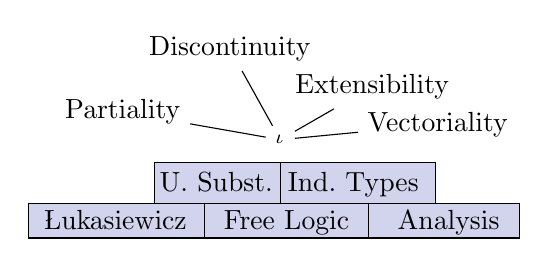
\begin{tikzpicture}[scale=1.6]
    \draw[fill=vblue!20,draw] (0,0) rectangle (1.4,0.275);
    \draw (0.75,0.125) node  {{\L}ukasiewicz\phantom{y}};
    \draw[fill=vblue!20,draw] (1.4,0) rectangle (2.7,0.275) ;
    \draw (2.05,0.125) node {Free Logic};
    \draw[fill=vblue!20,draw] (2.7,0) rectangle (3.9,0.275);
    \draw (3.3,0.125) node {$\reals$ Analysis};
    \draw[fill=vblue!20,draw] (1,0.275) rectangle (2,0.6);
    \draw (1.55,0.425) node {U.\ Subst.\phantom{y}};
    \draw[fill=vblue!20,draw] (2,0.275) rectangle (3.23,0.6);
    \draw (2.58,0.425) node {Ind.\ Types};
    \draw (2,0.78) node (dle){$\dLi$};
    \draw (0.75,1) node (part) {Partiality};
    \draw (1.60,1.5) node (disc) {Discontinuity};
    \draw (2.73,1.2) node (ext) {Extensibility};
    \draw (3.25,0.9) node (vect) {Vectoriality};
    \draw (dle) -- (part);
    \draw (dle) -- (disc);
    \draw (dle) -- (ext);
    \draw (dle) -- (vect);
\end{tikzpicture}
\caption{\dLi features and technical challenges}
\label{fig:dli-overview}
\end{figure}

In the context of the thesis, this section shows that the extended term language used in practice is amenable to a foundational treatment like those provided by theory.
This section also qualifies the author for the remaining foundational tasks: whereas \rref{sec:isabelle-fml} focused on a detailed reproduction of an existing proof calculus, 
\dLi required a wholesale revision of \dL semantics, just as extending \dGL to \CdGL will.
The theoretical developments for \dLi culminate in soundness and equi-expressiveness proofs with respect to \dL, which very much the same kind of results we aim to achieve for the \CdGL theory.

\subsection{Related Work}
As shown in \rref{fig:prover-formalizations}, there are formalizations of \KeYmaeraX~\cite{DBLP:conf/pldi/BohrerTMMP18}, Coq~\cite{DBLP:journals/jfrea/Barras10}, NuPRL~\cite{DBLP:conf/itp/AnandR14}, and HOL4~\cite{DBLP:journals/jar/KumarAMO16}, connecting each to its logical foundation.
With the possible exception of HOL4, each formalization omits features which are theoretically challenging for their specific logic: discontinuous and partial terms in \KeYmaeraX, termination-checking in Coq, or context management in NuPRL.
Thus only a subset of the implementation is guaranteed sound.
When formalizations of theorem provers \emph{do} succeed in reflecting the implementation~\cite{DBLP:journals/jar/KumarAMO16}, they owe a credit to the generality of the underlying theory: it is much more feasible to formalize a general base theory than to formalize ad-hoc extensions as they arise.
Our calculus, as with modern implementations~\cite{DBLP:conf/cade/FultonMQVP15} and machine-checked correctness proofs~\cite{DBLP:conf/cpp/BohrerRVVP17} for \dL, is based on uniform substitution~\cite[\S35,\S40]{Church:1956}: symbols ranging over predicates, programs, etc. are explicitly represented in the syntax.
This improves the ease with which \dLi can be implemented and its soundness proof checked mechanically in future work.
We show that in contrast to \dL, \dLi can directly represent a hybrid system featuring such ODEs, which we base on Hubbard's leaky bucket~\cite[\S4.2]{Hubbard}.
Then the water drains out the cooler at a rate proportional to the square root of the current volume  by Torricelli's Law~\cite{driver1998torricelli}, or rate 0 if the valve is closed.
In contrast to the indexed variables of \QdL~\cite{DBLP:journals/lmcs/Platzer12b}, they are equipped with an induction operator, making it easier to write sophisticated computations.
%
\newcommand{\circsize}{0.3in}
  \begin{figure}
    \centering
    \begin{tikzpicture}[scale=1.6]
    \draw (0,2) node {Prover};
    \draw (1,2) node[rectangle,fill=vblue!20,draw] (nuprl) {NuPRL};
    \draw (2,2) node[rectangle,fill=vblue!20,draw] (coq) {Coq};
    \draw (3.3,2) node[rectangle,fill=vblue!20,draw] (kyx) {\KeYmaeraX};
    \draw (4.6,2) node[rectangle,fill=vblue!20,draw] (hol4) {HOL4};
    \draw (0,1) node {Challenge};
    \draw (0,0) node {Foundation};
    \draw (1,0) node[circle,fill=vblue!20,draw,text width=\circsize] (nuprl-log) {PRL};
    \draw (2,0) node[circle,fill=vblue!20,draw,text width=\circsize] (coq-log) {CIC};
    \draw (3.3,0) node[circle,fill=vblue!20,draw,text width=\circsize] (kyx-log) {\dL};
    \draw (4.6,0) node[circle,fill=vblue!20,draw,text width=\circsize] (hol4-log) {HOL};
    \draw [style=dashed,line width=0.6mm] (nuprl) -- (nuprl-log) node[midway,right=0.025in]  {$\Gamma$};
    \draw [style=dashed,line width=0.6mm] (coq) -- (coq-log) node[midway,right=0.025in]  {$\Downarrow$};
    \draw [style=dashed,line width=0.6mm] (kyx) -- (kyx-log) node[midway,right=0.025in]  {$\rightharpoonup, C^\infty$};
    \draw [-,line width=0.6mm] (hol4) -- (hol4-log) node[midway,above=0.025in,sloped]  {\citeyear{DBLP:journals/jar/KumarAMO16}};
    \end{tikzpicture}
\caption{Prover formalizations and challenges}
\label{fig:prover-formalizations}
  \end{figure}

\chapter{Completed Work:  End-to-End Robot Verification}
%ch:logical-foundations
\label{ch:end-to-end-v}
This chapter describes  works by the author and collaborators which introduce a general approach that enables end-to-end verification while maintaining solid logical foundations and then apply the approach in a case study on the verification of free driving for 2D Dubins-like ground robots.
These works already constitute a major component of the goals of the thesis: what remains in the proposed work is to extend this beyond only verification and monitor synthesis to include controller synthesis while maintaining rigorous foundations.
We begin by motivating end-to-end verification and defining it, then give our approach and case study results in greater detail.

\section{\VeriPhy Pipeline for End-to-End Verification}
\label{sec:veriphy}
Recall our notion of end-to-end verification from \rref{ch:introduction}: we wish to produce formal guarantees that apply to practical implementations of a CPS by proving that the implementation refines a provably safe hybrid system model.
We wish for the refinement process to be fully automatic for the sake of the Engineer who builds the CPS and does not want to do formal proofs.
Granted, the Engineer will need the Logic-User's help to verify the hybrid system model, but this is done only once: it is more important that we need not redo manual proofs each time the Engineer changes their code.
At the same time, each refinement step should provide machine-checkable evidence, in order to satisfy the Logician that the proof is correct.
Our approach, which we will refer to as the \VeriPhy approach (as it is implemented in our tool \VeriPhy), achieves all of the above, as we will now describe.

In light of the fact that a real Engineer might use languages where formal verification is difficult, and that their code may change hundreds of times per day, the \VeriPhy approach employs runtime monitoring so that the Engineer's controller is untrusted.
Specifically, we monitor whether the implementation complies to the source-model.
The Logic-User wants source-model verification to be as simple as possible and the Logician wants safety of the model to closely match an intuitive notion of real-world safety.
For these reasons, the source-model is a hybrid program, verified in \KeYmaeraX with \dL.

\begin{figure*}[tb]
\centering
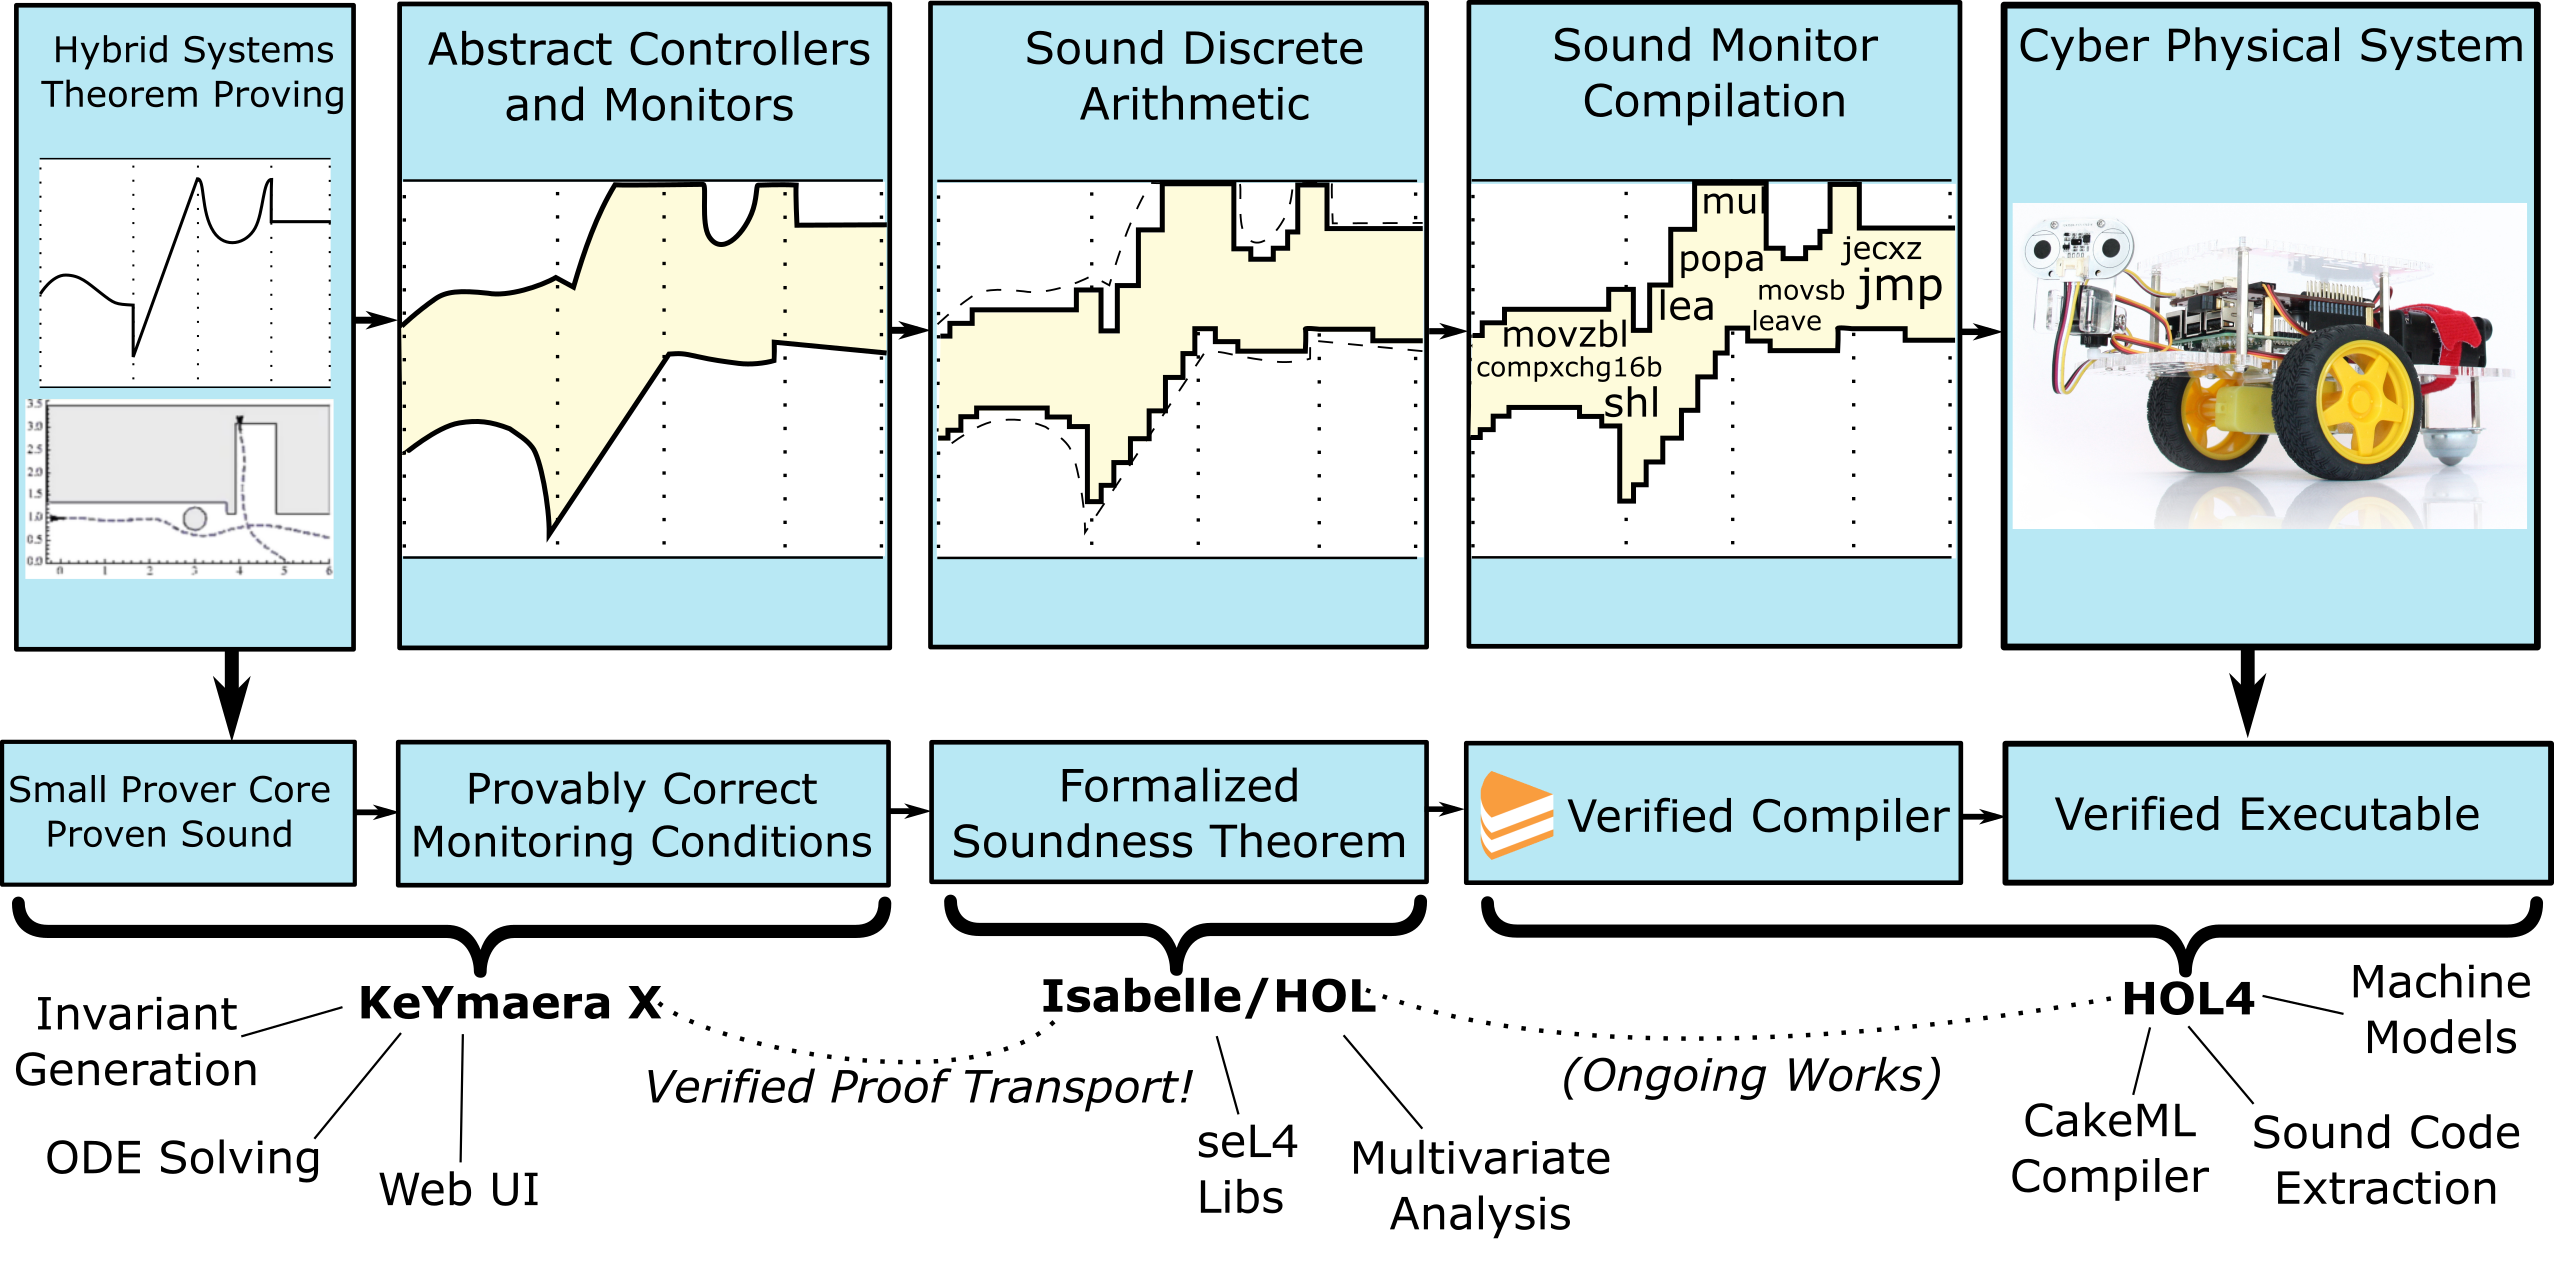
\includegraphics[width=6in]{graphics/veriphy-overview.png}
%\resizebox{6in}{!}{
%\begin{tikzpicture}[->,>=stealth',shorten >=1pt,auto,node distance=2.0cm,
%  thick,
%  model node/.style={rectangle,rounded corners,text centered,fill=black!20,draw,font=\sffamily,inner xsep=0pt,text width=2.7cm},
%  container/.style={rectangle,text centered,draw,fill=gray!10,font=\sffamily,dashed}
%  ]
%  \tikzstyle{stepbox}=[minimum height=3.3\baselineskip]
%  \tikzstyle{outbox}=[]
%  \tikzstyle{optbox}=[dashed]
%\node[model node,stepbox,text width=2.7cm] (model) at (0,0) {CPS Model (\dL)\\$\phi \limply\dibox{\prepeat{\alpha}}\psi$};
%&\node[model node,outbox,text width=2.5cm,below=1.8cm of model] (safetyproof) {System safe\strut};
%\node[model node,stepbox,right=1.1cm of model] (ivmonitor) {Sandbox (\dL)\\ $\phi \limply \dbox{\sandbox}\psi$};
%\node[model node,outbox,below=1.8cm of ivmonitor] (ivmonitorproof) {Sandbox safe\strut};
%\node[model node,outbox,right=1.3cm of ivmonitorproof,yshift=0.1cm] (ptproof) {Intervals, checker sound};
%\coordinate[above=2.2cm of ptproof] (ptanchor);
%\node[model node,outbox,right=0.8cm of ptproof] (cakeproof) {Compilation sound\strut};
%\node[model node,stepbox,above=1.5cm of cakeproof] (cake) {Sandbox\\ (ARM/x64 exec.)};
%
%%step numbers and names
%\node[above=0cm of model,align=center] {Step 1\\\strut Prove model safety};
%\node[above=0cm of ivmonitor,align=center] (step3text) {Step 2\\\strut Synthesize safe sandbox};
%\node[above=0cm of cake,align=center] {Step 3\\\strut Compile};
%
%\draw[-,black,very thick,dashed] (ptproof) -- node[anchor=east,align=center,pos=0.34] {Soundness proof\\PLDI \citeyear[\S2]{DBLP:conf/pldi/BohrerTMMP18}} (ptanchor);
%\draw (model) -- node[anchor=east,align=center] {Safety proof\strut\\PLDI \citeyear[\S3]{DBLP:conf/pldi/BohrerTMMP18}} (safetyproof);
%\draw (model) -- node (myxtactic) {} (ivmonitor);
%\draw (ivmonitor) -- node (ivtactic) {} (cake);
%\draw (ivmonitor) -- node[anchor=east,align=center] {Safety proof\strut\\PLDI \citeyear[\S4]{DBLP:conf/pldi/BohrerTMMP18}} (ivmonitorproof);
%\draw (ivmonitor) -- node (isartactic) {} (cake);
%\draw (ivmonitor) -- (cake) node[pos=0.2] (mid45) {};
%\draw (cake) -- node[anchor=west,align=center] {Soundness proof\\PLDI \citeyear[\S5]{DBLP:conf/pldi/BohrerTMMP18}} (cakeproof);
%
%
%\draw[decoration={brace,amplitude=1em},decorate,black,-]
%    let \p1=($(safetyproof.south west)-(0,1ex)$), \p2=($(ivmonitorproof.south east)-(0,1ex)$) in
%    ({\x2}, {\y2}) -- node[below=2ex] {\KeYmaeraX} ({\x1}, {\y1});
%
%\draw[decoration={brace,amplitude=1em},decorate,black,-]
%    let \p1=($(ptproof.south west)-(0,1ex)$), \p2=($(ptproof.south east)-(0,1ex)$) in
%    ({\x2}, {\y2}) -- node[below=2ex] {\Isabelle} ({\x1}, {\y1});
%
%\draw[decoration={brace,amplitude=1em},decorate,black,-]
%    let \p1=($(cakeproof.south west)-(0,1ex)$), \p2=($(cakeproof.south east)-(0,1ex)$) in
%    ({\x2}, {\y2}) -- node[below=2ex] {HOL4+CakeML} ({\x1}, {\y1});
%\end{tikzpicture}}
%\vspace{-0.06in}
\caption{High assurance artifacts and steps in the \VeriPhy verification pipeline}
\label{fig:pipelineoverview}
\end{figure*}
\begin{itemize}
\item The \ModelPlex tool is invoked to synthesize a \emph{control monitor formula} and \emph{plant monitor formula}, which determine whether control decisions and physical evolutions respectively satisfy the assumptions made of them by the model
\item The monitors are combined with a proven-safe \emph{fallback controller} (which is provided in the input model) to form a \emph{sandbox controller}.
   The sandbox controller applies control decisions provided from an external source (henceforth called the \emph{external controller}) whenever those decisions satisfy the controller monitor,
   and otherwise invokes the fallback controller
\item The sandbox controller is automatically proven safe in \KeYmaeraX, in part by reusing the contents of the hybrid system safety proof
\item The sandbox safety proof is optionally rechecked in the verified proof checker (\rref{sec:isabelle-fml}) to eliminate the \KeYmaeraX core from the trusted base
\item The exact real arithmetic of hybrid systems is replaced with conservative fixed-point interval arithmetic, which is formally proven in Isabelle to be sound
\item The resulting program is proven equivalent to a CakeML program (in HOL4)
\item The equivalent CakeML program is compiled to machine code in a verified compiler
\item The machine code is linked against the users' implementation of sensors and actuators
\end{itemize}
Each step is provably a refinement (\rref{fig:proofchainoverview}) of the step before it, culminating that any execution of the machine-code running on the actual CPS is corresponds to some execution of the source hybrid system.
Because all executions of the source hybrid system were proven safe already, then the execution of the actual CPS is also known to be safe.

Notably, the sensors and actuator drivers, which are provided by the users of \VeriPhy, are trusted.
We justify this by noting that verification of sensing and actuation is a moving target: their hardware changes frequently, and their verification would require rewriting models and their proofs every time that hardware changes.
Because models of hardware still require assumptions on the physical behavior of the hardware's components, even this would not eliminate the trusted hardware base.
For these reasons, \VeriPhy prioritizes providing a simple and well-specified interface for sensing and actuation, which leaves open the possibility of verifying these components in future work.
This interface consists of a handful of CakeML foreign-functions, which have precise specifications in HOL4.
\newcommand{\goback}{\!\!}
\begin{figure}[htb]
\vspace{-0.15in}
\begin{align*}
\iget[state]{\It} & \models \psi \\
& \Uparrow && \goback\text{\small{by \cite[Thm.\ 4]{DBLP:conf/pldi/BohrerTMMP18}}}\\
(\iget[state]{\I},\iget[state]{\It}) &\in \underbracket{\iaccess[\sandbox]{\I}}_{\text{\dL (\KeYmaeraX)}} && \goback\text{\parbox{4cm}{\small{Real arithmetic,\\ nondeterministic}}} \\[-2ex]
& \Uparrow && \goback\text{\small{by \cite[Thm.\ 8]{DBLP:conf/pldi/BohrerTMMP18}}} \\
\bigl(\iget[state]{\I}_I,\iget[state]{\It}_I\bigr) &\in \underbracket{\wsem{\sandbox}{}}_{\text{\dL (Isabelle/HOL)}} && \goback\text{\parbox{4cm}{\small{Interval word arithmetic,\\ nondeterministic}}} \\[-2ex]
& \Uparrow && \goback\text{\small{by \cite[Thm.\ 10]{DBLP:conf/pldi/BohrerTMMP18}}}\\
\bigl(\cmlsem{\iget[state]{\I}}{},\cmlsem{\iget[state]{\It}}{}\bigr) &\in \underbracket{\cmlsem{\cmldet{\sandbox}}{}}_{\text{CakeML (HOL4)}} && \goback\text{\small{\parbox{4cm}{Interval word arithmetic,\\ deterministic}}} \\[-2ex]
& \Uparrow && \goback\text{\small{by CakeML compiler~\cite{DBLP:conf/icfp/TanMKFON16}}}\\
\bigl(\machsem{\iget[state]{\I}}{},\machsem{\iget[state]{\It}}{}\bigr) &\in \underbracket{\machsem{\cmlcompile{\cmldet{\sandbox}}}{}}_{\text{ARM/x64}} && \goback\text{\parbox{4cm}{\small{Interval word arithmetic,\\ machine-executable}}}
\vspace{-0.15in}
\end{align*}
\caption{End-to-end proof chain for end-to-end result}
\label{fig:proofchainoverview}
\end{figure}
\rref{fig:proofchainoverview} shows the chain of formal safety properties proven for the artifacts given in \rref{fig:pipelineoverview}.
One major challenge is that our notion of end-to-end verification demands crossing multiple levels of abstraction, from hybrid systems down to discrete arithmetic and finally machine-code.
For this reason, we incorporated several provers: \KeYmaeraX is used for the source-model proof, Isabelle/HOL is used for the translation into discrete arithmetic, and HOL4 with its verified CakeML compiler is used for final compilation to machine-code.
If we wish to verify sensing and actuation in the future, this could be done by proving in HOL4 that the hardware drivers implement their specifications.

\subsection{Related Work}
\paragraph{Verified Compilation.}
We use the CakeML~\cite{DBLP:conf/icfp/TanMKFON16} verified ML compiler and its associated verification tools~\cite{DBLP:conf/icfp/MyreenO12,DBLP:conf/esop/GueneauMKN17}.
Recent work~\cite{DBLP:conf/esop/HupelN18} also provides extraction of CakeML code from \Isabelle proofs, but its present iteration does not support all features needed in this work.
CakeML is higher-level than other languages such as Clight with verified compilers such as floating-point CompCert~\cite{DBLP:conf/arith/BoldoJLM13}.
This makes the verification of sandbox implementation in CakeML against hybrid systems semantics painless.
We chose this over, e.g., translation validation with unverified compilers~\cite{DBLP:conf/pldi/SewellMK13} since translation validation can be brittle.

Lustre~\cite{DBLP:journals/tse/HalbwachsLR92} is a CPS-centric language with a verified compiler, V\'{e}lus~\cite{DBLP:conf/pldi/BourkeBDLPR17}.
Writing and compiling a Lustre controller provides no end-to-end guarantees because physical modeling and verification are left unanswered.
It could be used as a code generation target, but this would be a detour because the Lustre language differs greatly from hybrid programs.

\paragraph{Machine Arithmetic Verification.}
Machine arithmetic correctness is a major \VeriPhy component.
We verify arithmetic soundness foundationally.
This is an active research area with libraries available in HOL Light~\cite{DBLP:conf/sfm/Harrison06}, Coq~\cite{DBLP:conf/arith/BoldoM10,DBLP:conf/tphol/DaumasRT01,DBLP:conf/mkm/BoldoFM09,DBLP:journals/iandc/Melquiond12}, \Isabelle~\cite{DBLP:journals/afp/Yu13}, etc.
Standalone arithmetic checkers~\cite{DBLP:conf/tacas/2018-1} have also been verified in HOL and Coq~\cite{DBLP:conf/fmcad/BeckerZMDMF18}.
Of these, only PFF in Coq~\cite{DBLP:conf/tphol/DaumasRT01} provides the qualitative rounding correctness results we need, so we prove them in \Isabelle using the seL4~\cite{DBLP:journals/cacm/KleinAEHCDEEKNSTW10} machine word library.
We chose \Isabelle and HOL4 over Coq because their combination of cutting-edge analysis libraries~\cite{DBLP:conf/itp/ImmlerT16}, mature formalization of $\dL$~\cite{DBLP:conf/cpp/BohrerRVVP17}, proof-producing code extraction~\cite{DBLP:conf/icfp/MyreenO12}, and classical foundations positions them well for our end-to-end pipeline.
Static analysis of arithmetic for hybrid systems has been studied~\cite{DBLP:conf/emsoft/MartinezMST10,DBLP:conf/emsoft/MajumdarSZ12,DBLP:conf/cav/BouissouGPTV09}, but without foundational safety proofs for general dynamics.

\section{Case Study: End-to-End Ground Robotics Verification}
\label{sec:ground-robotics}
To validate our claim that \VeriPhy enables end-to-end verification for \dL, it is crucial that we actual implement realistic, verified systems using \VeriPhy.
In doing so, we demonstrate that the \dL models involved can be verified by a real Logic-User and that the software involved can be developed by a real Engineer.
However, the initial research thrust only verified a simple 1D velocity-controlled car~(\rref{ex:driving-game}) and ran it on hardware.
In this section, we develop a 2D acceleration-controlled (Dubins) waypoint-following car with speed limits.
This is far more representative of realistic driving scenarios which require steering and speed enforcement.
It is also far more representative of realistic proofs, as it uses more advanced techniques than those required by the first example, and has more thoroughly stress-tested our tooling.

Our case study includes \dL models, proofs, a simulation which employs the sandbox controller generated by \VeriPhy, and test environments for the simulation.

\subsection{Model}
\label{sec:planar-driving-system}
This section introduces our 2D robot model in \dL.
The Dubins dynamics are bloated by a tolerance, which accounts for imperfect actuation and for discrepancies between the Dubins dynamics and real dynamics of the implementation.
That is, because realistic robots never follow a path perfectly, we will bloat each arc to an annulus section which is more easily followed.
Each waypoint is specified by coordinates $(\xgvar,\ygvar)$, a curvature $\kvar$, and a speed limit $[\vlvar,\vhvar]$ for the robot's velocity $\vvar$ which is to be met by the time the waypoint is reached.
The curvature parameter yields circular arcs (when $\kvar \not= 0$) and lines (when $\kvar=0$) as primitives.

Our hybrid program $\alpha$ is a time-triggered \emph{control-plant} loop: $\alpha\equiv(\ctrl;\plant)^*$.
We use \emph{relative} coordinates: the robot's position is always the origin, from which perspective the waypoint ``moves toward'' the vehicle.
This simplifies proofs (fewer variables) and implementation (real sensors and actuators are vehicle-centric).
The $\plant$ is an ODE describing the robot kinematics:
\begin{align*}
\plant\equiv \{&\D{\xgvar}=-\vvar~\kvar~\ygvar,~\D{\ygvar}=\vvar~(\kvar~\xgvar-1),~\D{\vvar}=\avar,~\D{\tvar}=1 \\
 &\&~\tvar\leq \Tvar ~\land~ \vvar \geq 0\} %  ~\land~ yg > 0
\end{align*}
Here, $\avar$ is an input from the controller describing the acceleration with which the robot is to follow the arc of curvature $\kvar$ to waypoint $(\xgvar,\ygvar)$.
In the equations for $\D{\xgvar},\D{\ygvar}$: \begin{inparaenum}[\it i)]\item The $\vvar$ factor models $(\xgvar,\ygvar)$ moving at linear velocity $\vvar$, \item The $\kvar,\xgvar,\ygvar$\ factors model circular motion with curvature $\kvar$, with $\kvar > 0$ corresponding to counter-clockwise rotation of the waypoint, $\kvar < 0$ to clockwise rotation, and $\kvar = 0$ to straight-line motion, \item The additional $-1$ term in the $\D{\ygvar}$ equation shifts the center of rotation to $\left(\frac{1}{\kvar},0\right)$.
\end{inparaenum}
The equations $\D{\vvar}=\avar$ and $\D{\tvar}=1$ make acceleration the derivative of velocity and $\tvar$ stand for current time.
The domain constraint $\tvar \leq \Tvar \land \vvar \geq 0$ says that the duration of one control cycle shall never exceed a timestep parameter $\Tvar > 0$ representing the maximum delay between control cycles and that the robot never drives in reverse.

The controller's task is to compute an acceleration $\avar$ which slows down (or speeds up) soon enough that the speed limit $\vvar \in [\vlvar,\vhvar]$ is ensured \emph{by the time} the robot reaches the goal.
The controller is written:
\newcommand{\admiss}{\textsf{Go}} % (\xgvar,\ygvar,\vlvar,\vhvar,\kvar,\avar)
\newcommand{\planreq}{\textsf{Feas}} % (\xgvar,\ygvar,\vlvar,\vhvar,\kvar,\avar)
\newcommand{\veps}{\varepsilon}
\newcommand{\annul}{\textsf{Ann}\xspace}
\newcommand{\adjustSpeedDist}{\delta_\mathsf{Lim}\xspace}
\newcommand{\controllableGoalDist}{\mathsf{Lim}}
% %\annul &\equiv
% %\left|\frac{ v~\xgivar~\left(\xgvar^2 +\ygvar^2\right)}{\xgivar^2+\ygivar^2} - v~\xgvar\right| \leq  \veps^2 \tag{a}\\
% %\land&~\ygvar>0 \tag{b} \\
% %\land&~\frac{2~\xgivar~(\xgvar~\ygivar-\xgivar~\ygvar)}{\xgivar^2+\ygivar^2}+\ygvar \leq \ygivar \tag{c}
% %\land&~\ygvar>0 \tag{c}
{\small\begin{align*}
\annul &~\mequiv~\abs{\kvar}\veps \leq 1 \land \Big|\frac{ \kvar~\left(\xgvar^2 +\ygvar^2 - \veps^2 \right)}{2} - \xgvar\Big| < \veps\\
%ygvar>0 included for consistency with the proof (it is also monitored to satisfy our liveness assumption)
\label{eq:planReq} \planreq &~\equiv \annul \land \ygvar{>}0 \land 0{\leq}\vlvar{<}\vhvar \land \Avar\Tvar{\leq}\vhvar-\vlvar \land \Bvar\Tvar{\leq}\vhvar-\vlvar\\
\ctrl &~\equiv~ \prandom{(\xgvar,\ygvar)};\,\prandom{[\vlvar,\vhvar]};\,\prandom{\kvar};\,\ptest{\planreq};\,\underbrace{\prandom{\avar};\,\ptest{\admiss}}_{\ctrlliv}\\
      ~&\hspace*{-5pt}\admiss \equiv-\Bvar\leq \avar \leq\Avar \land \vvar + \avar\Tvar \geq 0 \\
\land & \Bigl(\vvar \leq \vhvar \land \vvar+\avar\Tvar\leq \vhvar ~\lor \\
      & (1+\abs{\kvar}\veps)^2 \Bigl(\vvar\Tvar+\frac{\avar}{2}\Tvar^2 + \frac{(\vvar{+}\avar\Tvar)^2-\vhvar^2}{2\Bvar}\Bigr) + \veps{\leq}\lnorm{(\xgvar,\ygvar)} \Bigr)\\
\land & \Bigl(\vlvar \leq \vvar \land \vlvar \leq \vvar+\avar\Tvar ~\lor\\
      & (1+\abs{\kvar}\veps)^2 \Bigl(\vvar\Tvar+\frac{\avar}{2}\Tvar^2 + \frac{\vlvar^2 - (\vvar{+}\avar\Tvar)^2}{2\Avar}\Bigr) + \veps{\leq}\lnorm{(\xgvar,\ygvar)}\Bigr)\end{align*}}
\noindent where the plan assignment $\prandom{(\xgvar,\ygvar)}$ chooses the next 2D waypoint, the assignment $\prandom{[\vlvar,\vhvar]}$ chooses the speed limit interval, and $\prandom{\kvar}$ chooses any curvature.
The \emph{feasibility} test $\ptest{\planreq}$ determines whether or not the chosen waypoint, speed limit, and curvature are \emph{physically} attainable in the current state under the $\plant$ dynamics (e.g., it checks that there is enough remaining distance to get within the speed limit interval).
We also simplify plans so all waypoints satisfy $\ygvar > 0,$ by subdividing any violating paths automatically.
This simplifies the feedback controller and proofs.
The abbreviation $\ctrlliv$ names just the control code responsible for deciding \emph{how} the waypoint is followed rather than \emph{which} waypoint is followed.


In $\planreq,$ formula $\annul$ says we are within the \emph{annulus section} (\rref{fig:circlestaging}) ending at the waypoint $(\xgvar, \ygvar)$ with the specified curvature $\kvar$ and width $\epsilon$.
A larger choice of $\veps$ yields more error tolerance in the sensed position and followed curvature at the cost of an enlarged goal region.
Formula $\annul$ also contains a simplifying assumption that the radius of the annulus is at least $\epsilon$.
$\planreq$ also says the speed limits are assumed distinct and large enough to not be crossed in one control cycle.

\begin{figure}[h!]
\centering
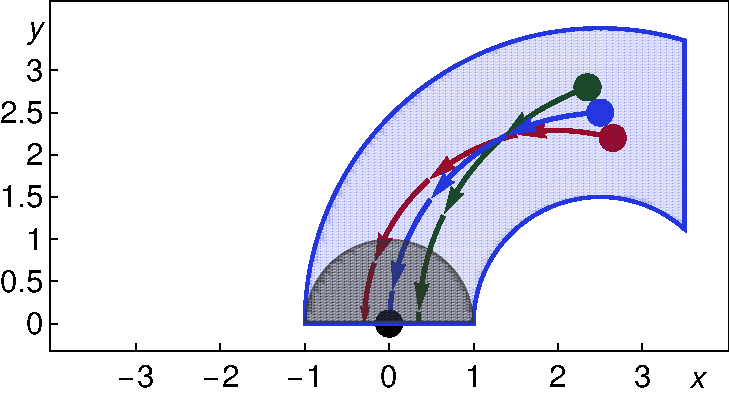
\includegraphics[width=0.3\textwidth]{graphics/fig-ode3.pdf}
\caption{Annular section through the (blue) waypoint $(2.5,2.5)$. Trajectories from the displaced green and red waypoints with slightly different curvatures remain within the annulus.}\label{fig:circlestaging}
\label{fig:circlestaging}
\end{figure}

The \emph{admissibility} test $\ptest{\admiss}$ checks that the chosen $\avar$ will take the robot to its goal with a safe speed limit, by \emph{predicting future motion} of the robot.
We illustrate this with the upper bound conditions.
The bound will be satisfiable after one cycle if either the chosen acceleration $\avar$ already maintains speed limit bounds ($\vvar \leq \vhvar \land \vvar{+}\avar\Tvar \leq \vhvar$) or when there is enough distance left to restore the limits before reaching the goal.
For straight line motion ($\kvar=0$), the required distance can simply be found by integrating acceleration and speed:
\begin{equation*}
\underbrace{\vvar\Tvar+\frac{\avar}{2}\Tvar^2}_{\mathclap{\text{distance in time}~\Tvar}} + \frac{(\overbrace{\vvar{+}\avar\Tvar}^{\mathclap{\text{speed in time}~\Tvar}})^2-\vhvar^2}{2\Bvar} + \veps \leq \lnorm{(\xgvar,\ygvar)}
\end{equation*}
where $\avar \in [-\Bvar,\Avar]$.
The extra factor of $(1 + \abs{k}\veps)^2$ for curved motion accounts for the fact that an arc along the inner side of the annulus is shorter than one along the outside (\rref{fig:circlestaging}).

\subsection{Proofs}
In contrast to prior works~\cite{DBLP:journals/ijrr/MitschGVP17}, this work contains both safety and liveness proofs for the full 2D dynamics.\footnote{In the interest of full disclosure, the modeling and proof sections were largely performed by collaborators in this work. The present author provided simulations, writing, integration with \VeriPhy and advice on the modeling and proof tasks. In contrast, the modeling and proofs in the proposed work are to be performed by the present author}.
In many ways, this lays a foundation for the proposed work because a proof of winnability for a hybrid game will contain both liveness-like (strategy for our player) and safety-like components (strategy for the opponent).
Taken at surface value, the safety theorem says that speed limits are obeyed whenever the robot reaches a waypoint
\begin{theorem}[Safety]
\label{thm:safe}
The following \dL formula is valid:
\begin{align*}
&\Avar{>}0 \land \Bvar{>}0 \land \Tvar{>}0 \land \veps{>}0 \land \linv \limply \\
&\dbox{\prepeat{(\ctrl;\plant)}}{\big(\enorm{(\xgvar,\ygvar)} \leq \veps \limply \vvar \in [\vlvar,\vhvar]\big)}
\end{align*}
\end{theorem}
Taken more broadly, safety also includes the fact that the robot always remains within an $\epsilon$ annulus around the arc leading to the waypoint, which arises as part of the loop invariant used to prove \rref{thm:safe}.
The first four assumptions ($\Avar{>}0 \land \dots \land \veps{>}0$) are basic sign conditions on the symbolic constants used in the model. 
The final assumption, $\linv$, is the loop invariant.
The full definition of $\linv$ is deferred to \rref{sec:ground-robotics}.
We write $\enorm{(\xgvar,\ygvar)}$ for the Euclidean norm $\sqrt{\xgvar^2 + \ygvar^2}$ and consider the robot ``close enough'' to the waypoint when $\enorm{(\xgvar,\ygvar)} \leq \veps$ for our chosen goal size $\veps$.
%The theorem states that no matter which (admissible) control decisions are made, whenever the vehicle is in the goal region of size $\veps$, it obeys the speed limit $\vvar \in [\vlvar,\vhvar]$.
While this captures the desired notion of safety, it does not prove that the robot can actually reach the goal, which is a \emph{liveness} property:
\begin{theorem}[Liveness]
\label{thm:liveness}
The following \dL formula is valid:
\begin{align*}
&\Avar{>}0 \land \Bvar{>}0 \land \Tvar{>}0 \land \veps{>}0 \land \linv \limply \\
&\dbox{\prepeat{(\ctrl;\plant)}}{\Big( \vvar{>}0 \land \yvar{>}0 \limply }\\
&\ \ \ \ \ddiamond{\prepeat{(\ctrlliv;\plant)}}{\big(\enorm{(\xgvar,\ygvar)} \leq \veps~\land~\vvar \in [\vlvar,\vhvar]\big)} \Big)
\end{align*}
%where $\ctrlliv$, as before, controls $\avar$.
\end{theorem}

This theorem has the same assumptions as \rref{thm:safe}. 
It says that no matter how long the robot has been running ($\dbox{\prepeat{(\ctrl;\plant)}}{}$), 
then if some simplifying assumptions still hold ($\vvar{>}0\land\yvar{>}0$) 
the controller can be continually run ($\ddiamond{\prepeat{(\ctrlliv;\plant)}}{}$) with admissible acceleration choices $(\ctrlliv)$ to reach the present goal \((\enorm{(\xgvar,\ygvar)} \leq \veps)\) within the desired speed limits \((\vvar \in [\vlvar,\vhvar])\).
The simplifying assumptions $\vvar{>}0\land\yvar{>}0$ say the robot is still moving forward and the waypoint is still in the upper half-plane, i.e., we have not run \emph{past} the waypoint.

The liveness theorem is invaluable because it validates the \dL model: if it were not even possible at the level of the \dL model to achieve liveness, then it would be absolutely impossible at the level of implementation to achieve liveness.
Because it is undesirable to change the model drastically once implementation has started (i.e., delays in modeling and verification will trickle down to greater delays in implementation and testing), it is valuable to have this confidence in the model before implementation even begins.
Moreover, the combination of safety and liveness gives us confidence that a game generalization of this proof will succeed, as the main components of a game proof are liveness and safety reasoning.

\subsection{Simulations} 
In order to claim that \VeriPhy has been evaluated on a realistic system implementation, it is essential that we choose a simulation platform that is reasonably faithful to the physics of actual autonomous cars.
For this purpose we chose the AirSim~\cite{shah2018airsim} simulator, which is notable for combining top-notch visuals, reasonable physics, and an open-source code base that is particularly friendly to modification.
While some aspects of the underlying physics engine are closed-source, many aspects are open to customization, including for example the details of wheels and suspensions, and the center of gravity.
For this reason and because AirSim has been successfully applied in dozens of projects, we have good reason to believe its physics model is more faithful than any purpose-built one-off simulation would be.

In AirSim, the author implemented several basic control algorithms known as \emph{bang-bang} and \emph{proportional-derivative}.
The author developed several driving environments for testing, shown in \rref{fig:patrol-plan}
%bang-bang and PD (proportional-derivative) controllers in AirSim as well as several environments which provided a variety of driving conditions with turns of different radii.
%The environments and the evaluation results are summarized below:
\begin{figure*}[tb]
\centering
\begin{minipage}[b]{2in}\centering
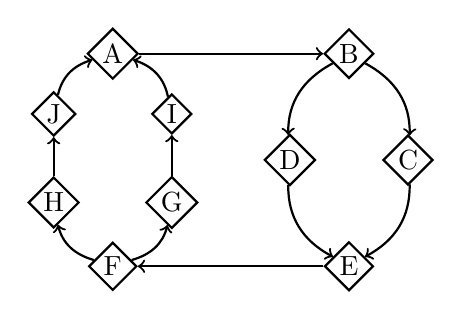
\begin{tikzpicture}[->,draw,thick,yscale=0.9,inner sep=1pt]
\tikzstyle{arc}=[circle,draw]
\tikzstyle{line}=[rectangle,draw]
\tikzstyle{way}=[diamond,draw]
\node[way] (a) at (1,3) {A};
\node[way] (b) at (4,3) {B};
\node[way] (c) at (4.75,1.5) {C};
\node[way] (d) at (3.25,1.5) {D};
\node[way] (e) at (4,0) {E};
\node[way] (f) at (1,0) {F};
\node[way] (g) at (1.75,0.90) {G};
\node[way] (h) at (0.25,0.90) {H};
\node[way] (i) at (1.75,2.15) {I};
\node[way] (j) at (0.25,2.15) {J};
\draw (a) -> (b);
\draw (b) edge [bend left] node {} (c);
\draw (b) edge [bend right] node {} (d);
\draw (c) edge [bend left]node {} (e);
\draw (d) edge [bend right] node {} (e);
\draw (e) -> (f);
\draw (f) edge [bend left]  node {} (h);
\draw (f) edge [bend right] node {} (g);
\draw (h) -> (j);
\draw (g) -> (i);
\draw (j) edge [bend left]  node {} (a);
\draw (i) edge [bend right] node {} (a);
\end{tikzpicture}
\subcaption{Example mission}\label{fig:patrol-mission-plan}\end{minipage}
\begin{minipage}[b]{1.51in}\centering
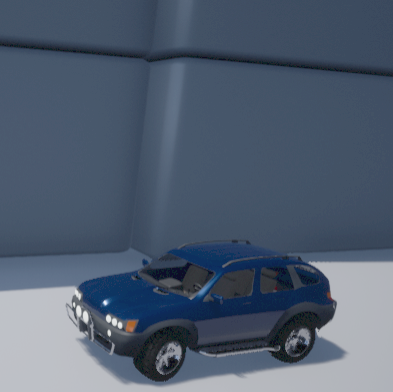
\includegraphics[width=1.51in,clip,trim=0 0 0 50]{graphics/airsim.png}
\subcaption{Simulator}\label{fig:simulator}\end{minipage}
%\begin{minipage}[b]{.3\linewidth}\centering
%\includegraphics[width=1.95in]{graphics/robot.jpg}
%\subcaption{RC car}\label{fig:rccar}
%\end{minipage}
\begin{minipage}[b]{0.15\textwidth}\centering
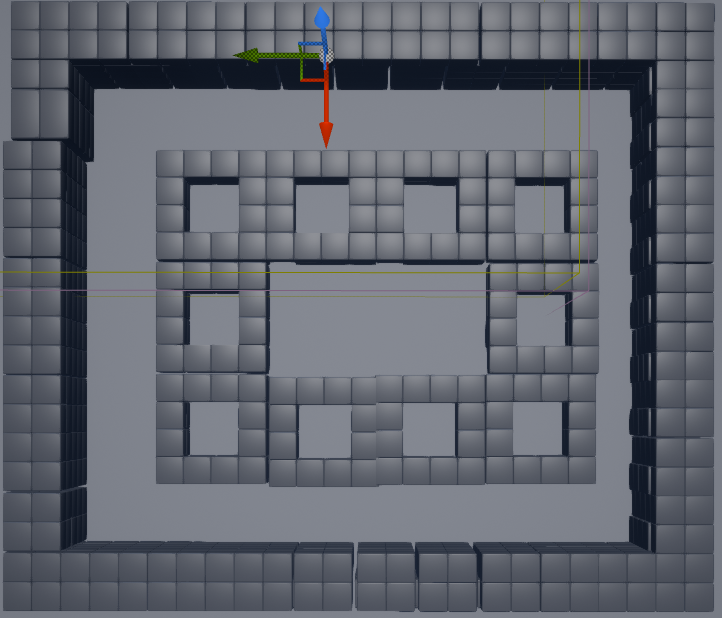
\includegraphics[width=1in]{graphics/screen1.png}
\subcaption{Rectangle}\label{fig:rect}\end{minipage}
\begin{minipage}[b]{0.15\textwidth}\centering
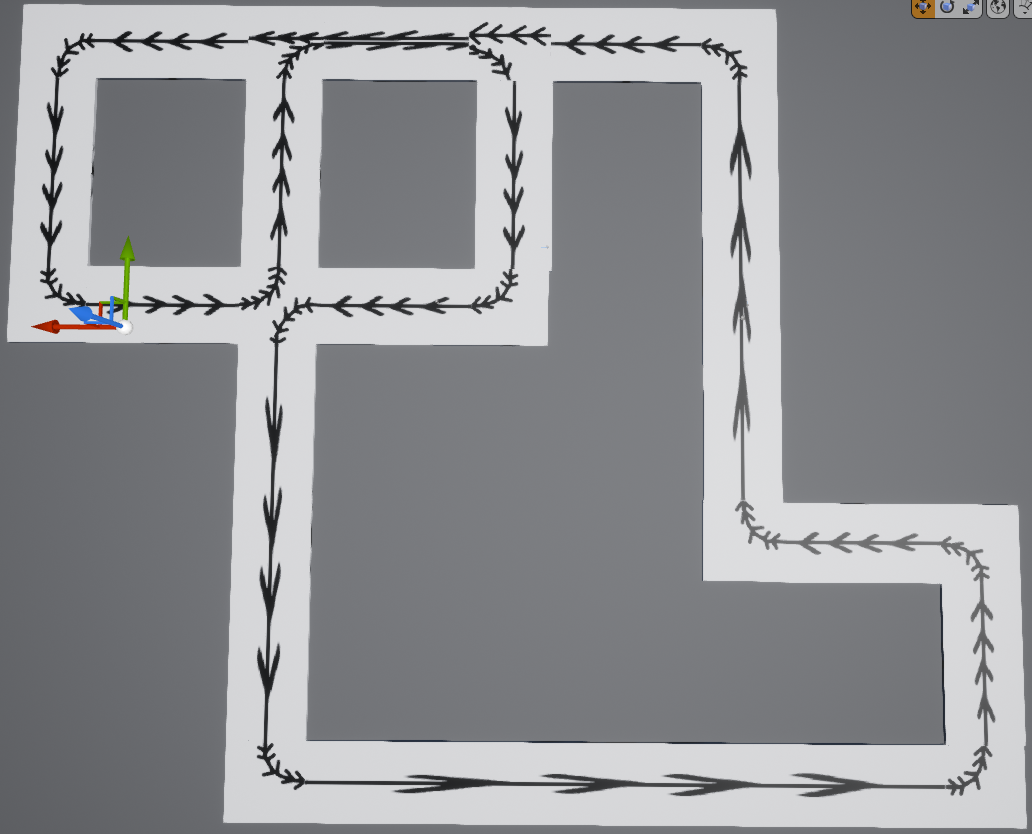
\includegraphics[width=1in]{graphics/screen2.png}
\subcaption{Tight turns}\label{fig:turns}\end{minipage}
\begin{minipage}[b]{0.15\textwidth}\centering
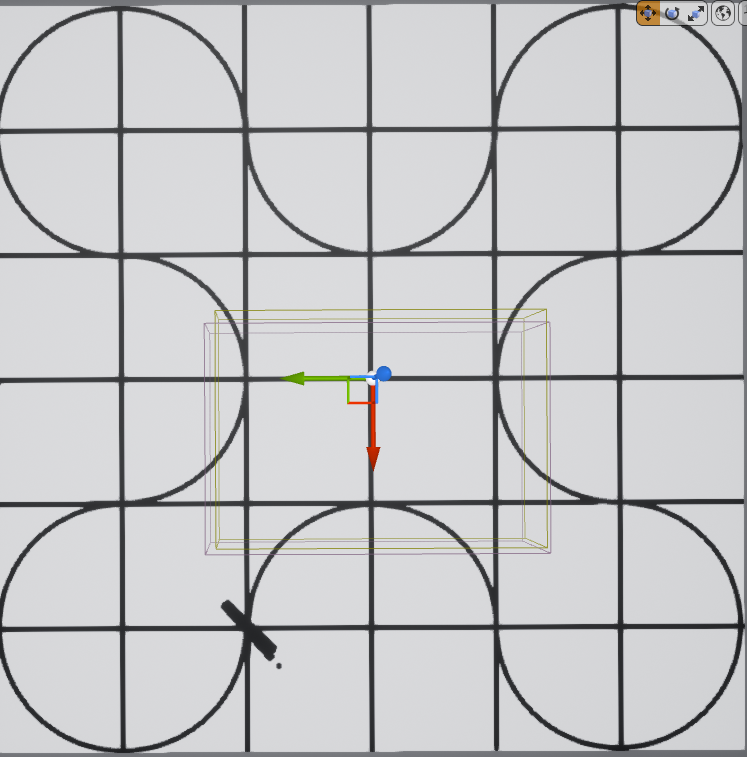
\includegraphics[width=0.8in]{graphics/screen3.png}
\subcaption{Large clover}\label{fig:clover}\end{minipage}
\caption{Implementation and environments built in AirSim}
\label{fig:patrol-plan}
\end{figure*}
The simulations showed that while it is rare to achieve zero errors, failure rates in the single digits are attainable, which suffice to complete all environments.
Moreover, a major challenge we solved was to develop a simulation which worked seamlessly with the monitors, themselves synthesized from the model.
The model and proof were iteratively developed using feedback from the resulting monitors.
Our relatively low failure rates attested that our simple model is yet general enough to describe control decisions and physical dynamics that arise in practice.
Thus our formal link from \dL to CPS execution can be made to work in practice for nontrivial driving scenarios.
%\begin{table*}
%\caption{Average speed, Monitor failure rates, plant violation rates, for AirSim and human driver in Rectangle, Turns, and Clover for Patrol missions}
%\label{tab:results}
%\centering
%\begin{tabular}{l|l|l|l|l|l|l|l|l|l|l|l|l|l|l|l}
%\bottomrule        & \multicolumn{5}{|c|}{Avg.\ Speed (m/s)} & \multicolumn{5}{c|}{Ctrl Fail.} & \multicolumn{5}{c|}{Plant Fail.} \\
%World   & BB   & \textbf{PD1}   & PD2   & PD3     & Human     & BB     & \textbf{PD1}      & PD2    & PD3    & Human  & BB    & \textbf{PD1} & PD2   & PD3 & Human \\\toprule
%Rect    & 9.2  & \textbf{6.24}   & 8.47 &  13.5   & 12.6      & 1.4\%  & \textbf{0\%}      & 0\%    & 0.17\% & 3.0\%  & 9.8\% & \textbf{1.8\%} & 1.2\%  & 4.0\%   & 10.5\%  \\
%Turns   & 8.3  & \textbf{4.54}   & 5.93 &  10.4   & 10.8      & 3.0\%  & \textbf{0\%}      & 3.3\%  & 0.75\% & 3.5\%  & 11\%  & \textbf{0.2\%} & 0.4\%  & 3.1\%   & 5.63\%  \\
%Clover  & 13.8 & \textbf{13.9}   & 18.2 &  29.8   & 29.3      & 6.6\%  & \textbf{0.3\%}    & 0\%    & 0.32\% & 0.66\% & 28\%  & \textbf{1.7\%} & 44\%   & 38.1\%  & 24.4\%
%\end{tabular}
%\end{table*}
%\rref{tab:results} gives the results of several controllers (PD1 is the slowest PD controller, PD3 the fastest) as well as a human pilot (the author) on all environments.
%Overall, the slow PD controller had the best monitor failure rates of any controller.
%Qualitatively, the results tell us that while perfect failure 0\% rates are not always attainable, low failure rates are achievable in practice, where low control failure rates mean that the fallback controller will rarely need to engage and low plant failure rates mean that because physical assumptions are rarely violated, the formal guarantees provided by \VeriPhy are applicable almost all the time.


\subsection{Related Work}
Related work in formal methods and robotics has applied synthesis and verification to safe control of robotic systems.
The present work is unique among these in its use of a verified-safe sandbox controller to enforce compliance between the implementation and formal model for a realistic robot simulation with an expressive correctness guarantee.

\subsubsection{Simulation}
Simulation is an essential part of evaluating models and designs for any robotic system.
Multiple simulation platforms are available, of which AirSim~\cite{shah2018airsim} is a recent platform for UAVs and autonomous cars.
Other simulators would likely have worked as well, but we chose AirSim because it is configured with high-fidelity physical and visual models out of the box, reducing the chances of introducing modeling errors.

\chapter{Completed Work: \CGL: Constructive Game Logic}
\label{ch:cgl}
\newcommand{\projUp}[2]{{#1}\uparrow{#2}}
\newcommand{\projDown}[3]{{#1}\downarrow{#2(#3)}}
\newcommand{\projBV}[3]{\projDown{#1}{#2}{\boundvars{#3}^\complement}}
\newcommand{\sapp}[2]{#1(#2)}
\newcommand{\sadj}[2]{#1^*(#2)}
\newcommand{\spp}[1]{\sapp{\sigma}{#1}}
\newcommand{\adj}[1]{\sadj{\sigma}{#1}}
\newcommand{\drv}{\mathcal{D}}
\newcommand{\nzvar}{\textit{nz}}
%\newcommand{\invvar}{\textit{inv}}	
\newcommand{\convvar}{\textit{cnv}}
\newcommand{\erefl}{\textsf{refl}}
\newcommand{\pstep}{\textsf{step}}
\newcommand{\modvar}{\textit{mod}}
\newcommand{\monvar}{\textsf{m}
}
\newcommand{\rangevar}{\textsf{Range}}
\newcommand{\testvar}{\textsf{test}}
\newcommand{\elem}[2]{\textsf{Dec}[#1](#2)}
\newcommand{\spc}{\hspace{0.15in}}
\newcommand{\kwmod}{\textsf{mod}}
\newcommand{\emod}[2]{#1~\kwmod~#2}
\newcommand{\kwdiv}{\textsf{div}}
\newcommand{\ediv}[2]{#1~\kwdiv~#2}
\newcommand{\kwsig}{\Sigma}
\newcommand{\sig}[1]{\kwsig(#1)}
\newcommand{\nim}{\textsc{Nim}}
\newcommand{\cake}{\textsc{CC}}
\newcommand{\interp}{I}
\newcommand{\valset}[1]{\mathfrak{V}(#1)}
\newcommand{\kwbool}{\m{\mathbb{B}}}
\newcommand{\kwint}{\m{\mathbb{Z}}}
\newcommand{\kwreal}{\m{\mathbb{R}}}
\newcommand{\kwintsig}{\Xi}
\newcommand{\intsig}[1]{\kwintsig(#1)}
\newcommand{\churchkleene}{\omega_{\text{CK}}}
\newcommand{\restL}[1]{#1_L}
\newcommand{\restR}[1]{#1_R}
\newcommand{\apL}[1]{#1_{\langle{0}\rangle}}
\newcommand{\apR}[1]{#1_{\langle{1}\rangle}}
\newcommand{\dpL}[1]{#1_{[0]}}
\newcommand{\dpR}[1]{#1_{[1]}}

\newcommand{\va}{a}
\newcommand{\vb}{b}
\newcommand{\vca}{\overline{a}}
\newcommand{\vcb}{\overline{b}}

\newcommand{\btt}{\texttt{tt}}
\newcommand{\bff}{\texttt{ff}}
\newcommand{\stt}{\top}
\newcommand{\sff}{\bot}
\newcommand{\demonactive}[2]{\textrm{aD}(#1,#2)}
\newcommand{\demondormant}[2]{\textrm{dD}(#1,#2)}
\newcommand{\sren}[3]{\urename[{#1}]{#2}{#3}}%{\subst[{#1}]{#2}{#3}}
\newcommand{\ssub}[3]{\subst[{#1}]{#2}{#3}}
\newcommand{\eren}[3]{\urename[{#1}]{#2}{#3}}%{\subst[{#1}]{#2}{#3}}
\newcommand{\earen}[2]{\urename[{#1}]{\boundvars{#2}}{\vec{y}}}%{\subst[{#1}]{\boundvars{#2}}{\vec{y}}}

\newcommand{\allcon}{\allregion}
\newcommand{\somesemi}[2]{\epsilon #1~|~#2}

\newcommand{\rzF}[2]{#1 \vdash #2}
\newcommand{\rzA}[3]{\langle{#2}\rangle(#1)=(#3)}
\newcommand{\rzD}[3]{[{#2}](#1)=(#3)}
\newcommand{\rzFst}[1]{#1_0}
\newcommand{\rzSnd}[1]{#1_1}
\newcommand{\rzThd}[1]{#1_2}
\newcommand{\rzFrt}[1]{#1_3}
\newcommand{\rzApp}[2]{#1\,#2}
\newcommand{\sa}{\omega}
\renewcommand{\sb}{\nu}
\newcommand{\Sc}{\mu}
\renewcommand{\aa}{a}
\newcommand{\ab}{A}
\newcommand{\ac}{\aleph}
\newcommand{\da}{d}
\newcommand{\db}{D}
\newcommand{\dc}{\delta}
\newcommand{\allRz}{\mathcal{R}\mathbf{z}}
\newcommand{\rzfor}[1]{#1\,\allRz}

\newcommand{\mto}{\rightharpoonup}
\newcommand{\esub}[3]{[{#3}/{#2}]{#1}}
\newcommand{\tsub}[3]{\subst[#1]{#2}{#3}}

%\newcommand{\rzF}[2]{#1 \vdash #2}
%\newcommand{\rzA}[3]{\langle{#2}\rangle(#1)=(#3)}
%\newcommand{\rzD}[3]{[{#2}](#1)=(#3)}
\newcommand{\rzNil}{\epsilon}
\newcommand{\rzCons}[2]{(#1,#2)}
\newcommand{\rzBLam}[2]{\lambda #1:\allstate.~#2}
\newcommand{\rzHOLam}[3]{\Lambda #1:\rzfor{#2}.~#3}
\newcommand{\rzFOLam}[3]{\Lambda #1:#2.~#3}
%\newcommand{\rzApp}[2]{#1\,#2}
\newcommand{\fintR}[1]{\fint{#1}} %{#1#2}
\newcommand*{\strategyforR}[2][]{{#2}\Langle{#1}\Rangle}
\newcommand*{\istrat}[3][]{\strategyforR[#1]{#2}^{#3}}

\newcommand*{\dstrategyforR}[2][]{{#2}\lenvelopewide{#1}\renvelopewide}
%{{#2}\llbracket{#1}\rrbracket}
\newcommand*{\idstrat}[3][]{\dstrategyforR[#1]{#2}^{#3}}
\newcommand{\cint}[1]{\fint{\bigwedge #1}}
\newcommand{\cintR}[1]{\fintR{\bigwedge #1}}
\newcommand{\seq}[2]{#1 \vdash #2}
\newcommand{\proves}[3]{#1\allowbreak\vdash #2 \allowbreak \mathop{:} #3}


\newcommand{\eprojL}[1]{\pi_1{#1}}
\newcommand{\eprojR}[1]{\pi_2{#1}}
\newcommand{\eProjL}[1]{\lstrike\pi_1{#1}\rstrike}
\newcommand{\eProjR}[1]{\lstrike\pi_2{#1}\rstrike}
\newcommand{\edprojL}[1]{\langle\pi_1{#1}\rangle}
\newcommand{\edprojR}[1]{\langle\pi_2{#1}\rangle}
\newcommand{\ebprojL}[1]{[\pi_1{#1}]}
\newcommand{\ebprojR}[1]{[\pi_2{#1}]}

\newcommand{\edOpencons}{\langle}
\newcommand{\edClosecons}{\rangle}
\newcommand{\edSepcons}{,}
\newcommand{\edcons}[2]{\edOpencons{#1}\edSepcons{#2}\edClosecons}
%\newcommand{\edcons}[2]{\langle#1,#2\rangle}
\newcommand{\ebOpencons}{[}
\newcommand{\ebSepcons}{,}
\newcommand{\ebClosecons}{]}
\newcommand{\ebcons}[2]{\ebOpencons#1\ebSepcons#2\ebClosecons}
\newcommand{\eCons}[2]{\lstrike{#1,#2}\rstrike}
\newcommand{\eSnoc}[2]{\llensehat{#1,#2}\rlensehat}
\newcommand{\pmodality}[2]{\llensehat{#1}\rlensehat{#2}}
\newcommand{\econs}[2]{\eCons{#1}{#2}}
\newcommand{\einjL}[1]{\ell \cdot #1}
\newcommand{\einjR}[1]{r \cdot #1}
\newcommand{\kwcase}{\textrm{case}}
\newcommand{\ecaseHead}[1]{\langle\kwcase\textrm{ }#1{\text{\textrm{ of }}}}
\newcommand{\ecaseLeft}[2]{#1\Rightarrow~#2}
\newcommand{\ecaseRight}[2]{~|~#1\Rightarrow~#2}
\newcommand{\ecaseEnd}{\rangle}
\newcommand{\ecasegen}[5]{\ecaseHead{#1}\allowbreak\ecaseLeft{#2}{#3}\allowbreak\ecaseRight{#4}{#5}\ecaseEnd}
\newcommand{\ecase}[3]{\ecasegen{#1}{\ell}{#2}{r}{#3}}
\newcommand{\edcase}[3]{\ecase{#1}{#2}{#3}}
\newcommand{\ercase}[3]{\langle\textrm{case}_*\ #1\text{ of }\pvs\Rightarrow~#2~|~\pvg\Rightarrow#3\rangle}
\newcommand{\eCase}[3]{\lstrike\kwcase\textrm{ }#1\textrm{ of }\allowbreak\ell\Rightarrow~#2~\allowbreak|~r\Rightarrow~#3\rstrike} %\{\textrm{case}\}\ #1\textrm{ of }\ell.~#2~|~r.~#3

\newcommand{\edinjL}[1]{\langle\ell \cdot #1\rangle}
\newcommand{\edinjR}[1]{\langle r \cdot #1\rangle}
\newcommand{\eInjL}[1]{\lstrike\ell \cdot #1\rstrike}
\newcommand{\eInjR}[1]{\lstrike{r \cdot #1}\rstrike}
\newcommand{\kwrep}{\textrm{rep}}
\newcommand{\erep}[3]{{#1}\textrm{ }\kwrep\text{ }#3.~{#2}}
\newcommand{\eapp}[2]{#1\ #2}
\newcommand{\elamgen}[3]{\lambda #1:#2.~ #3}
\newcommand{\eplam}[2]{\elamgen{\pvx}{#1}{#2}}
\newcommand{\etlam}[2]{\elamgen{x}{#1}{#2}}
\newcommand{\ebseq}[1]{[\iota~#1]}
\newcommand{\ebseqinv}[1]{[\iota~{#1}^{-1}]}
\newcommand{\edseq}[1]{\langle\iota~#1\rangle}
\newcommand{\edseqinv}[1]{\langle\iota~{#1}^{-1}\rangle}
\newcommand{\eSeq}[1]{\lstrike\iota~#1\rstrike}
\newcommand{\eSeqinv}[1]{\lstrike\iota~{#1}^{-1}\rstrike}
\newcommand{\ebOpenswap}{[\textrm{yield }}
\newcommand{\ebCloseswap}{]}
\newcommand{\ebswap}[1]{\ebOpenswap#1\ebCloseswap}
\newcommand{\edOpenswap}{\langle\textrm{yield }}
\newcommand{\edCloseswap}{\rangle}
\newcommand{\edswap}[1]{\edOpenswap#1\edCloseswap}
%\llensehat \rlensehat  \lstrike \rstrike
\newcommand{\eSwap}[1]{\lstrike\textrm{yield }#1\rstrike}
\newcommand{\ePaws}[1]{\llensehat\textrm{yield }#1\rlensehat}
\newcommand{\emonInfix}[1]{{\circ_{#1}}}
\newcommand{\emon}[3]{{#1} \emonInfix{#3} {#2}}
%\newcommand{\eQEpos}{\textrm{QE}_{pos}}
%\newcommand{\eQEneg}{\textrm{QE}_{neg}}
\newcommand{\eQE}[2]{\textsf{FO}[#1](#2)}
%\newcommand{\eQEN}[1]{\textsf{QE}[#1]_\mathbb{N}}
%\newcommand{\eQER}[1]{\textsf{QE}[#1]_\mathbb{R}}
\newcommand{\emetsplit}{\textrm{split}\met}
\newcommand{\esplit}[3]{\textrm{split }{[#1\sim#2]}~#3}
\newcommand{\kwstop}{\textrm{stop}}
\newcommand{\kwgo}{\textrm{go}}
\newcommand{\estop}[1]{\langle\kwstop\ #1\rangle}
\newcommand{\ego}[1]{\langle\kwgo\ #1\rangle}
\newcommand{\kwroll}{\textrm{roll}}
\newcommand{\kwunroll}{\textrm{unroll}}
\newcommand{\ebroll}[1]{[\kwroll\ {#1}]}
\newcommand{\ebunroll}[1]{[\kwunroll\ #1]}
\newcommand{\eRoll}[1]{\lstrike\kwroll\ #1\rstrike}
\newcommand{\eUnroll}[1]{\lstrike\kwunroll\ #1\rstrike}
\newcommand{\eghost}[4]{\textrm{Ghost}[#1=#2](#3.~#4)}
\newcommand{\eAsgn}[4]{\lstrike\humod{#2}{\eren{f}{#2}{#1}}\text{ in }#3.~#4\rstrike}
\newcommand{\eAsgneq}[4]{\eAsgn{#1}{#2}{#3}{#4}}
\newcommand{\etconsgen}[5]{\langle{\eren{#4}{#1}{#2}}~{{:}{*}}~#3.~#5\rangle}
\newcommand{\etcons}[2]{\etconsgen{x}{y}{\pvx}{#1}{#2}}
\newcommand{\ietcons}[3]{\langle{\eren{#2}{#1}{~}}~{{:}{*}}~#3\rangle}

\newcommand{\ebasgneq}[4]{[\humod{#2}{\eren{f}{#2}{#1}}\text{ in }#3.~#4]}
\newcommand{\edasgneq}[4]{\langle\humod{#2}{\eren{f}{#2}{#1}}\text{ in }#3.~#4\rangle}
\newcommand{\edasgn}[4]{\edasgneq{#1}{#2}{#3}{#4}}
\newcommand{\ebasgn}[4]{\ebasgneq{#1}{#2}{#3}{#4}}
\newcommand{\iebasgn}[2]{[\humod{#1}{\eren{f}{#1}{~}}\text{ in }~#2]}
\newcommand{\iedasgn}[2]{\langle\humod{#1}{\eren{f}{#1}{~}}\text{ in }~#2\rangle}
%\newcommand{\iedasgn}[2]{\edasgneq{~}{#1}{#1}{#2}}
%\newcommand{\iebasgn}[2]{\ebasgneq{~}{#1}{#1}{#2}}

\newcommand{\eunpack}[2]{\textrm{unpack}(#1,\pvx y.~#2)}
\newcommand{\ewhile}[2]{\textrm{while}(#1 > 0)\{#2\}}
\newcommand{\eloopelim}[3]{(#1, x.~{#2}^{#3})}
\newcommand{\efpgen}[5]{\textit{FP}(#1, #2.~#3, #4.~#5)}
\newcommand{\efp}[3]{\efpgen{#1}{\pvs}{#2}{\pvg}{#3}}
\newcommand{\met}{\ensuremath{\mathcal{M}}}
\newcommand{\conv}{\varphi\xspace}
\newcommand{\Gemp}{\cdot}
\newcommand{\issimp}[1]{{#1}\ \textrm{simp}}
\newcommand{\eforHead}[4]{\textrm{for}(#1:\conv(\met)={#2};#3;{#4})} %#3:\met>0\land\met_0=\met
\newcommand{\eforBody}[1]{\{#1\}}
\newcommand{\eforgen}[5]{\eforHead{#1}{#2}{#3}{#4}\eforBody{#5}}
\newcommand{\efor}[2]{\eforgen{\pvx}{#1}{\pvy}{#2}{\alpha}}
\newcommand{\oldof}[1]{\textrm{old}(#1)}
\newcommand{\isnorm}[1]{#1\textsf{ normal}}
\newcommand{\allpt}{\mathbf{Pt}}
\newcommand{\alltrace}[1]{\mathbf{Tr}(#1)}
\newcommand{\dinline}[2]{\sigma_{\dbox{#1}{}}{(#2)}}
\newcommand{\ainline}[2]{\sigma_{\ddiamond{#1}{}}{(#2)}}
\newcommand{\case}{\textbf{Case}\xspace}
\newcommand{\spost}[2]{\mathsf{sp}(#1,#2)}
\newcommand{\kwassume}{\textbf{assume}}
\newcommand{\kwassert}{\textbf{assert}}
\newcommand{\kwlet}{\textbf{let}}
\newcommand{\kwstate}{\textbf{state}}
\newcommand{\kwsolve}{\textbf{solve}}
\newcommand{\kwshow}{\textbf{show}}
%\newcommand{\kwassume}{\textbf{assume}}
\newcommand{\kwby}{\textbf{by}}
\newcommand{\kwusing}{\textbf{using}}
\newcommand{\kwnote}{\textbf{note}}
\newcommand{\kwhave}{\textbf{have}}
\newcommand{\kwinv}{\textbf{inv}}
\newcommand{\kwghost}{\textbf{Ghost}}
\newcommand{\kwind}{\textbf{Ind}}
\newcommand{\kwpre}{\textbf{Pre}}
\newcommand{\kwfinally}{\textbf{finally}}
\newcommand{\kwassign}{\textbf{assign}}
\newcommand{\kwmid}{\textbf{after}}
\newcommand{\kwfirst}{\textbf{have}}
\newcommand{\kwthen}{\textbf{then}}
%\newcommand{\kwcase}{\textbf{case}}
\newcommand{\kwfocus}{\textbf{focus}}


Throughout this thesis, the glue that unified the Logician's high-level abstract models with the Engineer's low-level implementations has been \dL for \emph{classical} hybrid \emph{systems}.
While \rref{ch:end-to-end-v} showed that the connection between \dL models and implementations holds even in realistic case studies, it has also revealed the room that \dL leaves for improvement as such a glue.
We argue that the restrictions to \emph{systems} and \emph{classical} reasoning pose limitations for the Engineer and Logic-User.

The completed sections of the thesis have revealed several weaknesses from the practitioner's perspective:
\begin{itemize}
\item
\VeriPhy synthesizes only monitors, not controllers.
The Logician and Engineer would prefer to synthesize both, because the synthesized controller is guaranteed to satisfy the controller monitor, while a hand-written controller is not.
\item
Experience suggests \VeriPhy is not robust to complex models, and that the key to providing robustness is to make the key insights from the hybrid \emph{proof} available to the synthesizer.
The classical Hilbert calculus of \dL complicates this because interpretations of classical logics and Hilbert calculi as computation are complex and indirect.
We wish to provide a constructive logic with a natural-deduction calculus, so that proofs can be understood as programs that \emph{implement} monitoring and control, so that the synthesizer simply compiles proofs to executable form.
We show that proofs for \emph{games} (systems + adversarial dynamics) elegantly allow a single model and proof to provide both the monitor and the control.
\item
\VeriPhy uses fixed-point intervals to implement arithmetic computations.
In the present implementation, limited arithmetic precision has proven to be a significant hurdle for users.
Of the many arithmetic options available, constructive logic provides a conclusive solution: implement arithmetic with computable reals.
\item
Games allow several model simplifications over systems, which help the Logic-User.
Games allow existentially-quantified ($\ddiamond{\alpha}{\phi}$) controllers in safety proofs, where a system model would have to give the full control logic explicitly because controllers are universally quantified ($\dbox{\alpha}{\phi}$) in systems safety proofs.
In complicated models such as \rref{ch:end-to-end-v}, this control logic accounts for most model complexity.
Furthermore, practical experience shows that even experts often make modeling mistakes involving \emph{totality}: it is easy to write a controller with no transitions, making universal safety theorems \emph{vacuous}.
Existential controllers obviate this issue, because safety will \emph{fail to prove} if an existential controller were not total.
\end{itemize}

Looking beyond the core theme of end-to-end verification, the Logician and Logic-User both have additional reasons to pursue constructive proof:
All these concerns are addressed by the combination of games and constructivity:
\begin{itemize}
\item
Many users find formal proof more intimidating to learn than code.
A computational interpretation opens the possibility of writing \CGL proofs in a familiar programming syntax, by writing code that implements a strategy.
We suggest that this could ease adoption of game proofs.
\item
As discussed in related work, constructive program logics are nearly unexplored.
This is surprising because the Curry-Howard correspondence, wherein propositions are interpreted types and proofs are interpreted as programs, has for many years been the backbone of cross-pollination between programming languages and logic research.
\CGL gives the first Curry-Howard interpretation of Game Logic, and the most exhaustive for any dynamic logic.
Proofs of $\ddiamond{\alpha}{\phi}$ and $\dbox{\alpha}{\phi}$ are understood computationally as winning strategies for a computational player who moves first or second, respectively.
They are respectively understood as \emph{controlling} program $\alpha$ to achieve $\phi$ or \emph{monitoring} an execution for compliance with $\alpha,$ which ensures $\phi$ as postcondition.
This substantiates the claim that such proofs suffice for synthesis, and we posit that this correspondence is applicable to \emph{any} nondeterministic program logic.
%, and even constructive modal logic generally is a lightly explored field.
\CGL generalizes  First-order Dynamic Logic and (Parikh's) Game Logic, which itself generalizes (Pratt's) PDL and (Peleg's) Concurrent Dynamic Logic.
Thus \CGL includes the first serious Curry-Howard treatment for all the above logics as well.

Specifically, we give the first to feature a full proof-theoretic treatment based on proof terms and their normalization.
We then prove meta-theoretical properties such as the Existential Property which attest to \CGL's constructivity.
\end{itemize}

This chapter covers the discrete first-order \CGL~\cite{poplcgl}, which will be extended to \emph{hybrid} games (\CdGL) in \rref{ch:cdgl}.
We treat the discrete fragment first in large part because there is such a significant gap in the literature, and the discrete result is a contribution of broader interest to the constructive logic community, which stands on its own.

\section{Related Work}
\newcommand{\semiset}[2]{\{#1~|~#2\}} 
This work is at the intersection of game logic and constructive modal logics.
Individually, they have a rich literature, but little work has been done at their intersection.
Of these, we are the first for \GL and the first with a proofs-as-programs interpretation for a full first-order program logic.

\paragraph{Games in Logic} 
Propositional \GL was introduced by~\cite{DBLP:conf/focs/Parikh83}, followed by coalitional \GL~\cite{DBLP:journals/logcom/Pauly02}.
A first-order version of \GL is the basis of differential game logic \dGL~\cite{DBLP:journals/tocl/Platzer15} for hybrid games.
Logics with explicit strategies are forerunners to \CGL, such as Strategy Logic~\cite{DBLP:conf/concur/ChatterjeeHP07}, Alternating-Time Temporal Logic (ATL)~\cite{DBLP:journals/jacm/AlurHK02}, CATL~\cite{DBLP:conf/atal/HoekJW05}, Ghosh's SDGL~\cite{ghosh2008strategies}, and Ramanujam's structured strategies~\cite{DBLP:conf/kr/RamanujamS08}.
Dynamic-epistemic~\cite{DBLP:series/lncs/Benthem15,DBLP:journals/games/BenthemPR11,van2001games} and evidence logics~\cite{DBLP:journals/sLogica/BenthemP11} are also used for strategic reasoning with an emphasis on knowledge, and Hoare calculi, while more restrictive, have been equipped with Angelic nondeterminism~\cite{DBLP:journals/corr/Mamouras16}.
In the above, strategies are reified in the \emph{formula} language, if at all.
In contrast, we reify them in the \emph{proof} language, which crucially preserves the simplicity of the \GL formula language.
We argue the simple \GL-style formula language promotes practical proving, while our clean separation between formulas and strategies aids our theoretical developments by which we justify that \CGL is constructive.
Prior logical explorations of \emph{hybrid} games~\cite{DBLP:conf/cade/QueselP12,DBLP:journals/tocl/Platzer15,DBLP:journals/tocl/Platzer17,DBLP:conf/cade/Platzer18} are classical.

\paragraph{Constructive Modal Logics}
A major contribution of \CGL is our constructive semantics for games, not to be confused with game semantics~\cite{DBLP:journals/iandc/AbramskyJM00}, which are used to give programs semantics \emph{in terms of} games.
We draw on work in semantics for constructive modal logics, of which two main approaches are intuitionistic Kripke semantics and realizability semantics.

An overview of Intuitionistic Kripke semantics is given by~\cite{DBLP:journals/apal/Wijesekera90}.
Intuitionistic Kripke semantics are parameterized over worlds, but in contrast to classical Kripke semantics, possible worlds represent what is currently \emph{known} of the world.
Worlds are preordered by $w_1 \geq w_2$ when $w_1$ contains at least the knowledge in $w_2$.
Kripke semantics were used in Constructive Concurrent \DL~\cite{DBLP:journals/apal/WijesekeraN05}, where both the world and knowledge of it change during execution.
A key advantage of realizability semantics~\cite{DBLP:journals/mscs/Oosten02,lipton1992constructive} is their explicit interpretation of constructivity as computability~\cite{DBLP:conf/cca/Bauer05} by giving a \emph{realizer}, a program which witnesses a fact.
Our semantics combine elements of both: Strategies are represented by realizers, while the game state is a Kripke world.
Constructive set theory~\cite{DBLP:journals/jsyml/AczelG06} aids in understanding which set operations are permissible in constructive semantics.
%Such semantics are usually given abstractly, i.e., they do not specify a particular programming language, but the standard notion of computability is understood.
%Our realizability semantics are then more concrete than most, because they fall out of the operational semantics on strategy proof terms.
%To support games, we combine aspects of both: the Angel player will express their strategy explicitly with a realizer, while the Demon strategy is given non-constructively, as it is safest as Angel to assume our opponent is entitled even to uncomputable strategies.

Modal semantics have also exploited mathematical structures such as:
\begin{inparaenum}[i)]
\item Neighborhood models~\cite{DBLP:conf/lori/BenthemBE17}, topological models for spatial logics~\cite{DBLP:reference/spatial/BenthemB07}, hybrid systems~\cite{DBLP:conf/lfcs/ArtemovDN97}, and temporal logics of dynamical systems~\cite{DBLP:journals/lmcs/Fernandez-Duque18}.
\item Categorical~\cite{DBLP:conf/csl/AlechinaMPR01}, sheaf~\cite{Hilken_afirst}, and pre-sheaf~\cite{DBLP:journals/aml/Ghilardi89} models.
\item Coalgebraic semantics for classical Propositional Dynamic Logic (PDL)~\cite{DBLP:journals/corr/abs-1109-3685}.
\end{inparaenum}
While games are known to exhibit algebraic structure~\cite{DBLP:journals/sLogica/Goranko03}, such laws are not essential to this work.
Our semantics are also notable for the seamless interaction between a constructive Angel and classical Demon.

%\subsection{Constructivity and State}
Because \CGL is first-order, a constructive approach must also address the constructivity of operations that inspect game state.
The base sorts of \CGL include both natural numbers, where exact equality and case-analysis are computable, and real numbers, where exact equality is not computable.
Throughout, we use the reals of Bishop and Bridges~\cite{bishop1967foundations,bridges2007techniques}, which contain the same uncountably-many numbers as the classical reals $\mathbb{R},$ but do not admit decidable equality.
A realizability interpretation of Bishop's analysis has been explored~\cite{DBLP:journals/mst/Schwichtenberg08}.
Constructive reals have been implemented efficiently in theorem provers, for example the CORN~\cite{Krebbers+Spitters:lmcs:corn:2011,Krebbers+Spitters:lmcs:corn:2011} library.

\paragraph{Constructivity and Dynamic Logic}
With \CGL, we bring to fruition several past efforts to develop constructive dynamic logics.
Prior work on PDL~\cite{degen2006towards} sought an Existence Property for Propositional Dynamic Logic (PDL), but they questioned the practicality of their own implication introduction rule, whose side condition is non-syntactic.
Furthermore, one of our results is a first-order Existence Property, which Degen cited as an open problem beyond the methods of their day.
To our knowledge, only~\cite{kamide2010strong} considers Curry-Howard or functional proof terms for a program logic.
While their work is a notable precursor to ours, their logic is a weak fragment of PDL without tests, monotonicity, or unbounded iteration, while we support not only PDL but the much more powerful first-order \GL.
Lastly, we are preceded by Constructive Concurrent Dynamic Logic, \cite{DBLP:journals/apal/WijesekeraN05} which gives a Kripke semantics for Concurrent Dynamic Logic \cite{DBLP:journals/jacm/Peleg87}, a proper fragment of \GL.
Their work focuses on an epistemic interpretation of constructivity, algebraic laws, and tableaux reasoning.
We differ in our use of realizability semantics and natural deduction, which were essential to developing a Curry-Howard interpretation for \CGL.
In summary, we are justified in claiming to be the first work which develops Curry-Howard with proof terms and an Existence Property for an \emph{expressive} program logic, the first constructive game logic, and the only with first-order proof terms.

While constructive natural deduction calculi map most directly to functional programs, proof terms can be generated for any proof calculus, including a well-known interpretation of classical logic as continuation-passing style~\cite{DBLP:conf/popl/Griffin90}.
Proof terms have been developed~\cite{DBLP:conf/cpp/FultonP16} for a Hilbert calculus for \dL, a dynamic logic for hybrid systems.
Their work focuses on a provably correct interchange format for classical \dL proofs, not constructive logics.

Intuitionistic modalities were also explored in dynamic-epistemic logic (DEL)~\cite{DBLP:journals/logcom/FrittellaGKPS16}, but that work is interested primarily in proof-theoretic semantics while we employ realizability semantics to stay firmly rooted in computation.
Proof-theoretic semantics for constructive, paraconsistent LTL have also been given~\cite{DBLP:journals/japll/KamideW10}.
Intutionistic Kripke semantics have also been applied to multimodal System K with iteration~\cite{DBLP:journals/fuin/Celani01}, a weak fragment of PDL.

\section{Syntax}
We define the language of \CGL, consisting of terms, games, and formulas.
Terms include global, mutable \emph{program variables} $x, y \in \allvars$ where $\allvars$ is the set of variable identifiers.
We assume a signature $\kwsig$ assigning a fixed base sort $\sig{x} = \tau$ to each $x,$ and we assume the base sorts consist of at least the integers $\mathbb{Z},$ the Bishop reals $\mathbb{R},$ and Booleans $\mathbb{B},$ which we use in our examples and semantics.
\begin{definition}[Terms]
A \emph{term} $f, g$ is an arbitrary Type-2~\cite{DBLP:series/txtcs/Weihrauch00} computable function over the game state.
That is, in the case that $f$ and $g$ are real-valued, they must be computable when the program variables are represented as streams of bits.
This is in contrast to \dGL, which is restricted to polynomial terms.
We support arbitrary computable terms both because many non-polynomial terms have proven useful in practice and because for \CGL we want terms to serve as witnesses to existentials.
Even the theory of polynomial terms gives rise to existentials whose witnesses are non-polynomial, whereas the theory of computable terms has computable terms as witnesses.

We give a nonexhaustive grammar of terms, specifically those used in our examples:
\[f,g ~\bebecomes~  \cdots \alternative q \alternative x \alternative f + g \alternative f \cdot g \alternative \ediv{f}{g} \alternative \emod{f}{g}\]
where $q \in \mathbb{Q}$ is a rational literal, $x$ a program variable, $f + g$ a sum, $f \cdot g$ a product, and $\ediv{f}{g}$ and $\emod{f}{g}$ are the quotient and remainder in integer division of $f$ by $g$, respectively.
We leave the implementation language of $f$ unspecified for the standard reason that different implementers might use different languages to implement realizers.
\label{def:terms}
 \end{definition}
Quotient and remainder are integer operations only, and ill-typed for arguments of other types.
A game in \CGL is played between a constructive player named Angel and a classical player named Demon.
We say that whichever player moves next is the \emph{active} player while their opponent is \emph{dormant}.
We emphasize this terminology differs subtly from standard descriptions of classical \GL: when both players are classical one identifies Angel with the active player and Demon with the dormant player.
%We discuss the source of this subtlety after introducing basic syntax in \rref{def:cgl-formula}.

In \CGL, hybrid games follow the same syntax as in \dGL, except that all formulas appearing in games are \CdGL formulas.
As with $\phi \lor \psi,$ The Angel player must make choices computably in $\alpha \cup \beta,$ in $\prepeat{\alpha},$ and in $\prandom{x}$.
We parenthesize games with braces $\{ \alpha \}$ when necessary.
Sequential and nondeterministic composition both associate to the right, i.e., $\alpha \cup \beta \cup \gamma \equiv \{\alpha \cup \{\beta \cup \gamma\}\}$.
This does not affect their semantics as both operators are associative, but aids in reading proof terms.

%\begin{definition}[Games]
%The set of \emph{games} $\alpha,\beta$ is defined recursively as such:
%%\[\alpha,\beta ~\bebecomes~ \ptest{\phi} \alternative \humod{x}{f} \alternative \prandom{x} \alternative  \pchoice{\alpha}{\beta} \alternative \alpha;\beta \alternative \prepeat{\alpha} \alternative \pdual{\alpha}\]
%\end{definition}
%In  the \emph{test game} $\ptest{\phi},$ the active player wins if they present a constructive proof that $\phi$ currently holds to the dormant player.
%If the active player cannot present a proof, the dormant player wins by default and we informally say the active player ``broke the rules''. 
%In deterministic assignment games $\humod{x}{f},$ neither player makes a choice, but the program variable $x$ takes on the value of a term $f$ of the same type.
%In nondeterministic assignment games $\prandom{x}$, the active player picks the value of $x$.
%In the choice game $\alpha \cup \beta,$ the active player chooses whether to play game $\alpha$ or game $\beta$.
%In the sequential composition game $\alpha;\beta$, game $\alpha$ is played first, then $\beta$ from the resulting state.
%In the repetition game $\prepeat{\alpha},$ the active player chooses after each repetition of $\alpha$ whether to continue playing, but loses if they repeat $\alpha$ infinitely.
%Notably, the exact number of repetitions can depend on the dormant player's moves, so the active player need not know, let alone announce, the exact number of iterations in advance.
%In the dual game $\prepeat{\alpha},$ the active player becomes dormant and vice-versa, then $\alpha$ is played.

\begin{definition}[\CGL Formulas]
The set of \CGL \emph{formulas} $\phi$ (also $\psi, \rho$) is given recursively by the grammar:
\[ \phi ~\bebecomes~ \ddiamond{\alpha}{\phi} \alternative \dbox{\alpha}{\phi} \alternative f \sim_\tau g\]
\label{def:cgl-formula}
\end{definition}
The defining constructs in \CGL (and \GL) are the modalities $\ddiamond{\alpha}{\phi}$ and $\dbox{\alpha}{\phi}$.
In \CGL, in subtle contrast to \GL, these modalities say that Angel can construct a proof of $\phi$ in every end state of game $\alpha,$ when starting as the active or dormant player, respectively.
One could also imagine modalities $\demonactive{\alpha}{\phi}$ and $\demondormant{\alpha}{\phi}$ which hold when an active or dormant Demon has a strategy to show $\phi$ as a postcondition of $\alpha$.
The modal formula $\dbox{\alpha}{\phi}$ of classical \GL corresponds to what we call $\demondormant{\alpha}{\phi}$, as Angel is always active and Demon always dormant.
We depart from the classical tradition because a constructive player (Angel) competing against a classical player (Demon) is fundamentally asymmetric.
The constructive modalities $\demonactive{\alpha}{\phi}$ and $\demondormant{\alpha}{\phi}$ could be of independent theoretical interest, but we focus on $\ddiamond{\alpha}{\phi}$ and $\dbox{\alpha}{\phi}$ because they are the modalities useful for synthesis, whereas $\demonactive{\alpha}{\phi}$ and $\demondormant{\alpha}{\phi}$ are merely used to show that the constructive player cannot possibly win.

We assume the presence of interpreted comparison predicates $\sim_\tau \in \{\leq, <, =, \neq, >, \geq\}$ for every numeric sort $\tau$.
Comparisons are typed, i.e., they are ill-typed for arguments of different sorts.

The standard connectives of first-order constructive logic can be derived from games and comparisons.
Verum ($\btt$) is defined $1 > 0$ and falsum ($\bff$) is $0 > 1$.
Conjunction $\phi \land \psi$ is defined $\ddiamond{\ptest{\phi}}{\psi},$ 
disjunction $\phi \lor  \psi$ is defined $\ddiamond{\ptest{\phi} \cup \ptest{\psi}}{\top},$
implication $\phi \limply \psi$ is defined $\dbox{\ptest{\phi}}{\psi}$,
universal quantification $\lforall{x}{\phi}$ is defined $\dbox{\prandom{x}}{\phi},$ and 
existential quantification $\lexists{x}{\phi}$ is defined $\ddiamond{\prandom{x}}{\phi}$.
As usual in logic, equivalence $\phi \lequiv \psi$ can also be defined $(\phi \limply \psi) \land (\psi \limply \phi)$.
As usual in constructive logics, negation $\neg \phi$ is defined $\phi \limply \bff$, and inequality is defined by equivalence $f \neq g \equiv \neg(f = g)$, known as Heyting's axiom in the context of constructive reals.
Likewise, we define $\theta \geq \eta \equiv \neg(\eta > \theta)$.
We will use the derived constructs freely but present semantics and proof rules only for the core constructs to minimize duplication.
Indeed, it will aid in understanding of the proof term language to keep the definitions above in mind, because the proof terms for many first-order programs follow those from first-order constructive logic.
Note that in \CGL, classical duality axioms such as $\phi \lor \psi \equiv \neg(\neg \phi \land \neg psi)$ do not hold.

For convenience, we also write derived operators where the dormant player is given control of a single choice before returning control to the active player.
The \emph{dormant choice} $\dchoice{\alpha}{\beta},$ defined $\pdual{({\pchoice{\pdual{\alpha}}{\pdual{\beta}}})},$ says the dormant player chooses which branch to take, but the active player controls the subgames.
\emph{Dormant repetition} $\drepeat{\alpha}$ is defined likewise by $\{\{\alpha\pdual{{}}\} \prepeat{{}}\} \pdual{{}}$.

We write $\eren{\phi}{x}{y}$ (likewise for $\alpha$ and $f$) for the \emph{renaming} of $x$ for $y$ and vice versa in formula $\phi$, and write $\tsub{\phi}{x}{f}$ for the \emph{substitution} of term $f$ for program variable $x$ in $\phi$, if the substitution is admissible.% (\rref{def:lem-admit}).


\subsection{Example Games}
\label{sec:example-games}
We demonstrate the meaning and usage of the \CGL constructs by introducing two classic games.

\paragraph{Nim.}
Nim (\rref{fig:CGL-nim}) is the standard introductory example of a discrete, 2-player, zero-sum, perfect-information game.
The constant $\nim$ defines the body of the game Nim, i.e., one turn for each player.
\begin{figure}
\begin{align*}
\nim =\Big\{\big\{&\ptest{c>0}; 
                 \{\humod{c}{c-1} \cup \humod{c}{c-2} \cup \humod{c}{c-3}\};
                \ptest{c \geq 0}\big\};\\
             \big\{&\ptest{c>0}; 
                 \{\humod{c}{c-1} \cup \humod{c}{c-2} \cup \humod{c}{c-3}\};
                \ptest{c \geq 0}\big\}\pdual{}\Big\}
\end{align*}
\caption{Example game: Nim}
\label{fig:CGL-nim}
\end{figure}
The game state consists of single counter $c:\mathbb{N},$ which each player chooses ($\cup$) to reduce by 1, 2, or 3 ($\humod{c}{c-k}$).
The counter is non-negative, so setting a negative value is a violation of the rules ($\ptest{c \geq 0}$), and the game repeats until some player cannot make a move, at which point that player is declared the loser ($\ptest{c > 0}$).
%Angel controls the duration of the game loop.
\begin{proposition}[Dormant winning region]
\label{prop:nim-demon-wins}
Suppose $c \equiv 0 ~(\textup{mod}~ 4),$  Angel controls the loop duration, and Demon acts first.
Then dormant Angel has a strategy to ensure $c = 0$.
That is, the following \CGL formula is valid (true in every state, using a common strategy): 
\[c > 0 \limply \emod{c}{4} = 0 \limply
\dbox{\drepeat{\nim}}{\,c = 0}
\]
\end{proposition}
\rref{prop:nim-demon-wins} says a dormant Angel has a strategy to reduce $c$ to exactly $0$ after enough iterations.
This implies Angel wins the game because Demon violate the rules once $c=0$ and no move is valid..
%Stating the winning theorem for Angel requires a bit more care since Angel moves first and we wish to state that Angel can force Demon to break the rules when $c=0$.
We now state the winning region for an active Angel player.
Here the postcondition $\bff$; because $\bff$ is not true in any state, \rref{prop:nim-angel-wins} indicates that Angel forces Demon to break the rules by failing a test.
\begin{proposition}[Active winning region]
\label{prop:nim-angel-wins}
Suppose $c \not\equiv 1 ~(\textup{mod}~ 4)$ initially, Angel controls the loop duration, and Angel acts first.
Then Angel wins by forcing a rule violation by Demon, i.e, the following \CGL formula is valid:
\[c > 0 \limply \emod{c}{4} \neq 1 \limply \ddiamond{\prepeat{\nim}}{\bff}\]
\end{proposition}

\paragraph{Cake-cutting.}
Another classic 2-player game, from the study of equitable division, is the cake-cutting problem~\cite{DBLP:journals/sLogica/PaulyP03a}: 
The active player cuts the cake in two, then the (initially-)dormant player gets first choice of a piece.
This is an optimal protocol for splitting the cake in the sense that the active player is incentivized to split the cake evenly, else the dormant player could take the larger piece.
Cake-cutting is also one of the simplest examples of a game with real-valued variables.
The constant $\cake$ in \rref{fig:CGL-cake} defines the cake-cutting game.
Here $x$ is the relative size (from $0$ to $1$) of the first piece, $y$ is the size of the second piece, $a$ is the size of the active player's piece, and $d$ is the size of dormant player's piece.
\begin{figure}
\begin{align*}
\cake =\,&\prandom{x}; \ptest{0 \leq x \leq 1}; \humod{y}{1-x};\\
            &\{\dchoice{\humod{a}{x};\humod{d}{y}}{\humod{a}{y};\humod{d}{x}}\}
\end{align*}
\caption{Example game: cake-cutting}
\label{fig:CGL-cake}
\end{figure}
The game is played only once.
The active player picks the division of the cake, which must be a fraction $0 \leq x \leq 1$.
The dormant player then picks which slice goes to whom.

An active Angel has a tight strategy to achieve a $0.5$ cake share, as stated in \rref{prop:cake-angel-wins}.
\begin{proposition}[Active winning region]
\label{prop:cake-angel-wins}
The following formula is valid:
\[\ddiamond{\cake}{\,a \geq 0.5}\]
\end{proposition}
Surprisingly, a dormant Angel does not have a computable strategy to achieve exactly $0.5$ share of the cake, but rather for any $k < 0.5$ has a strategy to achieve share $k$, as shown in \rref{prop:cake-demon-wins}.
\begin{proposition}[Dormant winning region]
\label{prop:cake-demon-wins}
The following formula is valid:
\[0 < k < 0.5 \limply \dbox{\cake}{\,d > 0.5 - k}\]
\end{proposition}
This reveals the subtleties of computations on reals, which we now briefly discuss.
\paragraph{Computability and reals.}
Exact comparisons on constructive reals are not decidable, e.g. formulas such as $x = 0.5 \lor x \neq 0.5$ and $x > y \lor x \leq y$ are not valid constructively.
The standard comparison principle for constructive reals, which will appear as a rule in \rref{sec:arith-proof}, is the \emph{approximate splitting principle}:
for any $\epsilon > 0,$ the formula $x > y \lor x < y + \epsilon$ is valid, because approximate comparisons require only finitely-many digits, making them Type-2 computable~\cite{DBLP:series/txtcs/Weihrauch00}.
Because disjunction is defined as Angelic choice, it is no surprise that the same challenge arises when choosing which path to take in a game, e.g. Angel is forced to fail a test in $\pchoice{\ptest{x < 0}}{\ptest{x \geq 0}}$ for real-valued $x$ because unlike in classical \GL Angel cannot apply the law of excluded middle.
Sometimes both branches of an approximate split are satisfied at once, e.g., $y < x < x + \epsilon$.
In this case Angel's strategy might suggest \emph{multiple} correct moves, but the \emph{collection axiom} of constructive set theory~\cite{DBLP:journals/mst/Schwichtenberg08,bishop1967foundations,bridges2007techniques} says such strategies are still constructive: intuitively, Angel's move is determined by which of $y < x$ or $x < x + \epsilon$ happened to be demonstrated first.

Because dormant Angel can choose $k$ arbitrarily close to 0.5, we argue this is not a serious practical limitation, rather we take it as confirmation that the difference between constructive and classical games, while simple, is real and arises even in simple games.
The need to use inexact comparisons is entirely reflective of the challenges that arise any time we wish to compare real (or even floating-point) numbers in software.
Certainly, Angel will not bemoan the loss of $\epsilon$ slices of cake.
%We will revisit the surprising fact that the dormant wining region was slightly weaker than the active one in \rref{sec:dual-sem}, and we will revisit Nim and cake-cutting with proof in \rref{sec:proof-calculus}.





\section{Semantics}
\label{sec:rel-sem}
We now develop the semantics of \CGL.
The major  challenge for \CGL is capturing the competition between a \emph{constructive} Angel and \emph{classical} Demon.
We use realizability semantics~\cite{DBLP:journals/mscs/Oosten02,lipton1992constructive} to make the relationship between constructive proofs and programs particularly clear.
Our realizers give Angel's computable strategy, while the opponent Demon may act classically.
Because Angel is computable but Demon is classical, our semantics has the flavor both of realizability semantics and of a traditional Kripke semantics for programs.

The semantic functions are indexed by  a \emph{game state} $\om \in \allstate$ where we write $\allstate$ for the set of all states.
We additionally write $\stt, \sff \in \allstate$ for the pseudo-states $\stt$ and $\sff$ indicating that Angel or Demon respectively has won the game early by forcing the other to fail a test.
For a fixed signature $\kwsig,$ each $\om \in \allstate$ maps each $x \in \allvars$ to a value $\om(x) \in \valset{\sig{x}},$ where $\valset{\tau}$ is the set of values of type $\tau,$ i.e., $\valset{\kwint} = \mathbb{Z}$ and $\valset{\kwreal} = \mathbb{R}$.
We write $\ssub{\om}{x}{v}$ for the state that agrees with $\om$ except that $x$ is assigned value $v$ where $v \in \valset{\tau}$.
\begin{definition}[Arithmetic term semantics]
\label{def:term-sem}
A term $f$ is simply a computable function of the state, so the interpretation $\tint{f}{\om}$ of term $f$ in state $\om$ is $f(\om)$.
\end{definition}
\begin{definition}[Realizers] 
Realizers $\aa,\ab,\ac \in \allRz$ (where $\allRz$ is the set of all realizers) are defined coinductively:
\[\aa,\ab,\ac ~\bebecomes~ \rzNil \alternative \rzBLam{\om}{f} \alternative \rzFOLam{x}{\tau}{\aa} \alternative \rzHOLam{x}{\phi}{\aa} \alternative \rzCons{\aa}{\ab}\alternative \rzApp{\aa}{v} \alternative \rzApp{\aa}{\ab} \alternative \rzApp{\aa}{\om}\]
\end{definition} 
where $f$ is a term over the state $\om$.
Here $\rzNil$ is the unit realizer.
Lambda realizers, for example  $\rzBLam{\om}{f}$,consume argument $\nu$ and compute the term $f$ with $\nu$ substituted for $\om$.
We write $\rzCons{\aa}{\ab}$ for a pair of realizers, and $\rzFst{\aa}$ and $\rzSnd{\aa}$ for its components.
Realizers for sequential compositions $\alpha;\beta$ follow the outer structure of an $\alpha$ realizer, but return a $\beta$ realizer as a continuation on each branch.
Realizers for Angelic and Demonic repetitions $\prepeat{\alpha}$ are both coinductive streams of $\alpha$-realizers.
Realizer application is written (e.g.) $\rzApp{\aa}{\om}$.
%Base-lambdas of return type $\mathbb{B} \equiv \{0,1\}$ realize Angel choices $\langle{\cup}\rangle,$ while base-lambdas of return type $\Sigma(\tau)$ realize Angelic nondeterministic assignments $\langle\prandom{x}\rangle$.
%The first-order realizer $\rzFOLam{x}{\tau}{\ab}$ realizes Demonic nondeterministic assignments $[\prandom{x}]$where $\Sigma(x) = \tau$.
%It accepts a value $v$ of type $\tau$ and produces a $\psi$-realizer $\tsub{\ab}{x}{v}$, where $\tsub{\ab}{x}{v}$ is $\ab$ with every occurrence of $x$ replaced by $v$.
%The higher-order realizer $\rzHOLam{x}{\phi}{\ab},$ realizes Demonic tests  $[\ptest{\phi}]$ by taking a realizer $\ac$ for $\phi$ and producing a realizer $\tsub{\ab}
%{x}{\ac}$ for $\psi$, where $\tsub{\ab}{x}{\ac}$ is $\ab$ with every occurrence of variable $x$ replaced by realizer $\ac$.
%Note this typing constraint on $x, \ab,$ and $\ac$ ensures termination as typical in lambda calculus.


\subsection{Formula and game semantics}
We write $\fintR{\phi} \subseteq \allRz \times \allstate$ for the region (written $X,Y,Z$) of realizer-state pairs which realize formula $\phi$.
Because Angel commits to a computable strategy from the start, all nondeterminism in the game semantics is Demonic.
We write $\strategyforR[\alpha]{X} : \powerset{\allRz \times \allstate}$ for the set of final realizer-state pairs $(\ab,\nu)$ which result from Angel playing first in $\alpha$ for some $(\aa,\om) \in X$.
Likewise, $\dstrategyforR[\alpha]{X} : \powerset{\allRz \times \allstate}$ gives the realizer-state pairs $(\ab,\nu)$ resulting when Demon plays first.
The realizer $\ab$ paired with each final state $\nu$ is used to play Angel's strategy in any following game $\alpha$ (resp.\ any formula $\phi$), and serves as a continuation.
The definitions below implicitly assume $\sff, \stt \notin X,$ they extend to the case $\sff \in X$ (likewise $\stt \in X$) using the equations 
$\dstrategyforR[\alpha]{(X \cup \{\sff\})} = \dstrategyforR[\alpha]{X} \cup\{\sff\}$ and 
$\strategyforR[\alpha]{(X \cup \{\sff\})} = \strategyforR[\alpha]{X} \cup\{\sff\}$.
That is, if Demon has already won by forcing an Angel violation initially, any remaining game can be skipped with an immediate Demon victory, and vice-versa.
\begin{definition}[Formula semantics]
\begin{align*}
(\rzNil,\om) \in  \fintR{f \sim g}                 &\text{ iff } \tint{f}{\om} \sim \tint{g}{\om}\\
(\aa,\om) \in  \fintR{\ddiamond{\alpha}{\phi}}       &\text{ iff } \strategyforR[\alpha]{\{(\aa,\om)\}} \subseteq (\fintR{\phi} \cup \{\stt\})\\
(\aa,\om) \in  \fintR{\dbox{\alpha}{\phi}}              &\text{ iff } \dstrategyforR[\alpha]{\{(\aa,\om)\}} \subseteq (\fintR{\phi} \cup \{\stt\})
\end{align*}
\end{definition}

\begin{definition}[Angel game forward semantics]
\begin{align*}
\strategyforR[\ptest{\phi}]{X}            &= \{(\rzSnd{\aa},\om)~|~ (\aa,\om) \in X,~(\rzFst{\aa},\om) \in \fintR{\phi}\}
                                                    \cup \{\sff~|~(\aa,\om) \in X,~(\rzFst{\aa},\om) \notin \fintR{\phi}\}\\ 
\strategyforR[\humod{x}{f}]{X}  &= \{(\aa,\ssub{\om}{x}{\tint{f}{\om}})~|~(\aa,\om) \in X\}&&\text{}\\ 
\strategyforR[\prandom{x}]{X}          &= \{(\rzSnd{\aa},\ssub{\om}{x}{\rzFst{\aa}(\om)})~|~(\aa,\om) \in X\}&&\text{}\\ 
\strategyforR[\alpha;\beta]{X}           &= \strategyforR[\beta]{(\strategyforR[\alpha]{X})} &&\text{}\\ 
\strategyforR[\alpha\cup\beta]{X}      &= \strategyforR[\alpha]{\apL{X}} \cup \strategyforR[\beta]{\apR{X}}&&\text{}\\
\strategyforR[\prepeat{\alpha}]{X}     &= \bigcap\{\apL{Z}\subseteq \allRz \times \allstate~|~ X \cup (\strategyforR[\alpha]{\apR{Z}}) \subseteq Z\}	
&&\\
\strategyforR[\pdual{\alpha}]{X}        &= (\dstrategyforR[\alpha]{X})&&\text{}
%bigcap_{\rho\in\allfml,\ab:\rzfor{\rho}}\fintR{\rzSnd{\ab}}{\rho}~|~\fintR{\rzSnd{\rzApp{\aa}{\ab}}}{\psi} \cup_{\rzFst{\rzApp{\aa}{\ab}}} \fintR{\rzFst{\ab}}{\ddiamond{\alpha}{\rho}} \subseteq \fintR{\rzSnd{\ab}}{\rho}&&\text{}\\ 
\end{align*}
\end{definition}
\begin{definition}[Demon game forward semantics]
\begin{align*}
\dstrategyforR[\ptest{\phi}]{X} &= \{(\rzApp{\aa}{\ab},\om)~|~(\aa,\om) \in X, (\ab,\om) \in \fintR{\phi}, \ab \in \allRz\}
                                                \cup \{\top~|~ (\aa,\om) \in X,\text{ but no } (\ab,\om) \in \fintR{\phi}\}&&\\
\dstrategyforR[\humod{x}{f}]{X} &= \{(\aa,\ssub{\om}{x}{\tint{f}{\om}})~|~(\aa,\om) \in X\} &&\text{}\\ 
\dstrategyforR[\prandom{x}]{X}     &= \{(\rzApp{\aa}{r},\ssub{\om}{x}{r})~|~r \in \valset{\Sigma(x)}\}&&\\ 
\dstrategyforR[\alpha;\beta]{X}       &= \dstrategyforR[\beta]{(\dstrategyforR[\alpha]{X})} &&\text{}\\ 
\dstrategyforR[\alpha\cup\beta]{X}  &= \dstrategyforR[\alpha]{\dpL{X}} \cup \dstrategyforR[\beta]{\dpR{X}} &&\text{}\\ 
\dstrategyforR[\prepeat{\alpha}]{X} &= \bigcap\{\dpL{Z}\subseteq \allRz \times \allstate~|~ X \cup (\dstrategyforR[\alpha]{\dpR{Z}}) \subseteq Z\}&&\\
\dstrategyforR[\pdual{\alpha}]{X}    &= (\strategyforR[\alpha]{X}) &&\text{}
%\bigcup_{J\in\allfml}\fintR{\rzFst{\aa}}{J}~|~\fintR{\rzFst{\aa}}{J} \subseteq \fintR{\rzSnd{\aa}}{\dbox{\alpha}{J}} \cap \fintR{\rzThd{\aa}}{\psi}\\
\end{align*}
\end{definition}
Comparisons $f \sim g$ defer to the term semantics, so the interesting cases are the program modalities.
Both $\dbox{\alpha}{\phi}$ and $\ddiamond{\alpha}{\phi}$ ask whether Angel wins $\alpha$ by following the given strategy, and differ only in whether Demon vs.\ Angel is the active player, thus in both cases \emph{every} Demonic choice must satisfy Angel's goal, and early Demon wins are counted as Angel losses.
The program cases exploit the \emph{Angelic} $\apL{Z}, \apR{Z}$ and \emph{Demonic} projections $\dpL{Z}, \dpR{Z}$, which represent binary decisions made by constructive Angel and classical Demon, respectively.
The Angelic projections, which are defined $\apL{Z} = \{(\rzSnd{\aa}, \om)~|~\rzFst{\aa}(\om)=0\}$ and $\apR{Z} = \{(\rzSnd{\aa}, \om)~|~\rzFst{\aa}(\om)=1\}$, filter by which branch Angel chooses with $\rzFst{\aa}(\om) \in \mathbb{B},$ then project the remaining strategy $\rzSnd{\aa}$.
The Demonic projections, which are defined $\dpL{Z} \equiv \{(\rzFst{\aa},\om)~|~(\aa,\om) \in Z\}$ and $\dpR{Z} \equiv \{(\rzSnd{\aa},\om)\},$ contain all the same states as $Z,$ but left-project and right-project the realizer, respectively, to notify Angel which branch was taken.
We now discuss the Angel cases, then the Demon cases.

Angelic tests $\ptest{\phi}$ end in the current state $\om$ with remaining realizer $\rzSnd{\aa}$ if Angel can realize $\phi$ with $\rzFst{\aa}$.
Angelic deterministic assignments consume no realizer and simply update the state, then end.
Angelic nondeterministic assignments $\prandom{x}$ ask the realizer $\rzFst{\aa}$ to compute a new value for $x$ from the current state.
Angelic compositions $\alpha;\beta$ first play $\alpha,$ then $\beta$ from the resulting state using the resulting continuation.

Angelic choice games $\alpha \cup \beta$ use the Angelic projections to decide which branch is taken according to $\rzFst{\aa}$.
The realizer $\rzSnd{\aa}$ may be reused between $\alpha$ and $\beta,$ since $\rzSnd{\aa}$ could just invoke $\rzFst{\aa}$ if it must decide which branch has been taken.
This definition of Angelic choice (corres.\ constructive disjunction) captures the reality that realizers in \CGL, in contrast with most constructive logics, are entitled to observe a game state, but they must do so in computable fashion.

In Angelic repetition $\prepeat{\alpha},$ Angel has fixed a computable strategy in advance, which is invoked after each repetition to decide whether the loop continues, based on the current state.

\subsection{Duality semantics}
\label{sec:dual-sem}
To play the dual game $\pdual{\alpha},$ the active and dormant players switch roles, then play $\alpha$.
In \emph{classical} \GL, this characterization of duality is interchangeable with the definition of $\pdual{\alpha}$ as the game that Angel wins exactly when it is impossible for Angel to lose.
The characterizations are \emph{not} interchangeable in \CGL because the Determinacy Axiom (all games have winners) of \GL is not valid in \CGL:
\begin{remark}[Indeterminacy]
The classically equivalent determinacy axiom schemata
\(\lnot\ddiamond{\alpha}{\lnot\phi} \limply \dbox{\alpha}{\phi}\) as well as \(\ddiamond{\alpha}{\lnot\phi} \lor \dbox{\alpha}{\phi}\) of classical \GL are not valid in \CGL.
\end{remark}
\begin{remark}[Classical duality]
In classical \GL, Angelic dual games are characterized by the axiom schema $\ddiamond{\pdual{\alpha}}{\phi} \lequiv \neg \ddiamond{\alpha}{\neg \phi},$ which is not valid in in \CGL.
\label{rem:cdd}
\end{remark}
\begin{remark}[Classical interdefinability] \label{rem:consistencydeterminacyduality}
In classical \GL, the equivalence $\ddiamond{\pdual{\alpha}} \lequiv \dbox{\alpha}{\phi}$ is provable from the axiom schemata $\ddiamond{\pdual{\alpha}}{\phi} \lequiv \neg \ddiamond{\alpha}{\neg \phi}$ and $\dbox{\alpha}{\phi} \lequiv \neg \ddiamond{\alpha}{\neg \phi}$ (consistency \& determinacy).
\end{remark}
%\rref{rem:cdd} holds since classical and constructive negation disagree.
\CGL takes $\ddiamond{\pdual{\alpha}}{\phi} \lequiv \dbox{\alpha}{\phi}$  and $\dbox{\pdual{\alpha}}{\phi} \lequiv \ddiamond{\alpha}{\phi}$ as primary, since the two axiom schemata of \rref{rem:consistencydeterminacyduality} do not hold.
Determinacy is interesting in its own right, and \CGL is determined in the following weak sense due to a classical existence dichotomy of strategies:
\begin{proposition}[Weak determinacy]
If Angel is active, every game $\alpha$ with goal $\phi$ is determined because either 
there exists a strategy $\aa$ such that $\strategyforR[\alpha]{(\{\aa\} \times \allstate)} \subseteq \fintR{\phi} \cup \{\stt\}$ (Angel wins for every Demon decision) 
or for all $\aa,$ $\strategyforR[\alpha]{(\{\aa\} \times \allstate)}  \cap (\fintR{\phi} \cup \{\stt\})^\complement \neq \emptyset$ (Demon wins for some decision).
Symmetrically if Angel is dormant, then every game $\alpha$ with goal $\phi$ is determined because either 
there exists a strategy $\aa$ such that $\dstrategyforR[\alpha]{(\{\aa\} \times \allstate)} \subseteq \fintR{\phi} \cup \{\stt\}$
or for all $\aa,$ $\dstrategyforR[\alpha]{(\{\aa\} \times \allstate)}  \cap (\fintR{\phi} \cup \{\stt\})^\complement \neq \emptyset$.
\end{proposition}
Note that determinacy could be stated as a double-negated axiom if we extend \CGL with modalities for the winning regions of active and dormant Demons.

\subsection{Demonic semantics}
Demon wins a Demonic test by presenting a realizer $\ab$ as evidence that the precondition holds.
If they cannot present a realizer (i.e., because none exists), then Angel wins by default.
Else Angel's higher-order realizer $\aa$ consumes the evidence of the pre-condition, i.e., Angelic strategies are entitled to depend (computably) on \emph{how} Demon demonstrated the precondition.
Angel can check that Demon passed the test by executing $\ab$.
%We do not inspect the state in composing $\rzApp{\aa}{\ab}$, only in the final application $\rzApp{\rzApp{\aa}{\ab}}{\om},$ ensuring no uncomputable computations sneak into the realizer.
%We also confirm that this works as an understanding of Demonic tests: if Angel can ensure $\phi$ is true, they should be able to convince Demon by handing Demon as evidence a realizer $\ab$.
In demonic nondeterministic assignment $\prandom{x},$ Demon chooses to set $x$ to \emph{any} value of its type.
In the Demonic choice game $\pchoice{\alpha}{\beta},$ Demon chooses classically between $\alpha$ and $\beta$.

Not every syntactically-valid $\phi$-strategy is sensible.
In $\strategyforR[\prepeat{\alpha}]{Z},$ realizers must be ``effectively well-founded,'' meaning they lead the loop to terminate.
%(\rref{def:poly-metric})
For each $\aa$ there must be a computable termination metric $\met$  such that $a(\om) = \mathcal{M}=0$ on $\om \in X$ and 
$\sup_{(\ac,\om) \in Y}\mathcal{M}(\om) < \sup{(\ac,\om) \in \strategyforR[\alpha]{Y}}$ for all $Y$ and suitable $\ac$, where $<$ is the ordering on the metric.
If a $\phi$-realizer $\aa$ satisfies this constraint (or if it does not even apply) then we say $\aa$ is \emph{suitable} for $\phi$.

We can now formally define validity of formulas and intuitionistic sequents.
A formula $\phi$ is \emph{valid} iff there exists a suitable realizer $\aa$ uniformly for all states, i.e., such that  $\{\aa\} \times \allstate \subseteq \fintR{\phi}$.
An intuitionistic sequent $\seq{\G}{\phi}$ is \emph{valid} if the formula $\bigwedge \G \limply \phi$ is valid, 
that is if there exists suitable $\aa$ such that for all suitable $\ab$ and $\om$ for which $(\ab,\om) \in \cintR{\G}$ holds it is the case that
$(\rzApp{\ab}{\aa},\om) \in \fintR{\phi},$ where $\bigwedge \G$ is the conjunction of all assumptions in $\G$.
The realizer $\ab$ is a product of realizers for all components of $\cintR{\G},$ a conjunction which can be taken under any fixed ordering on $\G,$ e.g., lexicographic ordering on variable names.
We also write $\aa \models (\bigwedge \G \limply \phi)$ to say $\aa$ is the witness of $\G \vdash \phi$.

\newcommand{\pvl}{\ell}
\newcommand{\pvr}{r}
\paragraph{Proof Calculus}
For practical use, \CGL requires a syntactic proof method.
For this purpose, \CGL has a constructive natural deduction calculus equipped with proof terms.
The use of proof terms makes it easy to study the computational content of the proofs.
The main proof judgement is $\proves{\Gamma}{M}{\phi},$ which says term $M$ is a proof of $\phi$ in the context $\Gamma$.
The assumptions in the context are named, so that they may be mentioned in proof terms.
We give an example proof rule:
\[\cinferenceRule[dchoiceE|{$\langle\cup\rangle${E}}]{}
{
\linferenceRule[formula]
{\proves{\G}{A}{\ddiamond{\alpha\cup\beta}{\phi}}
        &\proves{\G,\pvl:\ddiamond{\alpha}{\phi}}{B}{\psi}
        &\proves{\G,\pvr:\ddiamond{\beta}{\phi}}{C}{\psi}}
{\proves{\G}{\edcase{A}{B}{C}}{\psi}}
}{}\]
This says that a case analysis $\edcase{A}{B}{C}$ eliminates the choice $\ddiamond{\alpha\cup\beta}{\phi}$ (which must be proven by $A$) to prove any conclusion $\psi,$ so long as $B$ and $C$ prove $\psi$ assuming the left or right branch were taken, respectively.

For practical use, a sequent calculus could be implemented ``as a library'' on top of the natural deduction calculus.

\paragraph{Operational Semantics}
Proof terms can be understood as pure functional programs in the sense that they reduce to normal forms. We write $\isnorm{M}$ to say $M$ is normal, or $M \stepsto M'$ to say $M$ reduces to $M'$ in one step.
The normal forms are as follows:
\begin{lemma}[Alternative Normal Form Characterization]
\label{lem:normal-forms-alt}
If $\proves{\Gamma}{M}{\phi}$ and $M$ is normal, then the final step of proof $M$ is either:
\begin{itemize}
\item A case-redex that inspects the state, e.g. case on $\esplit{\theta}{\theta+\epsilon}{M},$ or
\item An introduction rule for the outermost connective of $\phi$.
       In the case that $\phi$ is a program modality, it is specifically an introduction rule for the outermost program construct.
\end{itemize}
\end{lemma}
\section{Theory Results}
We prove standard theoretical results.
We list the results here.% and remark how they inform the design of the proof term language.

\begin{lemma}[Progress]
If $\proves{\Gamma}{M}{\phi},$ then either $M$ is normal or $M \stepsto N$ for some $N$.
\end{lemma}

\begin{lemma}[Preservation]
If $\proves{\Gamma}{M}{\phi}$ and $M \stepsto^* N,$ then $\proves{\Gamma}{N}{\phi}$
\end{lemma}

\begin{lemma}[Existence Property]
If $\proves{\Gamma}{M}{\exists{x:\tau}{\phi}}$ then there exists a term $f$ and realizer $\ab$ such that for all $(\aa,\om) \in \cintR{\G},$
we have 
$(\rzApp{\ab}{\aa},\ssub{\om}{x}{f(\om)}) \in \fintR{\phi}$.
\label{lem:term-ep}
\end{lemma}
\begin{lemma}[Disjunction Property]
When $\proves{\Gamma}{M}{\phi \lor \psi}$ there exists realizer $\ab$ and computable $f,$ s.t.\ for every $\om$ and $\aa$ such that $(\aa,\omega) \in \cintR{\G}$, either $f(\omega)=0$ and $(\rzFst{\ab},\omega) \in \fintR{\phi}{}$, else $f(\omega)=1$ and $(\rzSnd{\ab},\omega) \in \fintR{\psi}$.
\end{lemma}
\begin{lemma}[Active Strategy Property]
If $\proves{\Gamma}{M}{\ddiamond{\alpha}{\phi}},$ then there exists a realizer $\ab$ such that for all $\om$ and realizers $\aa$ such that $(\aa,\om) \in \cintR{\G},$ 
then $\strategyforR[\alpha]{\{(\rzApp{\ab}{\aa},\om)\}} \subseteq \fintR{\phi} \cup \{\stt\}$.
\end{lemma}
\begin{lemma}[Dormant Strategy Property]
If $\proves{\Gamma}{M}{\dbox{\alpha}{\phi}},$ then there exists a realizer $\ab$ such thta for all $\om$ and realizers $\aa$ such that $(\aa,\om) \in \cintR{\G},$ 
then $\dstrategyforR[\alpha]{\{(\rzApp{\ab}{\aa},\om)\}} \subseteq \fintR{\phi} \cup \{\stt\}$.
\end{lemma}
While these properties have short proofs, the deeper point is that they fall out naturally from design choices which were far-reaching, such as our use of realizability.

\subsection{Arithmetic Proofs}
\label{sec:arith-proof}
\CdGL accepts constructive analysis as its foundation instead of the classical analysis used in \dGL.
One challenge is ensuring that such proofs are no more complex than strictly necessary, yet still sound by constructive principles.

In lieu of the law of excluded middle, the case analysis principle in constructive analysis is the Approximate Splitting Principle:
\[\infer{\Gamma \vdash \theta > \eta \lor \theta < \eta + \epsilon}{\Gamma \vdash \epsilon > 0}\]
That is, we can freely compare two terms, so long as we allow an overlap of some $\epsilon > 0$.
We allow arbitrary proofs of $\epsilon > 0$ for generality, but in practice $\epsilon$ will usually be a rational literal, for which the premiss is trivially decidable.

The constructive theory of first-order arithmetic differs from the classical theory precisely because exact comparisons are not decidable.
Whether the full theory is decidable is a major open question~\cite{constructiveRealAlgebra} beyond the scope of this thesis.
However, we propose to identify simple decideable fragments.

\section{Soundness Theorem}
\begin{lemma}[Renaming]
  If $\proves{\G}{M}{\phi}$ then $\proves{\esub{\G}{x}{y}}{\esub{M}{x}{y}}{\esub{\phi}{x}{y}}$.
\end{lemma}
\begin{lemma}[Context substitution]
  If $\proves{\G,x:\psi}{M}{\phi}$ and $\proves{\G}{N}{\psi}$ then $\proves{\G}{\esub{M}{x}{N}}{\phi}$.
\end{lemma}
\begin{lemma}[Variable substitution]
  If $\proves{\G}{M}{\phi}$ and $\esub{\phi}{x}{\theta}$ is admissible then $\proves{\esub{\G}{x}{\theta}}{\esub{M}{x}{\theta}}{\esub{\phi}{x}{\theta}}$.
\end{lemma}
\begin{theorem}[Soundness of Proof Calculus]
  If $\proves{\cdot}{M}{\phi}$ then $\phi$ is realizability-valid.
\end{theorem}
%\begin{theorem}[Soundness of Realizability]
%  If $\phi$ is realizability-valid, then $\phi$ is Kripke-valid.
%\end{theorem}
The proof follows by structural induction on the derivation.
Proofs can be assumed to be normal.

\chapter{Proposed Work: \CdGL}
\label{ch:cdgl}
In the proposed work, we extend \CGL from \rref{ch:cgl} to support \emph{hybrid} games so that we can model and verify adversarial CPS's.
We call the resulting extension \CdGL.
Extending \CGL to \CdGL is important for the same reason that it is important to allow ODEs in hybrid systems models rather than just discrete approximations of the plant.
The Logician seeks a model that is clearly in close correspondence with reality, and this correspondence is clearer for continuous physics than for discrete approximations.
The Logic-User also wants reasoning about the model to be straightforward, and experience suggests direct verification of a continuous model is conceptually simpler than verification of a discrete approximation.

We propose developing the theory of \CdGL, then evaluating \CdGL by using the 2D planar robot of \rref{sec:ground-robotics} as a case study.

\section{\CdGL Theory}
We propose to generalize the results of \rref{ch:cgl} for \CdGL and also provide several results which were not given in past publications.
The first step is to extend the language of games $\alpha,\beta$ to \emph{hybrid} games by adding differential equations:
\[\alpha,\beta ::= \cdots\ |\ \pevolvein{\D{x}=f}{\phi}\]
As in \dGL, the differential equation $\pevolvein{\D{x}=f}{\phi}$ says that $x$ evolves continuously according to $\D{x}=f$ for a duration controlled by the active player, which is chosen subject to the constraint $\phi$ throughout.

One of the major hurdles in this proposed work is to give an appropriate semantics and proof calculus for constructive differential equations.
However, wee assert that a constructive semantics for differential equations can be given because Picard iteration gives a constructive definition of the solution of a differential equation, and constructive formalization of Picard iteration~\cite{Krebbers+Spitters:lmcs:corn:2011,Krebbers+Spitters:lmcs:corn:2011} show that the solution of a (locally Lipschitz) differential equation is a computable function.
We briefly review the \dGL rules for differential equation games and suggest why a constructive interpretation should be feasible.
\begin{figure}
  \centering
  \begin{calculuscollections}{\columnwidth}
    \begin{calculus}
\cinferenceRule[Qdglsolve|{$\langle'\rangle$}]{$\D{y}(t)=f$}
{
\linferenceRule[equiv]{\ddiamond{\pevolve{\D{x}=f}{\phi}}}{\lexists{t{\geq}0}{\ddiamond{\humod{x}{y(t)}}{\phi}}}
}{}
\cinferenceRule[dglweak|DW]{}
{
\linferenceRule[equiv]{\dbox{\pevolvein{\D{x}=f}{\phi}}{\psi}}{\dbox{\pevolvein{\D{x}=f}{\phi}}{\phi\limply\psi}}
}{}
\cinferenceRule[dglcut|DC]{}
{
\linferenceRule[lpmi]{\dbox{\pevolvein{\D{x}=f}{\psi}}{\phi}\lequiv \dbox{\pevolvein{\D{x}=f}{\psi \land \rho}}{\phi}}{\dbox{\pevolvein{\D{x}=f}{\psi}}{\rho}}
}{}
\cinferenceRule[dglind|DI]{}
{
\linferenceRule[lpmi]{\dbox{\pevolvein{\D{x}=f}{\psi}}{\phi}}{\phi \land \dbox{\pevolvein{\D{x}=f}{\psi}}{\D{\phi}}}
}{}
\cinferenceRule[dglghost|DG]{}
{
\linferenceRule[equiv]{\dbox{\pevolvein{\D{x}=f}{\psi}}{\phi}}{\lexists{y}{\dbox{\pevolvein{\D{x}=f,\D{y}=a(x)*y+b}{\psi}}{\phi}}}
}{}
\cinferenceRule[dglconst|DS]{}
{
\linferenceRule[equiv]{\dbox{\pevolvein{\D{x}=c}{\psi}}{\phi}}{\lforall{t}{(\lforall{0{\leq}s{\leq}t}{\dbox{\humod{x}{x+cs}}{\psi}}) \limply \dbox{\humod{x}{x+ct}}{\phi}}}
}{}
\cinferenceRule[dglvariant|DV]{}
{\linferenceRule[lpmi]{\ddiamond{\pevolve{\D{x}=f(x)}}{f \geq g}}{\lexists{\veps>0}{(\dbox{\pevolve{\D{x}=f(x)}}{(f \leq g \limply \D{f} \geq \D{g}+\veps)})}}
}{}
\end{calculus}
\end{calculuscollections}
\caption{Differential equation rules}
\label{fig:diffeq-rules}
\end{figure}
\rref{fig:diffeq-rules} gives an axiomatization for differential equations in classical \dL or \dGL.
Axiom \irref{Qdglsolve} is typically derived from the others and says that we can verify a differential equation by verifying its solution.
Axiom \irref{dglconst}, which is not derived, is the special case of \irref{Qdglsolve} for constant ODEs.
To show \irref{dglconst} constructively valid, it should suffice to show constructively that $x(t) = x_0 + ct$ is the unique solution of $\D{x}=c$.
This is a special case of the Picard-Lindel\"{o}f theorem, which is true constructively~\cite{Krebbers+Spitters:lmcs:corn:2011,Krebbers+Spitters:lmcs:corn:2011}.
Picard-Lindel\"{o}f is also the basis of validity for \irref{dglghost}~\cite{DBLP:conf/lics/PlatzerT18}, which says it is sound to extend a system of differential equations with a new continuous variable, so long as the new equation is linear.
The linearity constraint ensures the existence interval (i.e., the time before an infinite asymptote is reached, if any) of the differential equation is maintained, for soundness.
Axiom \irref{dglghost} is mainly used in its forward direction to help prove postconditions which are invariant but not inductive, and in its converse direction to implement \irref{Qdglsolve}.
For differential equations whose solutions are infeasibly complicated, the ``bread-and-butter'' proofs are done with \irref{dglcut}, \irref{dglind}, and \irref{dglweak}.
\irref{dglind} says that a postcondition $\phi$ is invariant if it holds initially and if its differential (e.g., $\der{f\geq g} \equiv \der{f} \geq \der{g}$) is invariant.
\irref{dglcut} allows one \irref{dglind} to serve as a ``lemma'' to another by adding it to the domain constraint, and \irref{dglweak} allows closing the proof by proving the postcondition from a sufficiently strengthened domain constraint.
Validity of \irref{dglind} follows from the Mean-Value Theorem or its generalization, Rolle's Theorem, which has been proven constructively~\cite{Krebbers+Spitters:lmcs:corn:2011,Krebbers+Spitters:lmcs:corn:2011}.
The classical validity proofs of \irref{dglcut} and \irref{dglweak} are direct, and we expect the same for an appropriately-chosen semantics.
The axioms of \label{fig:diffeq-rules} will need adaptation to the constructive setting.
Even leaving constructivity aside, \CdGL also supports a stronger term language than \dGL, and we will need to treat continuity and differentiability carefully as was done in \rref{sec:definite-description}.

\section{Example System}
As a case study for \CdGL, we propose reproducing the 2D planar robot of \rref{sec:ground-robotics} as a hybrid game, and providing a constructive proof that the robot can reach its waypoints while maintaining its speed limits.
In order to assess the feasibility of this task early, without access to an implementation of \CdGL, we propose performing the proof in classical \dGL in \KeYmaeraX and inspecting by hand that the proof uses only constructive reasoning.
We give the hybrid game model here.
The plant is identical to that of \rref{sec:ground-robotics}: the robot is fixed at the origin facing toward the +y axis, while the waypoint moves relative to it:
\begin{align*}
\plant\equiv \{&\D{\xgvar}=-\vvar~\kvar~\ygvar,~\D{\ygvar}=\vvar~(\kvar~\xgvar-1),~\D{\vvar}=\avar,~\D{\tvar}=1 \\
 &\&~\tvar\leq \Tvar ~\land~ \vvar \geq 0\} %  ~\land~ yg > 0
\end{align*}
The conditions $\annul$ and $\planreq,$ which say the waypoint and robot are on the specified annulus, and that the waypoint is achievable, respectively, are also as before:
{\small\begin{align*}
\annul &~\mequiv~\abs{\kvar}\veps \leq 1 \land \Big|\frac{ \kvar~\left(\xgvar^2 +\ygvar^2 - \veps^2 \right)}{2} - \xgvar\Big| < \veps\\
%ygvar>0 included for consistency with the proof (it is also monitored to satisfy our liveness assumption)
\label{eq:planReq} \planreq &~\equiv \annul \land \ygvar{>}0 \land 0{\leq}\vlvar{<}\vhvar \land \Avar\Tvar{\leq}\vhvar-\vlvar \land \Bvar\Tvar{\leq}\vhvar-\vlvar
\end{align*}}

The main change is in the controller.
In the systems setting, the controller needed to express a condition $\admiss$ which specified the allowable accelerations in each case.
In the games setting, the acceleration is existentially quantified in the model, and choices of acceleration are merely part of the proof:
{\small
\[\ctrl~\equiv~ \pdual{(\prandom{(\xgvar,\ygvar)};\,\prandom{[\vlvar,\vhvar]};\,\prandom{\kvar};\,\ptest{\planreq})};\,\prandom{\avar}\]
}

Recall that in \rref{sec:ground-robotics} we proved \emph{safety} (the robot never leaves the path) and \emph{liveness} (the robot eventually reaches its goal).
We wish to show the same high-level properties here, but in the context of games we express them as Angel's ability to win a game against Demon.
The following winnability theorem says the robot can always control its way to the goal region within its speed limits (liveness):
\begin{theorem}[Angel Winnability]
\label{thm:angel-wins}
The following \dL formula is valid:
\begin{align*}
&\Avar{>}0 \land \Bvar{>}0 \land \Tvar{>}0 \land \veps{>}0 \land \linv \limply \\
&\ddiamond{\prepeat{(\ctrl;\pdual{\plant})}}{\big(\enorm{(\xgvar,\ygvar)} \leq \veps \land \vvar \in [\vlvar,\vhvar]\big)}
\end{align*}
where $J$ is the loop invariant as defined in \rref{sec:ground-robotics}.
\end{theorem}
%In this form, \rref{thm:angel-wins} corresponds to liveness, \rref{thm:liveness}.
However, we propose also to generalize \rref{thm:angel-wins} slightly, thus proving \rref{thm:liveness} and \rref{thm:safe} (safety) in one go.
\begin{theorem}[Generalized Angel Winnability]
\label{thm:angel-wins-gen}
The following \dL formula is valid:
\begin{align*}
&\Avar{>}0 \land \Bvar{>}0 \land \Tvar{>}0 \land \veps{>}0 \land \linv \limply \\
&\ddiamond{\prepeat{(\ctrl;\pdual{\plant};\ptest{J})}}{\big(\enorm{(\xgvar,\ygvar)} \leq \veps \land \vvar \in [\vlvar,\vhvar]\big)}
\end{align*}
where $J$ is the loop invariant as defined in \rref{sec:ground-robotics}.
\end{theorem}
That is, after Demon chooses the duration of the plant, Angel must prove that the loop invariant $J$ still holds.
Recall that the invariant $J$ includes as conjuncts the facts that the robot is on the annulus and has sufficient distance remaining to achieve its speed limit.
To win the generalized game, Angel must be able to prove that it is on track to the waypoint (both in position and velocity) at \emph{whatever} point Demon chooses, thus at every one of the uncountably many points in time.
This is exactly what safety ought to constitute.
Because we simply added a test to the previous model, whenever Angel wins the modified game they have still achieved liveness.
It is simply harder now, as they must never violate safety in the process of achieving liveness.

The example demonstrates several advantages of hybrid games proving generally over hybrid systems.
Not only is the model shorter, waypoint-following exhibits turn-taking behavior which is challenging to characterize in a hybrid system.
The Angel player must follow an arbitrary waypoint, i.e., one chosen by Demon.
In order to make victory for Angel even possible, the responsibility is Demon's to choose a waypoint that is feasible.
Expressing this turn-taking in \rref{thm:liveness} is cumbersome, while in \rref{thm:angel-wins-gen}, it falls naturally out of the fact that acceleration is controlled by Angel while all else is up to Demon.
Lastly, we have the advantage that safety and liveness need not be proved separately, but can be combined as a single winnability theorem.
This obviously saves time and energy, but there is a conceptual advantage as well: in the systems setting, we must prove \emph{all} options are safe and that \emph{one} is live.
In the games setting, we can simply prove that \emph{one} strategy is safe-and-live, so for states our strategy will never enter, we need not even consider safety.

The winnability approach ought to apply to any \emph{reach-avoid} problem for a control-plant loop, i.e., any theorem of form:
\[\textsf{pre} \limply \ddiamond{\prepeat{(\ctrl;~\pdual{(\plant)};~\ptest{\textsf{safe}})}}{\textsf{live}}\]
Within the hybrid systems literature, and certainly within the \dL literature, most systems can be expressed as control-plant loops, and the most important properties are reach-avoid properties or special cases thereof.
Thus we are justified to claim that many verification tasks would benefit from the simplicity provided by modeling and proving with games.

%For many subgoals of a proof, constructivity is overkill: in particular, many arithmetic goals benefit from access to classical quantifier elimination, and their proofs never need be inspected.
\subsection{Relating Classical and Constructive Games}
After validating \CdGL on the above case study, we propose to study the relationship between constructive and classical games, specifically \CdGL vs.\ \dGL.
Typically, constructive logics support a ``G\"{o}del-Gentzen'' (GG) translation, which allows the classical counterpart to be embedded in a constructive logic.
We propose to develop a GG translation for \CdGL for the dual reasons that a GG translation increases our confidence that we have the ``right'' definition of \CdGL, and that it is of independent interest to know that every classical \dGL property can be proved using \CdGL technology.
We let $T$ stand for the translation.
\begin{theorem}[GG embedding]
  If $\phi$ is provable in \dGL, then $\proves{\Gemp}{M}{T(\phi)}$ in \CdGL for some $M$.
\end{theorem}
This result is useful because it allows us to embed classical statements in a constructive proof, much as if $T$ were a ``modality''.
Because $\dGL$ is (relatively) complete, this also yields a limited completeness theorem in \CdGL.

The converse question asks whether every $\CdGL$ theorem is true in \dGL, i.e.:
\begin{theorem}[Converse embedding]
If $\proves{\Gamma}{M}{\phi}$ in \CdGL then $\phi$ is provable in \dGL.
\label{thm:conv-embed}
\end{theorem}
Such an embedding theorem, when true, typically has a simple proof by induction on $M$.
While not technically deep, this theorem is helpful as an additional check on the design of \CdGL.

\subsection{Relaxing (Constructive) Games to (Constructive) Systems}
We provide another new theoretical result in order to solidify the connection between \CdGL and plain \dL, which is used for the input of the \VeriPhy tool.
\rref{thm:conv-embed} already says every \CdGL theorem is a theorem of \dGL, and a close reading holds true if \CdGL and \dGL are each restricted to systems.
To complete the connection between \CdGL and \dL, it suffices to show that every proven game in \CdGL can be refined to a system by inlining the strategy from the proof.
This has long been a folk theorem for \dGL, which we now make rigorous.
In doing so, we show how we could automatically process \CdGL models and proofs to generate systems models and proofs which are adequate as an input to the existing \VeriPhy tool.
This allows us to connect \CdGL to \VeriPhy without reimplementing \VeriPhy from the ground up for constructive games.

We introduce some notation here to state the relaxations rigorously.
We write $\alpha \leq \beta$ to say that $\alpha$ \emph{refines} $\beta$, i.e., the behaviors of $\alpha$ are a subset of the behaviors of $\beta$.
The refinement logic \dRL~\cite{DBLP:conf/lics/LoosP16} developed refinement for \dL, which can be extended to games by defining $(\pdual{\alpha} \leq \beta) \equiv (\alpha \geq \beta)$.
That is, the effect of the dual operator is to flip the direction of the inclusion just as it flips modalities.
Our goal is to show that there are (computable) inlining functions $\dinline{\alpha}{\da}$ and $\ainline{\alpha}{\aa}$ which inline Demon or Angel strategies $\da,\aa$ (respectively) into a game $\alpha$.
We demand that the inlining functions produce refinements, which guarantees by monotonicity that the original theorems hold also of the refined system.
That is, safety proofs, when inlined only ever restrict the set of behaviors, which preserves any safety property.
When liveness proofs are inlined, they expand the set of behaviors, which preserves any liveness property.

% $\proves{\Gamma}{M}{\ddiamond{\alpha}{\phi}},$ then let $\beta = \ainline{\alpha}{M}$.
%  Then $\beta \leq \alpha$ and $\phi$ is $\beta$-controllable in $\Gamma$.
%  If $\proves{\Gamma}{M}{\dbox{\alpha}{\phi}},$ then let $\beta = \dinline{\alpha}{M}$.
%  Then $\beta \geq \alpha$ and $\phi$ is $\beta$-monitorable in $\Gamma$.
\begin{theorem}[Angelic relaxation]
  If $\aa \models \ddiamond{\alpha}{\phi}$ then $\ainline{\alpha}{\aa} \leq \alpha$ and $\aa' \models \ddiamond{\ainline{\alpha}{\aa}}{\phi}$ for some $\aa'$.
\end{theorem}
\begin{theorem}[Demonic relaxation]
  If $\da \models \dbox{\alpha}{\phi}$ then $\dinline{\alpha}{\da} \geq \alpha$ and $\da' \models \dbox{\dinline{\alpha}{\da}}{\phi}$ for some $\da'$.
\end{theorem}

The Demonic relaxation of a safe system can then be fed to \VeriPhy as we already know it is safe too.


\chapter{Ongoing Work: Kaisar, Structured Proofs for Dynamic Logics}
\label{ch:kaisar}
At this point we have identified the logic \CdGL as the backbone of our verification toolchain.
However, \CdGL will need to be implemented for practical use.
Experience shows that Bellerophon, the existing proof scripting language for \dGL, poses unnecessary barriers or the Logic-User.
Moreover, there is surprisingly little extant research on principled designs for proof languages, so we take this opportunity to investigate the design of proof languages for dynamic logics (incl.\ Hoare logics) generally.
We will then specialize the design to \CdGL and implement it, which will provide a tool to check \CdGL proofs.

The first inspiration for the Kaisar language is the Isar proof language from Isabelle/HOL, with its notion of \emph{structured proof}.
The defining feature of Isar is its use of block-structured statements for reasoning steps such as making an assumption, cutting in a fact, or proving a subgoal.
When facts are introduced to the context, they may be assigned names, by which they are later referenced.

While the simple act of naming facts seems trivial from the perspective of a programming language, it is both deep from the perspective of dynamic logic proofs and impactful in the context of the \dL family.
Any well-behaved programming (or proof) language requires well-behaved scoping rules.
Preferably, the scope of a variable should always be determined lexically by the construct that introduces it.
This is actually non-trivial for program logics, because a fact about the state can be invalidated by executing a program, e.g., the fact $x=0$ will cease to hold upon assigning $\humod{x}{1}$.
This is one reason that Bellerophon does not have named contexts, only references by position and value, which are far more fragile and/or verbose.
Even traditional proof languages, such as Coq scripts, struggle with this: while Coq script does have named facts, those facts are scoped dynamically.
Our first contribution is that Kaisar has lexical scope, unlike Coq script and Bellerophon.

The second main contribution solves an issue identified during the design and implementation of the first iteration of Kaisar~\cite{DBLP:journals/corr/abs-1908-05535}.
In practice, most Logic-Users are not satisfied to maintain both the source code/model for a verified system \emph{and} a separate proof artifact.
Many of the proof steps in a \CdGL proof are determined automatically by the structure of the program, because most of the common program constructs have a single canonical introduction rule.
If we completely separate the proof from the model, we end up duplicating ``canonical'' steps between the model and proof, with an unacceptable 50\% proof-writing overhead for the Logic-User.

Prior approaches which do not have this overhead are not structured, i.e., they do not have lexical scope, but rather work by verification-condition generation (see \rref{sec:kaisar-relwork}).
Thus the contribution of Kaisar is not just to achieve lexical scope but to do so while avoiding proof-vs.-model duplication.

The basic trick to avoiding proof duplication is to write proofs \emph{as} programs which have been annotated with enough insights to complete the proof.
We call the combination of a program and annotations a proven-program.
A proven-program contains only the minimal possible proof information beyond a program, e.g., invariant annotations for loops and witness annotations for quantifier instantiation.
Kaisar is by no means the first language to prove programs by adding annotations to them, for example Dafny does the same.

We argue that Kaisar offers something unique, however.
Prior annotation-based languages like Dafny~\cite{DBLP:conf/lpar/Leino10} rely on incomplete proof automation based on black-box use of SMT solvers.
That automation is known to be fragile: changes as simple as rewriting $x + y < z$ to $x < z - y$ can break a proof.
Kaisar is interesting because it fuses the ease-of-use of annotation-based proving with the full power of structured first-order proof, a la Isar.
In doing so, we dodge the scalability and transparency issues that come with past annotation-based approaches.

Fusing Dafny-like ease-of-use with Isar-like generality is technically challenging.
The core challenge behind Kaisar is to manage the proof context in the face of program dynamics.
From a birds-eye perspective, the context-management challenges in Kaisar are much like those faced when we developed the operational semantics of \CGL proofs in \rref{ch:cgl}.
We will also show that (in the systems case) this context can be understood in the context of differential-dynamic hybrid logic (\dHL) developed by the author, where program states can be assigned names and then referenced via \emph{nominals}.
We equip Kaisar with several constructs for nominal reasoning, and give examples of when nominal reasoning in program proof and modeling may be useful.


\section{Proposed Design}
We start by defining the language of proven-programs $\alpha$:
\[\alpha ::= x{:=}\theta\ |\ x{:=}*\ |\ ?x:\phi\ |\ \alpha;\beta\ |\ \alpha\cup\beta\ |\ (\alpha)^*@\{B\}\ |\ \{B\}\ |\ L: \alpha\]
where $B$ is a structured proof block and $L$ is a label.
In the loop case, the annotated block $\{B\}$ proves that the loop invariant follows from the current context.
The invariant need not be explicitly annotated because (it is a metatheorem that) the conclusion of a proof can be inferred from the proof automatically.
The proof of the inductive step is embedded in the annotated loop body $\alpha$.

There is a general-purpose generalization construct $\{B\}$ which embeds a structured proof $B$ in a program: the proof $B$ starts with the program's current proof context, and imports the conclusion of $B$ back into the broader proof.
While we may choose to employ other constructs in structured proofs $B,$ I give some of the natural choices here:
\[B ::= \text{show}~x:\phi~U\ |\ \text{have}~x:\phi~U~B\ |\ \text{note}~x'\phi~F~B\]
where $U$ is an unstructured proof according to the native language of the host prover and $F$ is a forward-style explicit proof term.
In this simple base language, every proof block ends with a single ``show'' statement and the shown statement is considered to be its conclusion, though any facts proven with ``have'' can also be exported to the proof context without hurting anyone.
Before the ``show'' may be any series of ``haves'' (which cut in structured proofs) and ``notes'' (which cut in forward proofs).

The program construct $?(x:\phi)$ can also function like the Isar ``assume'' keyword for introducing assumptions since  the implication $\phi \rightarrow \psi$ and box test $[?\phi]\psi$ are equivalent.
More generally, we can implement what Martin Davis called ``Obvious Logical Inferences~\cite{DBLP:conf/ijcai/Davis81} ,''
 that is proof-checking can identify formulas up to trivial syntactic identities, which Isar and Mizar do.

The first nominal construct is labeling $L: \alpha,$ which introduces a label $L$ which refers to the current state, then behaves as program $\alpha$.
The label $L$ can then be used in both the term language and formula language.
The term language contains (at least) literals, variables, nominals, and functions:
\[\theta ::= c\ |\ x\ |\ @_L(\theta)\ |\ f(\theta)\]
The nominal term $@_L(\theta)$ refers to the old value of $\theta$ in state $L$.
One of the major technical contributions in the Kaisar implementation will be an elaboration pass that implements $@_L(\theta)$ using ghost variables to remember the state $L$.
This can be done following the translation in \cite{DBLP:conf/lics/BohrerP18} and means that the Logic-User does not have to write out hybrid-logic proofs manually to handle nominals.

\newcommand{\eafter}[1]{\geq(#1)}
Formulas contain at least comparisons, propositional connectives, and nominals:
\[\phi ::=  \theta \sim \eta\ |\ \phi \land \psi\ |\ \neg \phi\ |\ \lforall{x}{\phi}\|\ @_L(\phi)\ |\ \eafter{L}\]
where $\sim$ stands for any comparison operator $\sim \in \{<,\leq,=,\neq,\geq,>\}$.
The nominal $@_L(\phi)$ gives the truth value of $\phi$ as of label $L,$ and can be elaborated into $\phi$ where are terms $\theta$ become the nominal $@_L(\theta),$ which is it turn elaborated into ghost variables and/or substitutions.
The proposition $\eafter{L}$ if the current program counter is ``after'' $L$, and is implemented as a binary ghost variable.
This is a natural variation on the proposition $L$ of hybrid logic which holds true exactly \emph{at} state $L,$ and is useful for example in Owicki-Gries reasoning, where it is known~\cite{DBLP:journals/tse/Lamport77} to be the \emph{only} kind of ghosting necessary for completeness.


\section{Proposed Theory}
Soundness is a sine qua non for any proof language.
Beyond soundness, a key property that makes the Kaisar design work is the fact that in the proof-checking judgement, the formula proved has the output modality, i.e., we can syntactically compute the model proved as a function of its proof.
Rather than write the checking judgement explicitly and proving its mode, we give a strongest-postcondition semantics for Kaisar proofs, then the desired modality follows directly from the fact that strongest-postcondition is a function.

I just write $\G_\alpha$ to mean ``whatever context contains everything from $\G$, but renamed for $\alpha$, also any facts exported from checking $\alpha$.''
In particular, this means that when checking $?(x:\phi);\alpha,$ assumption $x:\phi$ will be added into the context in checking $\alpha$.
\begin{align*}
\spost{\{\text{show} \phi UP\}}{\G}       &= \phi                                               &&\text{if UP proves }\phi\\
\spost{\{\text{have} x:\phi~UP~SP\}}{\G} &= \spost{SP}{\G,x:\phi}                           &&\text{if UP proves }\phi\\
\spost{\alpha;\beta}{\G}                       &= \spost{\beta}{\G_\alpha,\spost{\G}{\beta}} &&\\
\spost{\alpha\cup\beta}{\G}                  &= \spost{\alpha}{\G} \vee \spost{\beta}{\G}    &&\\
\spost{?(x:\phi)}{\G} &= \phi &&\\
\spost{\humod{x}{\theta}}{\G} &=(x=\theta) &&\\
\spost{(\alpha)^*@\{B\}}{\G} &= \spost{\{B\}}{G} &&\text{if }\spost{\alpha}{{\G_\alpha}_{\{B\}}}=\spost{\{B\}}{\G}\\
\spost{L: \alpha}{\G} &= \spost{\alpha}{\G,L} 
\end{align*}
That is, ``show'' must prove its declared goal, and ``have'' must prove the lemma before proceeding to SP.
In $\alpha;\beta,$ the conclusion is given by $\beta,$ but the proof of $\beta$ has access to all results proven in $\alpha$.
In $\alpha\cup\beta,$ the postcondition is the disjunction of those for $\alpha$ and $\beta$ because either branch might be taken.
Tests assume $\phi,$ which they also conclude by default.
Every assignment to $x$ exports a fact which by convention is also named $x$.
%This is one of the main cases where applying ``obvious inference rules'' automatically would be very helpful, because we can apply the simplification $\phi \wedge \phi = \phi$ when both branches prove the same thing.

If we wish for a different postcondition than the inferred one, we insert a block-style proof.
For example, the following is a proof that both $1$ and $2$ are positive (with $\cup$ written as U):
\begin{verbatim}
     (x:=1 {show (x > 0) using x by auto})
U   (x:= 2 {show (x > 0) using x by auto})
\end{verbatim}
the result of checking this proven program is that the program $x{:=}1 \cup x{:=}2$ has $x > 0$ as a postcondition.
We could write the block proof once instead, after the program:
\begin{verbatim}
(x:=1 U  x:=2)
{show (x > 0) using x by auto}
\end{verbatim}


%I wrote the test $?(\phi)$ as having trivial postcondition because in the box case it doesn't prove anything, just assume things. But $\phi$ is of course the postcondition for the diamond case, and maybe makes the most sense even in the box case if we want to say the postcondition is what gets exported.

The loop case is perhaps most surprising.
The invariant is ``chosen'' by checking the proof $B$ which is the proof that ``the invariant holds initially''.
Then proof-checking succeeds if the body proves that the invariant is preserved, and the postcondition is the invariant.
As mentioned previously, an explicit generalization step may be added if a postcondition other than the invariant is desired.
As another toy example, here is a proof that incrementing 2 repeatedly gives a positive number:
\begin{verbatim}
x:=2;
{x:=x+1}*@{show gr1:"x>1" using x by auto}
{show "x>0" using gr1 by auto}
\end{verbatim}

Labels do not modify the postcondition, they just add themselves to the context.

We wish to provide a formal guarantee regarding the modularity provided by Kaisar's lexical scope.
We take inspiration from the \emph{adaptation completeness}~\cite{DBLP:journals/fac/Kleymann99} theorem for VDM, which says any Hoare specification which is equi-true for all programs is interderivable for all programs.
However, we are less concerned with adapting a program to new specifications than with adapting proofs when only one part of the program changes.
We propose a \emph{modularity completeness} which says every provable property has a modular proof.
Informally, a modular proof is one where a change to a subprogram requires changes only to the subproof for that program.
\begin{theorem}[Modularity completeness]
  Here $C,D$ stand for contexts $\mathsf{Prog} \to \mathsf{Prog}$ and $\mathsf{Prog} \to \mathsf{Formula},$ respectively.
  For any $\proves{\G}{M}{\ddiamond{\alpha}}{\phi}$ and $C(\beta) = \alpha,$ there exists $D$ such that:
\begin{enumerate}
\item there exists $A$ such that $\proves{\G}{A}{D(\beta)}$
\item there exists natural $F$ such that for every program $\gamma,$ $\proves{\G}{F(\gamma)}{D(\gamma) \limply \ddiamond{C(\gamma)}{\phi}}$.
\end{enumerate}
\end{theorem}
That is, we decompose the proven program $\alpha$ as a subprogram $\beta$ in a context $C$.
The \emph{modular proof} uses an \emph{interface} $D(\beta)$ which specifies all the properties of $\beta$ needed in the rest of the proof.
Then the modular proof consists of a proof $A$ that $\beta$ satisfies interface $D$ and a proof $F$ that \emph{any} program $\gamma$ which satisfies interface $D$ can be substituted for $\beta$ in context $C$ and maintain the postcondition $\phi$.
We also propose to prove completeness w.r.t.\ the \CdGL calculus.

This chapter has a significant implementation component, through which we will also implement \CdGL proof checking.
The Kaisar parser will produce an abstract syntax tree which is then elaborated to the intermediate representation (IR), a natural-deduction calculus based on the calculus from \rref{ch:cdgl}.
The initial implementation of Kaisar will implement proof-checking directly on the IR.
Because every constructive theorem holds classically, a second possible implementation approach is to generate classical \dGL proofs from the IR, then check that the proof uses only constructive steps.
A benefit of this approach is that it can connect to the verified \KeYmaeraX core and take advantage of our trust in that core.
In \rref{ch:proofplex}, we will use the same IR as the input to synthesis.


\section{Related Work}
\label{sec:kaisar-relwork}
Structured proof languages were introduced in Mizar~\cite{conf/mkm/BancerekBGKMNPU15,Wenzel2002}.
Isar~\cite{DBLP:conf/mkm/Wenzel06,DBLP:conf/tphol/Wenzel99,Wenzel07isabelle/isar} is one of the best-developed systems today, and has been successfully applied to large-scale verification tasks~\cite{Nipkow2002,DBLP:journals/cacm/KleinAEHCDEEKNSTW10,DBLP:journals/afp/Lochbihler07}.
Other examples include DECLARE~\cite{Syme1997DECLAREAP} for HOL, TLAPS for ${\rm TLA}^+$~\cite{DBLP:conf/fm/CousineauDLMRV12,Lamport:hybrid:1992}, SSReflect~\cite{DBLP:journals/jfrea/GonthierM10} and declarative proofs~\cite{DBLP:conf/types/Corbineau07} in Coq.
Kaisar is inspired immediately by Isar, and reuses its \kwnote{}, \kwshow{}, and \kwhave{} keywords.
Natural-language structured proof paradigms have also been developed~\cite{Lamport12,Lamport95}.
Apt's \emph{proof outlines}~\cite{apt2010verification} are another paradigm that provides limited proof structuring.

``Mizar modes'' have been used to implement structured proofs for provers without extending the core.
Mizar modes are available Cambridge HOL~\cite{DBLP:conf/tphol/Harrison96}, Isabelle~\cite{DBLP:conf/cpp/KaliszykPU16}, and HOL Light~\cite{DBLP:conf/tphol/Wiedijk01}.
The ``mode'' approach was also used to write the Iris Proof Mode (IPM) in Coq~\cite{DBLP:conf/popl/KrebbersTB17}, which implements the Iris concurrent separation logic in Coq's \ltac language.
Coq and \KeYmaeraX both~\cite{Barras:1997,DBLP:conf/cpp/BohrerRVVP17} have small LCF-style cores, which promote implementations of structured proof outside the core.
%IPM uses Coq's unstructured proof style and focuses (a) on embedding object logics in metalogics and (b) on the concerns of separation logic (e.g. managing of different context types, state ownership).
%The \kwassume{},  are taken directly from Isar, and Kaisar's \kwlet{} construct is a straightforward generalization of Isar's \kwlet{} construct w


Two classes of languages closely related to structured proofs are tactics languages (which implement reuseable automation) and unstructured proof languages (which implement concrete proofs).
Automation can often be written in the prover's implementation language: OCaml in Coq, ML in Isabelle, or Scala in \KeYmaeraX.
Domain-specific languages for tactics include untyped \ltac~\cite{Delahaye:2000:TLS:1765236.1765246}, reflective Rtac~\cite{malecha2015rtac-coqpl}, and dependently typed Mtac~\cite{Ziliani:2013:MMT:2544174.2500579} in Coq, Eisbach~\cite{Matichuk:2016:EPM:2904234.2904264} in Isabelle, and VeriML~\cite{DBLP:conf/icfp/StampoulisS10,DBLP:conf/popl/StampoulisS12}.
Examples of unstructured languages are the Coq~\cite{COQ} script language and the Isabelle~\cite{DBLP:books/sp/NipkowPW02} apply-script language.
\KeYmaeraX features a language named Bellerophon~\cite{DBLP:conf/itp/FultonMBP17} for unstructured proofs and tactics.
Bellerophon consists of regular expression-style tactic combinators (sequential composition, repetition, etc.) and a standard tactics library featuring, e.g. sequent calculus rules and general-purpose automation.
Bellerophon's strength is in tactics that compose the significant automation provided in its library.
Its weakness is in performing large-scale concrete proofs.
It lacks both the nominals unique to Kaisar and structuring.
For example, assumptions in Bellerophon are unnamed and referred to by their index or by search, which can become unreadable or brittle at scale.


Kaisar is distinguished from the above by its metatheory, especially for nominals.
While Isar and Coq's declarative language have formally defined semantics, we know of only one interactive proof language besides Kaisar with significant metatheoretic results:  VeriML~\cite{DBLP:conf/icfp/StampoulisS10,DBLP:conf/popl/StampoulisS12}.
We share with VeriML the goal of solving practical interactive proof problems via principled proof languages with metatheoretic guarantees.
We differ in that VeriML's theory addresses staged computation while ours addresses stateful context management.

The theory of Kaisar explains state change with nominals, a la hybrid differential dynamic logic \dHL~\cite{DBLP:conf/lics/BohrerP18}, first proposed as \dLN~\cite{DBLP:journals/entcs/Platzer07}.
In \dHL, nominal formulas enable stating and proving theorems about named states.
Our goal differs: we apply named states to simplify proofs of theorems, but nominals don't appear in the theorems.

While we provide the most general treatment of historical state and its theory via nominals, there is a rich tradition of historical reference in program proofs.
It has long been known that historical reference, implementable with ghost state, is an essential component of proof in many domains~\cite{DBLP:journals/tcs/AptBM79,Owicki1976,DBLP:books/garland/Owicki75,apt2010verification,DBLP:journals/acta/Clint73}.
It has been known equally long~\cite{DBLP:journals/acta/Clarke80} that manual ghost arguments can make proofs clumsy.
A number of verification tools ~\cite{KeYBook,DBLP:conf/cade/FultonMQVP15,DBLP:conf/lpar/Leino10,this-is-boogie-2-2,Barnett2005,DBLP:conf/fosad/LeinoMS09,DBLP:books/daglib/p/LeavensBR99,DBLP:journals/fac/Kleymann99} offer ad-hoc historical reference constructs without theoretical justification which can reference only the initial program state.
We generalize them and provide the first formal treatment of historical reference.


We are broadly interested in exploiting other principled design ideas from the proof language literature.
Beyond structured proof, another notable principled feature is the use of pattern-matching for formula selection, which has been investigated by Traut ~\cite{traut2014pattern} and Gonthier~\cite{DBLP:conf/itp/GonthierT12}.
Pattern-matching was also investigated in the first proposal for Kaisar~\cite{DBLP:journals/corr/abs-1908-05535}.
Based on this experience, we plan to leave pattern matching out of the core calculus for simplicity, but experiment with pattern-matching in the implementation.
When proving programs in Isar, it is possible to assign custom case labels~\cite{DBLP:journals/afp/Noschinski15} to produce more readable proofs, which gives a similar flavor to proofs in the original Kaisar design~\cite{DBLP:journals/corr/abs-1908-05535}.

Kaisar's structuring paradigm can be contrasted with proof by verification-condition generation~\cite{DBLP:conf/ifip/King71}: Many approaches to program verification work by generating a first-order logic formula (the verification condition) which, if true, implies correctness of the program.
The VC is then fed to either an automatic prover or an interactive prover.
A major limitation of VCG's is that in many cases it is undecidable whether the VC is valid, so any automation used is incomplete.
Approaches which rely solely on automated backends then fail to scale to large proofs, and approaches that use interactive provers face their own scalability issues because there is a lack of \emph{traceability}: the resulting verification condition appears cryptic and disconnected from the program text.
The first-order goals the user proves in Kaisar are the same as they would prove in VCG with interactive proof, but the contribution of Kaisar is that the first-order proofs are written in context, and the present place in the program can easily be traced by reading the proof.

Dafny~\cite{DBLP:conf/lpar/Leino10} is an example of a prominent system which uses VCG with SMT-solving as an incomplete backend.
Dafny allows using assertions and equational reasoning to assist automation, but even then incompleteness makes debugging a failed proof attempt challenging.
Ivy~\cite{DBLP:conf/pldi/PadonMPSS16} is one system which sidesteps the opacity of backend solvers by using a decidable specification logic, so that its backend solver is complete.
However, this approach does not apply to \CdGL, which inherits decidability from \dGL.

\chapter{Proposed Work: \ProofPlex, Proof-Directed Game Synthesis}
% \label{ch:cdgl}
\label{ch:proofplex}
In this chapter we propose a tool for the synthesis of controllers and monitors from (proven-safe and proven-live) computational hybrid games, which we name \ProofPlex.
We motivate \ProofPlex by first considering the different artifacts one might wish to synthesize:
\begin{enumerate}
\item A \emph{controller monitor}, which detects whether an untrusted external controller is compliant with the assumptions of a controller model
\item A \emph{plant monitor}, which detects whether the environment is compliant with the physical assumptions of the plant model.
\item A \emph{controller}, which actually picks a guaranteed-safe-and-live control decision to carry out
\item A \emph{plant simulator}, which picks an adversarial behavior for the plant and evaluates the effect of the plant.
\end{enumerate}

All of these are desirable under different circumstances:
Synthesizing a controller is appealing because unlike an untrusted controller, it is guaranteed to make a safe decision so the feedback need not be invoked (i.e, it is proven to satisfy the controller monitor).
Yet the downside of a synthesized controller is that it sacrifices flexibility: if our synthesized monitor guarantees correctness but was not optimized for operational efficiency, fuel efficiency etc., we might one day decide we prefer a controller which meets those criteria instead.
In this case the flexibility given by the monitoring approach is preferred.
On the plant side, plant monitors are perfect for deployment in production systems or during field tests: they allow us to assess whether assumptions on the environment are met in practice.
But in early stages of development, especially if there is not a purpose built simulator for our system already, we would much prefer to synthesize code which can actually (and faithfully) simulate the plant for us, which is helpful in designing the corresponding controller.
The first two are monitors which merely detect noncompliance with a model, whereas the latter two actively control the system.
Notably, the first two are supported by the existing \ModelPlex tool while the latter two are not.
Moreover, we obviously wish that we could synthesize these artifacts for arbitrarily complicated systems, whereas existing implementations of \ModelPlex have limitations, for example that the controller must contain no differential equations and loops.
Until recent advances, it was even more restrictive, with plants restricted to only nilpotent differential equations.

It is by looking at the advances that led to recent gains that we can then, however, discover the changes that achieve our lofty goal of synthesizing all four artifacts and doing so for arbitrary systems (and games).
A key insight behind a recent advance in the \ModelPlex tool (which generalized plants to polynomial ODEs so long as the plant is proven safe using only chains of inductive invariants) is that even in synthesizing a monitor, \emph{the contents of a proof are essential to synthesis}.
Specifically, that work extracted differential invariants from a safety proof in order to synthesize monitors
In retrospect, this key insight is no longer surprising: synthesis should be at least as difficult as verification, and because verification of hybrid systems/games is undecidable, a general-case synthesis procedure should not exist.
Yet even though verification is undecidable, proof \emph{checking} is utterly decidable, as the proof contains all the difficult decisions made in determining the truth of a liveness statement.
Therefore, the ultimate question behind this chapter is, ``can the proof content be reused for synthesis''?, to which the thesis statement answers ``yes''.
A proof in \CdGL is nothing but a winning strategy for a hybrid game, which contains both all the control decisions made by the Angelic player and the assumptions monitored of the Demonic player.
In short, the following could be called the punchline of the thesis:

\begin{framed}
  \begin{quote}
A box proof witnesses monitorability and a diamond witnesses controllability, thus a \CdGL proof witnesses synthesizability
  \end{quote}
\end{framed}

Whenever the players alternate turns in a game, the proof alternates modalities.
Whenever we prove a $\ddiamond{\alpha}{P}$ property, we do so by witnessing the decisions (computations) Angel performs to achieve $P$.
In proving a $\dbox{\alpha}{P}$ property, we enumerate rules which Angel must uphold until control passes to Demon, and in doing so we enumerate the contents of a monitor.

This chapter aims to show that this content can and should be used to automate the synthesis of all four artifacts, not just in special cases but in general cases, including:
\begin{itemize}
\item Model-predictive controllers using differential equations
\item Differential equations with not only differential invariants but also differential ghosts, which together suffice to prove any polynomial invariant of a polynomial ODE
\item Controllers containing loops
\item Nonatomic plants which for example employ different ODEs in different cases, or may employ sequences of ODEs to model different stages of a system
\end{itemize}

The implementation of \ProofPlex contains an implementation of the relaxation theorems of the previous section, which first characterize which classical proofs also work as constructive proofs, then compute a hybrid system relaxation of the game.
Once a relaxation for the controller model (and controller proof) in a hybrid game has been computed, verification can be made end-to-end by hooking it in to the existing \VeriPhy pipeline.
What remains is to supply the untrusted controller.
Because \ProofPlex, unlike \ModelPlex, also synthesizes monitors by exploiting angelic proofs, we automatically provide an ``untrusted'' controller which in fact is trustworthy, because it simply an implementation of the (operational) angelic dynamics of the control proof in \CdGL. By the work in the previous chapter, these operational semantics refine the standard denotational semantics of both the hybrid game and of its systems relaxation, meaning they satisfy the monitor.

\chapter{Conclusion}
\section{Timeline}
The proposal will be October 25, 2019.
If all goes according to plan, I intend to defend in early Fall 2020.

Total: 12 months
\begin{itemize}
\item 3 months (Sep-Nov) Extend \CGL theory to \CdGL theory (Submit to IJCAR around February 2020, or Fossacs in Oct 2019 if done early)
\item 3 months (Dec-Feb) Implement Kaisar with \CdGL proof checking (Submit to ITP or FM late March 2020)
\item 2 months: (Mar-Apr) Develop \ProofPlex implementation (Submit to CAV in February 2020 or RV, May 2020) 
\item 1 month: (May) Generalize ground robotics case study to \CdGL
\item 3 months: (June-August) Write thesis document, defend
\end{itemize}

\appendix


\backmatter

%\renewcommand{\bibsection}{\chapter{\bibname}}
%\newcommand{\bibpreamble}{This text goes between the ``Bibliography''
%  header and the actual list of references}
\bibliographystyle{apacite}
\bibliography{proposal,platzer,verified-pipeline,hilbert-epsilons,ground-robotics,verified-dL,constructive-games,kaisar} %your bib file


\end{document}


